%% For double-blind review submission, w/o CCS and ACM Reference (max submission space)
%\documentclass[sigplan,10pt,review,anonymous]{acmart}
%\settopmatter{printfolios=false,printccs=false,printacmref=false}
%% For double-blind review submission, w/ CCS and ACM Reference
%\documentclass[sigplan,review,anonymous]{acmart}\settopmatter{printfolios=true}
%% For single-blind review submission, w/o CCS and ACM Reference (max submission space)
%\documentclass[sigplan,review]{acmart}\settopmatter{printfolios=true,printccs=false,printacmref=false}
%% For single-blind review submission, w/ CCS and ACM Reference
%\documentclass[sigplan,review]{acmart}\settopmatter{printfolios=true}
%% For final camera-ready submission, w/ required CCS and ACM Reference
%\documentclass[sigplan,nonacm]{acmart}
\documentclass[sigplan,acmsmall,nonacm,screen]{acmart}\settopmatter{printfolios=false,printccs=false,printacmref=false}

%% Conference information
%% Supplied to authors by publisher for camera-ready submission;
%% use defaults for review submission.
%\acmConference[SPLASH'24]{ACM SIGPLAN conference on Systems, Programming, Languages, and Applications: Software for Humanity}{October 22-27, 2024}{Pasadena, California, United States}
%\acmConference{}{}{}
%\acmYear{2018}
%\acmISBN{} % \acmISBN{978-x-xxxx-xxxx-x/YY/MM}
%\acmDOI{} % \acmDOI{10.1145/nnnnnnn.nnnnnnn}
%\startPage{1}

%% Copyright information
%% Supplied to authors (based on authors' rights management selection;
%% see authors.acm.org) by publisher for camera-ready submission;
%% use 'none' for review submission.
\setcopyright{none}
%\setcopyright{acmcopyright}
%\setcopyright{acmlicensed}
%\setcopyright{rightsretained}
%\copyrightyear{2018}           %% If different from \acmYear

%% Bibliography style
\bibliographystyle{acmart}

% Enable non-ugly hyperlinks
\usepackage{blindtext}
\usepackage{epigraph}
\usepackage{multicol}

\usepackage{dsfont}
\usepackage{stmaryrd}
\usepackage{colortbl}
\usepackage{hyperref}

\usepackage{amsmath}
\DeclareMathOperator*{\argmax}{argmax}
\DeclareMathOperator*{\argmin}{argmin}
\usepackage{amssymb}

\usepackage[dvipsnames, table]{xcolor}
\usepackage{textcomp}

% Packages
\usepackage[pdf]{graphviz}
\usepackage{mathrsfs}

\newcommand*\circled[1]{\tikz[baseline=-0.1cm]{
  \node[shape=circle,draw,inner sep=0.48pt] (char) {\fontsize{7}{12}\textsf{#1}};}}

\DeclareMathAlphabet{\mathcal}{OMS}{cmsy}{m}{n}
\usepackage{cancel}
\newcommand\ccancel[2][red]{\renewcommand\CancelColor{\color{#1}}\cancel{#2}}
\newcommand{\nDownarrow}{\ensuremath{\text{ }\cancel{\Downarrow}\text{ }}}
\usepackage{centernot}

\usepackage{pgfplots, pgfplotstable}
\pgfplotsset{compat=1.7}
\usepgfplotslibrary{fillbetween}
\usetikzlibrary{patterns}
\pgfmathdeclarefunction{gauss}{2}{\pgfmathparse{1/(#2*sqrt(2*pi))*exp(-((x-#1)^2)/(2*#2^2))}}
\pgfmathdeclarefunction{nil}{1}{\pgfmathparse{0.001}}

\usepackage{arydshln}
\usepackage{adjustbox}
\usepackage{enumerate}
\usepackage{enumitem}
\usepackage{tikz-cd}
\usetikzlibrary{calc}
\usepackage{amsfonts}
%\usepackage{prooftrees}
\usepackage{bussproofs}
\renewcommand{\sectionautorefname}{\S}
\renewcommand{\subsectionautorefname}{\S}
\usepackage{float}

\usepackage{tikz-3dplot}
\usetikzlibrary{3d}
\usetikzlibrary{calligraphy}
\newif\ifshowcellnumber
\showcellnumbertrue

\usepackage{algorithm}
\usepackage[noend]{algpseudocode}
\usepackage{algorithmicx}
\usepackage{sourcecodepro}
\usepackage{tikz-qtree}
\usepackage{amsthm}
\usepackage{bm}
\usetikzlibrary{bayesnet}
\usetikzlibrary{arrows}
\usepackage{subcaption}
\usetikzlibrary{backgrounds}
\usetikzlibrary{tikzmark}
\usetikzlibrary{hobby}

\usepackage{mwe}

\newcommand{\E}{\mathbb{E}}
\newcommand{\Var}{\mathrm{Var}}
\newcommand{\Cov}{\mathrm{Cov}}

\newcommand{\CompOrder}{\mathcal{O}}
\def\graphspace{\mathbf{G}}
\def\Uniform{\mbox{\rm Uniform}}
\def\Gaussian{\mbox{\rm Gaussian}}
\def\Bernoulli{\mbox{\rm Bernoulli}}
\def\Dirichlet{\mbox{\rm Dirichlet}}

\usepackage{mathtools}% superior to amsmath
\usepackage{tikz}
% Packages
\usepackage{listings}
\DeclareRobustCommand{\hlred}[1]{{\sethlcolor{pink}\hl{#1}}}
\usepackage{fontspec}

\setmonofont[Scale=0.8]{JetBrainsMono}[
  Contextuals={Alternate},
  Path=./font/,
  Extension = .ttf,
  UprightFont=*-Regular,
  BoldFont=*-Bold,
  ItalicFont=*-Italic,
  BoldItalicFont=*-BoldItalic
]

\usepackage[skins,breakable,listings]{tcolorbox}

\lstdefinelanguage{python}{
  comment=[l]{//},
  commentstyle={\color{gray}\ttfamily},
  emph={delegate, filter, firstOrNull, forEach, it, lazy, mapNotNull, println, repeat, assert, with, head, tail, len, return@},
  numberstyle=\noncopyable,
  identifierstyle=\color{black},
  keywords={abstract, actual, as, as?, break, by, class, companion, continue, data, do, dynamic, else, enum, expect, false, final, for, fun, get, if, import, in, infix, interface, internal, is, null, object, open, operator, override, package, private, public, return, sealed, set, super, suspend, this, throw, true, try, catch, typealias, val, var, vararg, when, where, while, tailrec, reified, from, import, def, yield, lambda, as, in, return, else, pass},
  keywordstyle={\bfseries},
  morecomment=[s]{/*}{*/},
  morestring=[b]",
  morestring=[s]{"""*}{*"""},
  ndkeywords={@Deprecated, @JvmField, @JvmName, @JvmOverloads, @JvmStatic, @JvmSynthetic, Array, Byte, Double, Float, Boolean, Int, Integer, Iterable, Long, Runnable, Short, String, int},
  ndkeywordstyle={\bfseries},
  sensitive=true,
  stringstyle={\ttfamily},
  literate={`}{{\char0}}1,
  escapeinside={(*@}{@*)}
}

\lstnewenvironment{smallpy}
{\lstset{
  basicstyle=\ttfamily\lst@ifdisplaystyle\footnotesize\fi,
  language=python
}}
{}

\lstdefinelanguage{tidy}{
  comment=[l]{//},
  commentstyle={\color{gray}\ttfamily},
  emph={|, ->, ---},
  emphstyle={\color{red}},
  identifierstyle=\color{black},
  keywords={\|, ->, ---},
  otherkeywords={|,->},
  morekeywords={|,->},
  keywordstyle={\color{blue}\bfseries},
  morecomment=[s]{/*}{*/},
  morestring=[b]",
  morestring=[s]{"""*}{*"""},
  ndkeywords={@Deprecated, @JvmField, @JvmName, @JvmOverloads, @JvmStatic, @JvmSynthetic, Array, Byte, Double, Float, Int, Integer, Iterable, Long, Runnable, Short, String},
  ndkeywordstyle={\color{orange}\bfseries},
  sensitive=true,
  stringstyle={\color{green}\ttfamily},
  literate={`}{{\char0}}1
}

%%%%%%%%%%%%%%%%%%%%%%%%%%%%%%%%%%%%%%%%%%%
%
% Color boxes
%
%%%%%%%%%%%%%%%%%%%%%%%%%%%%%%%%%%%%%%%%%%%

\tcbset{
  enhanced jigsaw,
  breakable,
  listing only,
%  boxsep=-1pt,
%  top=-1pt,
  bottom=0.1cm,
  right=0.5cm,
  overlay first={
    \node[black!50] (S) at (frame.south) {\Large\ding{34}};
    \draw[dashed,black!50] (frame.south west) -- (S) -- (frame.south east);
  },
  overlay middle={
    \node[black!50] (S) at (frame.south) {\Large\ding{34}};
    \draw[dashed,black!50] (frame.south west) -- (S) -- (frame.south east);
    \node[black!50] (S) at (frame.north) {\Large\ding{34}};
    \draw[dashed,black!50] (frame.north west) -- (S) -- (frame.north east);
  },
  overlay last={
    \node[black!50] (S) at (frame.north) {\Large\ding{34}};
    \draw[dashed,black!50] (frame.north west) -- (S) -- (frame.north east);
  },
  before={\par\vspace{5pt}},
  after={\par\vspace{\parskip}\noindent}
}

\definecolor{slightgray}{rgb}{0.90, 0.90, 0.90}

\usepackage{soul}
\makeatletter
\def\SOUL@hlpreamble{%
  \setul{}{3.0ex}%
  \let\SOUL@stcolor\SOUL@hlcolor%
  \SOUL@stpreamble%
}
\makeatother

\newcommand{\inline}[1]{%
  \begingroup%
  \sethlcolor{slightgray}%
  \hl{\ttfamily\footnotesize #1}%
  \endgroup
}

\newcommand{\tinline}[1]{%
  \begingroup%
  \sethlcolor{slightgray}%
  \hl{\ttfamily\tiny #1}%
  \endgroup
}

\newtcblisting{halftidyinput}[1][]{%
  left skip=0.7cm,
  left=0.35cm,
  width=6cm,
%  left=-0.01cm,
  top=-0.1cm,
  bottom=-0.35cm,
  listing options={
    language=tidy,
    basicstyle=\ttfamily\small,
%numberstyle=\footnotesize,
    showstringspaces=false,
    tabsize=2,
    breaklines=true,
    numbers=none,
    inputencoding=utf8,
    escapeinside={(*@}{@*)},
    #1
  },
  underlay unbroken and first={%
    \path[draw=none] (interior.north west) rectangle node[white]{\includegraphics[width=4mm]{../figures/tidyparse_logo.png}} ([xshift=-10mm,yshift=-7mm]interior.north west);
  }
}

\newtcblisting{wholetidyinput}[1][]{%
  left skip=0.7cm,
  left=0.35cm,
  top=0.1cm,
  middle=0mm,
  boxsep=0mm,
  listing options={
    language=tidy,
    basicstyle=\ttfamily\small,
%numberstyle=\footnotesize,
    showstringspaces=false,
    tabsize=2,
    breaklines=true,
    numbers=none,
    inputencoding=utf8,
    escapeinside={(*@}{@*)},
    #1
  },
  underlay unbroken and first={%
    \path[draw=none] (interior.north west) rectangle node[white]{\includegraphics[width=4mm]{../figures/tidyparse_logo.png}} ([xshift=-10mm,yshift=-9mm]interior.north west);
  }
}

\definecolor{A}{RGB}{6,150,104}
\definecolor{B}{RGB}{196,74,137}
\definecolor{C}{RGB}{117,237,133}
\definecolor{D}{RGB}{246,46,243}
\definecolor{E}{RGB}{89,162,12}
\definecolor{F}{RGB}{113,12,158}
\definecolor{G}{RGB}{191,205,142}
\definecolor{H}{RGB}{51,58,158}
\definecolor{I}{RGB}{244,212,3}
\definecolor{J}{RGB}{37,36,249}
\definecolor{K}{RGB}{253,165,71}
\definecolor{L}{RGB}{27,81,29}
\colorlet{LA}{A!30}
\colorlet{LB}{B!30}
\colorlet{LC}{C!30}
\colorlet{LD}{D!30}
\colorlet{LE}{E!30}
\colorlet{LF}{F!30}
\colorlet{LG}{G!30}
\colorlet{LH}{H!30}
\colorlet{LI}{I!30}
\colorlet{LJ}{J!30}
\colorlet{LK}{K!30}
\colorlet{LL}{L!30}
\newcommand{\hiliA}[1]{%
  \colorbox{LA}{$#1$}}
\newcommand{\hiliB}[1]{%
  \colorbox{LB}{$#1$}}
\newcommand{\hiliC}[1]{%
  \colorbox{LC}{$#1$}}
\newcommand{\hiliD}[1]{%
  \colorbox{LD}{$#1$}}
\newcommand{\hiliE}[1]{%
  \colorbox{LE}{$#1$}}
\newcommand{\hiliF}[1]{%
  \colorbox{LF}{$#1$}}
\newcommand{\hiliG}[1]{%
  \colorbox{LG}{$#1$}}
\newcommand{\hiliH}[1]{%
  \colorbox{LH}{$#1$}}
\newcommand{\hiliI}[1]{%
  \colorbox{LI}{$#1$}}
\newcommand{\hiliJ}[1]{%
  \colorbox{LJ}{$#1$}}
\newcommand{\hiliK}[1]{%
  \colorbox{LK}{$#1$}}
\newcommand{\hiliL}[1]{%
  \colorbox{LL}{$#1$}}
\newcommand{\highlight}[1]{%
  \colorbox{lgray}{$#1$}}
\colorlet{lred}{red!30}
\colorlet{lorange}{orange!30}
\colorlet{lgreen}{green!30}
\colorlet{lgray}{black!15}
\colorlet{dgray}{black!75}
\DeclareRobustCommand{\hlred}[1]{{\sethlcolor{lred}\hl{#1}}}
\DeclareRobustCommand{\hlorange}[1]{{\sethlcolor{lorange}\hl{#1}}}
\DeclareRobustCommand{\hlgreen}[1]{{\sethlcolor{lgreen}\hl{#1}}}
\DeclareRobustCommand{\hlgray}[1]{{\sethlcolor{lgray}\hl{#1}}}
\DeclareRobustCommand{\caret}[1]{{\sethlcolor{dgray}\textcolor{white}{\hl{#1}}}}

\usepackage{url}
\usepackage{qtree}

\usepackage{filecontents}
\usepackage{pstricks-add}
\usepackage{emoji}
\usepackage{alltt}
\usepackage{nicematrix}
\usepackage{graphicx}
\usepackage{ulem}
\usepackage{upquote}
\tikzstyle{every picture}+=[remember picture]
\usepackage{menukeys}
\pgfplotstableread[col sep=comma,]{timings_loc.csv}\loctimings
\pgfplotstableread[col sep=comma,]{timings_unloc.csv}\unloctimings

\makeatletter
\DeclareRobustCommand{\cev}[1]{%
    {\mathpalette\do@cev{#1}}%
}
\newcommand{\do@cev}[2]{%
  \vbox{\offinterlineskip
  \sbox\z@{$\m@th#1 x$}%
  \ialign{##\cr
  \hidewidth\reflectbox{$\m@th#1\vec{}\mkern4mu$}\hidewidth\cr
  \noalign{\kern-\ht\z@}
    $\m@th#1#2$\cr
  }%
  }%
}
\makeatother

\makeatletter
\DeclareRobustCommand{\pder}[1]{%
  \@ifnextchar\bgroup{\@pder{#1}}{\@pder{}{#1}}}
\newcommand{\@pder}[2]{\frac{\partial#1}{\partial#2}}
\makeatother

\newcommand{\shup}{\shortuparrow}
\newcommand{\shri}{\shortrightarrow}
\newcommand{\shur}{\shup\hspace{-5pt}\shri}

\makeatletter
\def\squigglyred{\bgroup \markoverwith{\textcolor{red}{\lower3\p@\hbox{\sixly \char58}}}\ULon}
\makeatother

\makeatletter
\def\squigglyblu{\bgroup \markoverwith{\textcolor{blue}{\lower3\p@\hbox{\sixly \char58}}}\ULon}
\makeatother

\makeatletter
\def\squigglyora{\bgroup \markoverwith{\textcolor{orange}{\lower3\p@\hbox{\sixly \char58}}}\ULon}
\makeatother

\newcommand{\err}[1]{\smash{\squigglyred{#1}{}}}
\newcommand{\erb}[1]{\smash{\squigglyblu{#1}{}}}
\newcommand{\ero}[1]{\smash{\squigglyora{#1}{}}}
\newcommand{\stirlingii}{\genfrac{\{}{\}}{0pt}{}}

%======== Arrows =========
\newcommand{\knightarrow}{
  \tikz{
    \fill (0pt,0pt) circle [radius = 1pt];
    \fill (0pt,6pt) circle [radius = 1pt];
    \fill (6pt,0pt) circle [radius = 1pt];
    \fill (6pt,6pt) circle [radius = 1pt];
    \fill (12pt,0pt) circle [radius = 1pt];
    \fill (12pt,6pt) circle [radius = 1pt];
    \fill (6pt,0pt) circle [radius = 1pt];
    \fill (12pt,0pt) circle [radius = 1pt];
    \draw [-to] (0pt,0pt) -- (12pt,6pt);
  }
}

\newcommand{\kingarrow}{
  \tikz{
    \fill (0pt,0pt) circle [radius = 1pt];
    \fill (6pt,0pt) circle [radius = 1pt];
    \fill (0pt,6pt) circle [radius = 1pt];
    \fill (6pt,6pt) circle [radius = 1pt];
    \draw [-to] (0pt,0pt) -- (6pt,6pt);
    \draw [-to] (0pt,0pt) -- (0pt,6pt);
    \draw [-to] (0pt,0pt) -- (6pt,0pt);
  }
}

\newcommand{\duparrow}{
  \tikz{
    \fill[white] (0pt,0pt) circle [radius = 1pt];
    \fill (6pt,0pt) circle [radius = 1pt];
    \fill (0pt,6pt) circle [radius = 1pt];
    \fill[white] (6pt,6pt) circle [radius = 1pt];
    \draw [-to] (6pt,0pt) -- (0pt,6pt);
  }
}

\newcommand{\drightarrow}{
  \tikz{
    \fill (0pt,0pt) circle [radius = 1pt];
    \fill (6pt,0pt) circle [radius = 1pt];
    \draw [-to] (0pt,0pt) -- (6pt,0pt);
  }
}

\newcommand{\ddiagarrow}{
  \tikz{
    \fill (0pt,0pt) circle [radius = 1pt];
    \fill (6pt,0pt) circle [radius = 1pt];
    \fill (0pt,6pt) circle [radius = 1pt];
    \fill (6pt,6pt) circle [radius = 1pt];
    \draw [-to] (0pt,0pt) -- (6pt,6pt);
  }
}

\newcommand{\knightkingarrow}{
  \tikz{
    \fill (0pt,0pt) circle [radius = 1pt];
    \fill (0pt,6pt) circle [radius = 1pt];
    \fill (6pt,0pt) circle [radius = 1pt];
    \fill (6pt,6pt) circle [radius = 1pt];
    \fill (12pt,0pt) circle [radius = 1pt];
    \fill (12pt,6pt) circle [radius = 1pt];
    \draw [-to] (0pt,0pt) -- (6pt,6pt);
    \draw [-to] (0pt,0pt) -- (0pt,6pt);
    \draw [-to] (0pt,0pt) -- (6pt,0pt);
    \draw [-to] (0pt,0pt) -- (12pt,6pt);
  }
}

%======== Arrows =========

\usetikzlibrary{decorations.pathreplacing,automata,calc,positioning,matrix,chains,fit,decorations.pathmorphing}

\usepackage{wrapfig}

\newcommand{\mkTrellis}[1]{
  \begin{tikzpicture}
  \def\dx{20pt}
  \def\dy{30pt}
  \newcounter{i}
  \stepcounter{i}
  \node[circle, draw, fill=black!30] (\arabic{i}) at (0,0){};
  \foreach [count=\i] \x in {2,...,#1}{
    \pgfmathsetmacro{\lox}{\x-1}%
    \pgfmathsetmacro{\loxt}{\x-3}%
    \foreach [count=\j] \xx in {-\lox,-\loxt,...,\lox}{
      \pgfmathsetmacro{\jj}{\j-1}%
      \stepcounter{i}
      \pgfmathsetmacro{\kk}{\xx-2}%
      \pgfmathsetmacro{\lbl}{\lox!/(\jj!*(\lox-\jj)!)}
      \ifnum\x<\kk
      \pgfmath\node[circle, draw]  (\arabic{i}) at (\xx*\dx, -\lox*\dy) {};
      \else
        \pgfmath\node[circle, draw, fill=black!30]  (\arabic{i}) at (\xx*\dx, -\lox*\dy) {};
      \fi
    }
  }
  \newcounter{z}
  \newcounter{xn}
  \newcounter{xnn}
  \pgfmathsetmacro{\maxx}{#1 - 1}
  \foreach \x in {1,...,\maxx}{
    \foreach \xx in {1,...,\x}{
      \stepcounter{z}
      \setcounter{xn}{\arabic{z}}
      \addtocounter{xn}{\x}
      \setcounter{xnn}{\arabic{xn}}
      \stepcounter{xnn}
      \draw [<-] (\arabic{z}) -- (\arabic{xn});
      \draw [<-] (\arabic{z}) -- (\arabic{xnn});
    }
  }
  \end{tikzpicture}
}

\newcommand{\dx}{20pt}
\newcommand{\dy}{30pt}
\newcounter{i}
\newcounter{z}
\newcounter{xn}
\newcounter{xnn}
\newcommand{\mkTrellisAppend}[1]{
  \begin{tikzpicture}
  \setcounter{i}{0}
  \setcounter{z}{0}
  \setcounter{xn}{0}
  \setcounter{xnn}{0}
  \stepcounter{i}
  \node[circle, draw] (\arabic{i}) at (0,0){};
  \foreach [count=\i] \x in {2,...,#1}{
    \pgfmathsetmacro{\lox}{\x-1}%
    \pgfmathsetmacro{\loxt}{\x-3}%
    \foreach [count=\j] \xx in {-\lox,-\loxt,...,\lox}{
      \pgfmathsetmacro{\jj}{\j-1}%
      \stepcounter{i}
      \pgfmathsetmacro{\kk}{\xx+2}%
      \pgfmathsetmacro{\lbl}{\lox!/(\jj!*(\lox-\jj)!)}
      \ifnum\x>\kk
      \pgfmath\node[circle, draw, fill=black!30]  (\arabic{i}) at (\xx*\dx, -\lox*\dy) {};
      \else
        \pgfmath\node[circle, draw]  (\arabic{i}) at (\xx*\dx, -\lox*\dy) {};
      \fi
    }
  }
  \pgfmathsetmacro{\maxx}{#1 - 1}
  \foreach \x in {1,...,\maxx}{
    \foreach \xx in {1,...,\x}{
      \stepcounter{z}
      \setcounter{xn}{\arabic{z}}
      \addtocounter{xn}{\x}
      \setcounter{xnn}{\arabic{xn}}
      \stepcounter{xnn}
      \draw [<-] (\arabic{z}) -- (\arabic{xn});
      \draw [<-] (\arabic{z}) -- (\arabic{xnn});
    }
  }
  \end{tikzpicture}
}

\newcommand{\mkTrellisInsert}[1]{
  \begin{tikzpicture}
  \setcounter{i}{0}
  \setcounter{z}{0}
  \setcounter{xn}{0}
  \setcounter{xnn}{0}
  \stepcounter{i}
  \node[circle, draw] (\arabic{i}) at (0,0){};
  \foreach [count=\i] \x in {2,...,#1}{
    \pgfmathsetmacro{\lox}{\x-1}%
    \pgfmathsetmacro{\loxt}{\x-3}%
    \foreach [count=\j] \xx in {-\lox,-\loxt,...,\lox}{
      \pgfmathsetmacro{\jj}{\j-1}%
      \stepcounter{i}
      \pgfmathsetmacro{\mp}{\xx+#1}%
      \pgfmathsetmacro{\mq}{\xx+\x}%
      \pgfmathsetmacro{\lbl}{\lox!/(\jj!*(\lox-\jj)!)}
      \ifnum\x>\mp
      \pgfmath\node[circle, draw, fill=black!30]  (\arabic{i}) at (\xx*\dx, -\lox*\dy) {};
      \else
        \ifnum#1<\mq
        \pgfmath\node[circle, draw, fill=black!30]  (\arabic{i}) at (\xx*\dx, -\lox*\dy) {};
        \else
          \pgfmath\node[circle, draw]  (\arabic{i}) at (\xx*\dx, -\lox*\dy) {};
        \fi
      \fi

    }
  }
  \pgfmathsetmacro{\maxx}{#1 - 1}
  \foreach \x in {1,...,\maxx}{
    \foreach \xx in {1,...,\x}{
      \stepcounter{z}
      \setcounter{xn}{\arabic{z}}
      \addtocounter{xn}{\x}
      \setcounter{xnn}{\arabic{xn}}
      \stepcounter{xnn}
      \draw [<-] (\arabic{z}) -- (\arabic{xn});
      \draw [<-] (\arabic{z}) -- (\arabic{xnn});
    }
  }
  \end{tikzpicture}
}

\usetikzlibrary{automata, positioning, arrows}

\newcommand{\nobarfrac}{\genfrac{}{}{0pt}{}}
\pgfplotstableread[col sep=comma,]{timings_loc.csv}\loctimings
\pgfplotstableread[col sep=comma,]{timings_unloc.csv}\unloctimings
\pgfplotstableread[col sep=comma,]{natural_errors.csv}\naturalerrors
\pgfplotstableread[col sep=comma,]{synthetic_errors.csv}\syntheticerrors

\usepackage[all,pdf]{xy}

\newcommand{\bs}{\blacksquare}
\newcommand{\ws}{\square}

\usepackage{multicol}
\usetikzlibrary{shapes.geometric, arrows}

\tikzstyle{startstop} = [rectangle, rounded corners,
minimum width=3cm,
minimum height=1cm,
thick,
text centered,
draw=none,
]

\tikzstyle{plain} = [
rectangle,
rounded corners,
minimum width=3.5cm,
minimum height=1cm,
thick,
text centered,
draw=black
]

\tikzstyle{io} = [trapezium,
trapezium stretches=true, % A later addition
thick,
trapezium left angle=70,
trapezium right angle=110,
minimum width=3cm,
minimum height=1cm, text centered,
draw=black, fill=blue!30]

\tikzstyle{io2} = [trapezium,
trapezium stretches=true, % A later addition
thick,
trapezium left angle=70,
trapezium right angle=110,
minimum width=3cm,
minimum height=1cm, text centered,
draw=black, fill=black!30]

\tikzstyle{process} = [rectangle,
minimum width=3.5cm,
minimum height=1cm,
thick,
text centered,
text width=4cm,
draw=black,
fill=orange!30]

\tikzstyle{decision} = [diamond,
minimum width=2.5cm,
minimum height=0.5cm,
thick,
text centered,
draw=black,
fill=green!30]
\tikzstyle{arrow} = [->,thick]

%\usetikzlibrary{external}
%\tikzexternalize[prefix=figures/]
\definecolor{green}{RGB}{0,128,0}
\definecolor{darkgray176}{RGB}{176,176,176}
\definecolor{darkviolet1270255}{RGB}{127,0,255}
\definecolor{deepskyblue3176236}{RGB}{3,176,236}
\definecolor{dodgerblue45123246}{RGB}{45,123,246}
\definecolor{lightgray204}{RGB}{204,204,204}
\definecolor{royalblue8762253}{RGB}{87,62,253}

\usepackage{sankey}

\usepackage{draftwatermark}
\SetWatermarkLightness{0.75}
\SetWatermarkText{DRAFT}
\makeatletter
\let\@authorsaddresses\@empty
\makeatother

\begin{document}
%
  \title{Syntax Repair as Language Intersection}
  %
  \begin{abstract}
    We introduce a new technique for correcting syntax errors in arbitrary context-free languages. Our work stems from the observation that syntax errors with a small repair typically have very few unique small repairs, which can usually be enumerated up to a small edit distance then quickly reranked. We place a heavy emphasis on precision: the enumerated set must contain every possible repair within a few edits and no invalid repairs. To do so, we construct a grammar representing the language intersection between a Levenshtein automaton and a context-free grammar, then decode it in order of likelihood.
    \keywords{Error correction \and CFL reachability \and Language games.}
  \end{abstract}

%\titlerunning{Abbreviated paper title}
% If the paper title is too long for the running head, you can set
% an abbreviated paper title here
%
  \author{Breandan Considine}
  \email{bre@ndan.co}
%
%  \authorrunning{Considine et al.}
% First names are abbreviated in the running head.
% If there are more than two authors, 'et al.' is used.
%
%  \institute{McGill University, Montr\'eal, QC H2R 2Z4, Canada\\
%  \email{{breandan.considine@mail, jguo@cs}.mcgill.ca}\and
%  University of Toronto, Toronto, ON, M5S 1A1 Canada\\
%  \email{six@utoronto.ca}}

  \author{Jin Guo}
  \email{jguo@cs.mcgill.ca}
  \author{Xujie Si}
  \email{six@utoronto.ca}

  \maketitle

  \section{Introduction}

  Syntax errors are a familiar nuisance for programmers, arising due to a variety of factors, from inexperience, typographic error, to cognitive load. Often the mistake itself is simple to fix, but manual correction can disrupt concentration, a developer's most precious and fickle resource. Syntax repair attempts to automate the correction process by trying to anticipate which program, out of the many possible alternatives, the developer actually intended to write.

  Early work on syntax repair by Irons~\cite{irons1963error} and Aho~\cite{aho1972minimum} use techniques from dynamic programming to find the smallest repair for an erroneous input. These methods guarantee correctness, but make no attempt to model naturalness, i.e., predict human edits. Instead, they find just one or a small number of repairs, which may not correspond to the author's intent. Nevertheless, these methods are appealing for their interpretability and well-understood algorithmic properties.

  More recently, probabilistic repair techniques based on neural language models have been introduced~\cite{allamanis2021self, yasunaga2021break, sakkas2022seq2parse}. These techniques can generate more natural repairs, but are costly to train, prone to misgeneralization and the released models often hallucinate false positive repairs. Such failures can be challenging to debug or interpret, and the models themselves are often too large to properly verify. Nonetheless, they are highly appealing for their ability to predict human intent.

  Taking inspiration from formal and statistical language modeling alike, we adapt a construction from Bar-Hillel~\cite{bar1961formal} for formal language intersection, to the problem of syntactic program repair. Our work shows this approach, while seemingly intractable, can be scaled up to handle real-world program repair tasks. We will then demonstrate how, by decoding the Bar-Hillel construction with a simple Markov model, it is possible to predict human syntax repairs with the accuracy of large language models, while retaining the correctness and interpretability of classical repair algorithms.

  In particular, we consider the problem of ranked syntax repair under a finite edit distance. We experimentally show it is possible to attain a significant advantage over state-of-the-art neural repair techniques by exhaustively retrieving every valid Levenshtein edit in a certain distance and scoring it. Not only does this approach guarantee both soundness and completeness, we find it also improves precision when ranking by naturalness. Our proposed solution is straightforward:

  \begin{enumerate}
    \item We model syntax repair as a language intersection problem between the Levenshtein ball and a context-free language, then materialize the grammar using a version of the Bar-Hillel construction that we specialize to handle large Levenshtein intersections. (\S~\ref{sec:lev_bh})
    \item We design a data structure that compactly represents finite context-free languages. This data structure is used to both eliminate useless productions (\S~\ref{sec:lev_bh},~\ref{sec:ppm}) from the intersection grammar and index parse trees in the resulting intersection language. (\S~\ref{sec:tree_sampling})
%    \item We present three ways to decode repairs from the data structure.
%    \begin{enumerate}
%    \item Enumerate every repair within a fixed distance and rerank by likelihood. (\S~\ref{sec:ranking})
%    \item Sample repairs from using a probabilistic CFG, then rerank by n-gram likelihood. (\S~\ref{sec:ranking})
%    \item Construct a DFA recognizing the intersection language, minimize it, then decode the top-$k$ maximum likelihood repairs based on a low-order Markov chain. (\S~\ref{sec:ranking})
    \item We can decode the data structure by either (a) sampling parse trees and reranking them by likelihood or (b) translating to a DFA and decoding trajectories. We default to (b), but compare both methods. In either case, this returns a stream of concrete syntax repairs which are all sound, reachable within a few edits, and sorted by likelihood. (\S~\ref{sec:ranking})
  \end{enumerate}

  Our primary technical contributions are (1) the adaptation of the Levenshtein automaton and Bar-Hillel construction to syntax repair and (2) a method for enumerating or sampling valid sentences in finite context-free languages in order of naturalness. The efficacy of our technique owes to the fact it does not synthesize likely edits, but unique, fully-formed repairs within a given edit distance. This enables us to suggest correct and natural repairs with far less compute and data than would otherwise be required by a large language model to attain the same precision.

  \section{Example}\label{sec:example}

  Syntax errors can usually be fixed with a small number of edits. If we assume the intended repair is small, this imposes strong locality constraints on the space of possible edits. For example, let us consider the following Python snippet: \texttt{v = df.iloc(5:, 2:)}. Assuming an alphabet of just a hundred lexical tokens, this tiny statement has millions of possible two-token edits, yet only six of those possibilities are accepted by the Python parser:\vspace{-3pt}
%  , which contains a small syntax error:\vspace{0.2cm}
%
%  \texttt{def prepend(i, k, L=[]) n and [prepend(i - 1, k, [b] + L) for b in range(k)]}\vspace{0.2cm}
%
%  We can fix it by inserting a colon after the function definition, yielding:\vspace{0.3cm}
%
%  \texttt{def prepend(i, k, L=[])\hlgreen{:} n and [prepend(i - 1, k, [b] + L) for b in range(k)]} \vspace{0.2cm}
%
%  The observant reader will note that there is only one way to repair this Python snippet by making a single edit. In fact, many programming languages share this curious property: syntax errors with a small repair have few uniquely small repairs. Valid sentences corrupted by a few small errors rarely have many small corrections. We call such sentences \textit{metastable}, since they are relatively stable to small perturbations, as likely to be incurred by a careless typist or novice programmer.
%  Consider the following Kotlin snippet:\\
%
%  \texttt{fun main() = try \{ fetch() \} except(e: Exception) \{ handle(e) \}}\\
%
%  \noindent Again, there are thousands of possible single-token edits, only one of which is a valid repair:\\
%
%  \texttt{fun main() = try \{ fetch() \} \hlorange{catch}(e: Exception) \{ handle(e) \}}\\

%  Let us consider a slightly more ambiguous error:

%\setlength{\columnsep}{-10pt}
%\setlength{\columnseprule}{-10pt}
%\noindent\begin{multicols}{3}
%  \begin{enumerate}
%    \item\texttt{v = df.iloc(5\hlred{:}, 2\hlorange{,})}\\
%    \item\texttt{v = df.iloc(5\hlgreen{[}:, 2:\hlgreen{]})}\\
%    \item\texttt{v = df.iloc\hlorange{[}5:, 2:\hlorange{]}}\\
%    \item\texttt{v = df.iloc(5\hlorange{)}, 2\hlorange{(})}\\
%    \item\texttt{v = df.iloc(5\hlred{:}, 2\hlred{:})}\\
%    \item\texttt{v = df.iloc(5\hlgreen{[}:, 2\hlorange{]})}
%  \end{enumerate}
%\end{multicols}
  \begin{figure}[h!]
    \noindent\begin{tabular}{@{}l@{\hspace{10pt}}l@{\hspace{10pt}}l@{}}
    (1) \texttt{v = df.iloc(5\hlred{:}, 2\hlorange{,})} & (3) \texttt{v = df.iloc(5\hlgreen{[}:, 2:\hlgreen{]})} & (5) \texttt{v = df.iloc\hlorange{[}5:, 2:\hlorange{]}} \\
    \rule{0pt}{4ex}(2) \texttt{v = df.iloc(5\hlorange{)}, 2\hlorange{(})} & (4) \texttt{v = df.iloc(5\hlred{:}, 2\hlred{:})} & (6) \texttt{v = df.iloc(5\hlgreen{[}:, 2\hlorange{]})}\\
    \end{tabular}\vspace{-5pt}
  \end{figure}

  With some semantic constraints, we could easily narrow the results, but even in their absence, one can probably rule out (2, 3, 6) given that \texttt{5[} and \texttt{2(} are rare bigrams in Python, and knowing \texttt{df.iloc} is often followed by \texttt{[}, determine (5) is the most likely repair. This is the key insight behind our approach: we can usually locate the intended fix by exhaustively searching small repairs. As the set of small repairs is itself often small, if only we had some procedure to distinguish valid from invalid patches, the resulting solutions could be simply ranked by likelihood.

  The trouble is that any such procedure must be highly efficient. We cannot afford to sample the universe of possible $d$-token edits, then reject invalid samples -- assuming it takes just 10ms to generate and check each sample, (1-6) could take 24+ hours to find. The hardness of brute-force search grows exponentially with edit distance, sentence length and alphabet size. We will need a more efficient procedure for sampling all and only small valid repairs.

  We will now proceed to give an informal intuition behind our method, then formalize it in the following sections. At a high level, our approach is to construct a language that represents all syntactically valid patches within a certain edit distance of the invalid code fragment. To do so, we first lexicalize the invalid source code, which simply abstracts over numbers and named identifiers.

  From the lexical string, we build an automaton that represents all possible strings within a certain edit distance. Then, we proceed to construct a synthetic grammar, recognizing all strings in the intersection of the programming language and the edit ball. Finally, this grammar is reduced to a normal form and decoded with the help of a statistical model to produce a list of suggested repairs.

  \begin{figure}[h!]
    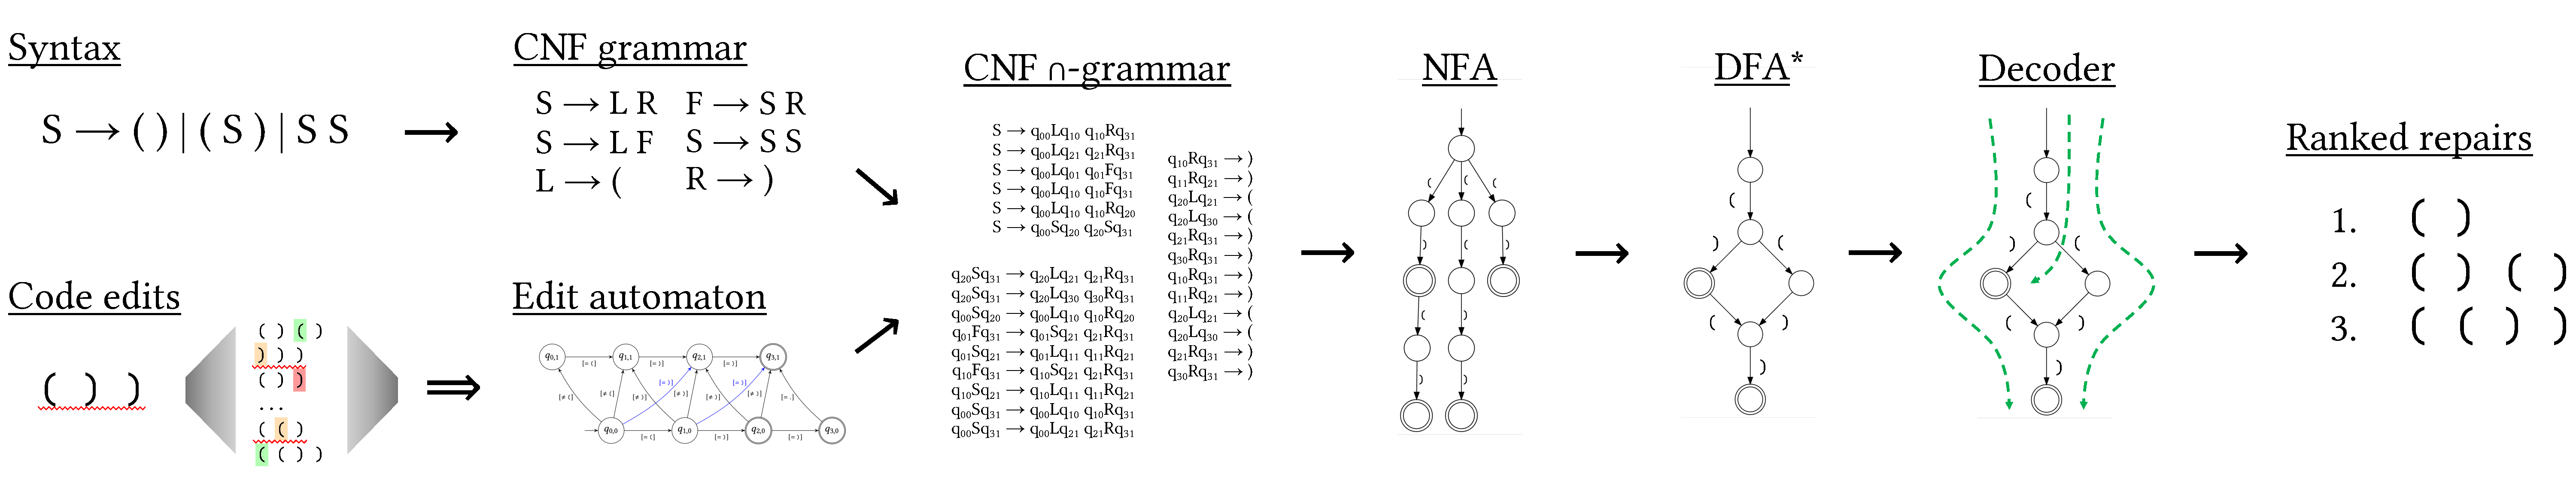
\includegraphics[width=\textwidth]{flow}\vspace{-1pt}
    \caption{Simplified dataflow. Given a grammar and broken code fragment, we create an automaton generating the language of small edits, then construct a grammar representing the intersection of the two languages. This grammar can be converted to a finite automaton, determinized, then decoded to produce a list of repairs.}\label{fig:arch_simp}
  \end{figure}

  \noindent This process is depicted in Fig.~\ref{fig:arch_simp}. We will now discuss the intersection step in slightly more detail.

  \clearpage

  By way of illustration, suppose we have a string $\texttt{( ) )}$, and wish to find nearby repairs. To represent the language of small edits, there is an automaton, called the Levenshtein automaton, recognizing every single string that can be formed by inserting, substituting or deleting a parenthesis. We use a variant that removes some unnecessary arcs but does not affect the generated language.

\begin{figure}[h!]
  \resizebox{0.45\textwidth}{!}{
  \begin{tikzpicture}[
%->, % makes the edges directed
    >=stealth',
    node distance=2.5cm, % specifies the minimum distance between two nodes. Change if necessary.
%  every state/.style={thick, fill=gray!10}, % sets the properties for each ’state’ node
    initial text=$ $, % sets the text that appears on the start arrow
  ]
    \node[state, initial]                (00) {$q_{0,0}$};
    \node[state, right of=00]            (10) {$q_{1,0}$};
    \node[accepting, state, right of=10] (20) {$q_{2,0}$};
    \node[accepting, state, right of=20] (30) {$q_{3,0}$};

    \node[state, above of=00, shift={(-2cm,0cm)}] (01) {$q_{0,1}$};
    \node[state, right of=01]                     (11) {$q_{1,1}$};
    \node[state, right of=11]                     (21) {$q_{2,1}$};
    \node[accepting, state, right of=21]          (31) {$q_{3,1}$};

    \draw [->] (00) edge[below] node{$\texttt{(}$} (10);
    \draw [->] (10) edge[below] node{$\texttt{)}$} (20);
    \draw [->] (20) edge[below] node{$\texttt{)}$} (30);

    \draw [->] (01) edge[below] node{$\texttt{(}$}                       (11);
    \draw [->] (11) edge[below] node[shift={(-0.2cm,0cm)}]{$\texttt{)}$} (21);
    \draw [->] (21) edge[below] node[shift={(-0.2cm,0cm)}]{$\texttt{)}$} (31);

    \draw [->] (00) edge[bend left=10] node[shift={(-0.15cm,0cm)}]{\tiny{$\texttt{(}$}} (11);
    \draw [->] (10) edge[bend left=10] node[shift={(-0.15cm,0cm)}]{\tiny{$\texttt{(}$}} (21);
    \draw [->] (20) edge[bend left=10] node[shift={(-0.15cm,0cm)}]{\tiny{$\texttt{(}$}} (31);

    \draw [->] (00) edge[bend left=10, left] node[shift={(-0.1cm,0cm)}]{\tiny{$\texttt{(}$}} (01);
    \draw [->] (10) edge[bend left=10, left] node[shift={(-0.1cm,0cm)}]{\tiny{$\texttt{(}$}} (11);
    \draw [->] (20) edge[bend left=10, left] node[shift={(-0.1cm,0cm)}]{\tiny{$\texttt{(}$}} (21);

    \draw [->] (00) edge[bend right=10, right] node{\tiny{$\texttt{)}$}} (11);
    \draw [->] (10) edge[bend right=10, right] node{\tiny{$\texttt{)}$}} (21);
    \draw [->] (20) edge[bend right=10, right] node{\tiny{$\texttt{)}$}} (31);

    \draw [->] (00) edge[bend right=10, right] node{\tiny{$\texttt{)}$}} (01);
    \draw [->] (10) edge[bend right=10, right] node{\tiny{$\texttt{)}$}} (11);
    \draw [->] (20) edge[bend right=10, right] node{\tiny{$\texttt{)}$}} (21);

    \draw [->] (30) edge[bend left=10, left] node[shift={(-0.1cm,0cm)}]{\tiny{$\texttt{(}$}} (31);
    \draw [->] (30) edge[bend right=10, right] node{\tiny{$\texttt{)}$}} (31);

    \draw [->, blue] (00) edge[bend right=11,below] node[shift={(0.4cm,0.9cm)}]{$\texttt{)}$}    (21);
    \draw [->, blue] (10) edge[bend right=11,below] node[shift={(0.4cm,0.9cm)}]{$\texttt{)}$}    (31);
    \node[align=center, yshift=2em, xshift=-1cm] (title) at (current bounding box.north) {Original Levenshtein automaton};
  \end{tikzpicture}
  }
  \resizebox{0.515\textwidth}{!}{
    \begin{tikzpicture}[
%->, % makes the edges directed
      >=stealth',
      node distance=2.5cm, % specifies the minimum distance between two nodes. Change if necessary.
%  every state/.style={thick, fill=gray!10}, % sets the properties for each ’state’ node
      initial text=$ $, % sets the text that appears on the start arrow
    ]
      \draw[orange,->] (-4cm,1.2cm) -- (-3cm,1.2cm);

      \node[state, initial]                (00) {$q_{0,0}$};
      \node[state, right of=00]            (10) {$q_{1,0}$};
      \node[accepting, state, right of=10] (20) {$q_{2,0}$};
      \node[accepting, state, right of=20] (30) {$q_{3,0}$};

      \node[state, above of=00, shift={(-2cm,0cm)}] (01) {$q_{0,1}$};
      \node[state, right of=01]                     (11) {$q_{1,1}$};
      \node[state, right of=11]                     (21) {$q_{2,1}$};
      \node[accepting, state, right of=21]          (31) {$q_{3,1}$};

      \draw [->] (00) edge[below] node{\tiny{$[= \texttt{(}]$}} (10);
      \draw [->] (10) edge[below] node{\tiny{$[= \texttt{)}]$}} (20);
      \draw [->] (20) edge[below] node{\tiny{$[= \texttt{)}]$}} (30);

      \draw [->] (01) edge[below] node{\tiny{$[= \texttt{(}]$}}                       (11);
      \draw [->] (11) edge[below] node[shift={(-0.2cm,0cm)}]{\tiny{$[= \texttt{)}]$}} (21);
      \draw [->] (21) edge[below] node[shift={(-0.2cm,0cm)}]{\tiny{$[= \texttt{)}]$}} (31);

      \draw [->] (00) edge[left] node{\tiny{$[\neq \texttt{(}]$}} (11);
      \draw [->] (10) edge[left] node{\tiny{$[\neq \texttt{)}]$}} (21);
      \draw [->] (20) edge[left] node{\tiny{$[\neq \texttt{)}]$}} (31);

      \draw [->] (00) edge[bend left=10, left] node{\tiny{$[\neq \texttt{(}]$}} (01);
      \draw [->] (10) edge[bend left=10, left] node{\tiny{$[\neq \texttt{)}]$}} (11);
      \draw [->] (20) edge[bend left=10, left] node{\tiny{$[\neq \texttt{)}]$}} (21);
      \draw [->] (30) edge[bend left=10, left] node{\tiny{$[=.]$}} (31);


      \draw [->, blue] (00) edge[bend right=11,below] node[shift={(0.2cm,0.8cm)}]{\tiny{$[= \texttt{)}]$}}    (21);
      \draw [->, blue] (10) edge[bend right=11,below] node[shift={(0.2cm,0.8cm)}]{\tiny{$[= \texttt{)}]$}}    (31);
      \node[align=center, yshift=2em, xshift=-0.4cm] (title) at (current bounding box.north) {Nominal Levenshtein automaton (ours)};
    \end{tikzpicture}
  }
  \caption{Automaton recognizing every 1-edit patch. We nominalize the original automaton, ensuring upward arcs denote a mutation, and use a symbolic predicate, which deduplicates parallel arcs in large alphabets.}\label{fig:lev_automaton}\vspace{-5pt}
\end{figure}

Let us consider a very simple grammar: $G = \{S \rightarrow ( ) \mid ( S ) \mid S S\}$. For convenience, $G$ can be reduced into an equivalent normal form, $G'$, by refactoring the right-hand side of each production to be in either binary or unary form: $G'= \{S \rightarrow L R, S \rightarrow L F, S \rightarrow S S, F \rightarrow S R, L \rightarrow (, R \rightarrow )\}$. Now, we proceed to stitch together the automaton and grammar into new grammar, $G_\cap$, that will recognize every string in the intersection of their respective languages, and no other string.

This stitching process is known in the literature as the Bar-Hillel (BH) construction, and applies to any context-free grammar and nondeterministic finite automaton. It has three rules: first, for every initial state in the automaton (here there is just one, $q_{00}$) and every final state, ($q_{20}, q_{30}, q_{31}$), there will be a production $S\rightarrow q_{00}Sq_{xy}$. We call this rule $\sqrt{\phantom{S}}$, and leave it unchanged.

Next, the BH construction states: for every production $A\rightarrow a$ and arc $q \overset{a}{\rightarrow} q'$ in the automaton, there will be a production, $qAq'\rightarrow a$ in the intersection grammar. Here is where our variation, the Levenshtein Bar-Hillel (LBH) construction, now diverges: we only consider unit productions matching the nominal predicate depicted in Fig.~\ref{fig:lev_automaton}, and will call this modified rule $\hat\uparrow$.

So far, the intersection grammar now contains the following productions:\vspace{-5pt}

\begin{table}[H]
  \begin{tabular}{cc|ccccccccccccc}
    $\sqrt{\phantom{S}}$ & & & & & & $\hat\uparrow$ & \\\hline
    $S \rightarrow q_{00}Sq_{20}$ & & & $q_{00}Rq_{01} \rightarrow \texttt{)}$ & & $q_{10}Lq_{11} \rightarrow \texttt{(}$ & & $q_{20}Rq_{21} \rightarrow \texttt{)}$ & & $q_{01}Lq_{11} \rightarrow \texttt{(}$ \\
    $S \rightarrow q_{00}Sq_{30}$ & & & $q_{00}Rq_{11} \rightarrow \texttt{)}$ & & $q_{10}Lq_{21} \rightarrow \texttt{(}$ & & $q_{20}Rq_{31} \rightarrow \texttt{)}$ & & $q_{11}Rq_{21} \rightarrow \texttt{)}$ \\
    $S \rightarrow q_{00}Sq_{31}$ & & & $q_{00}Lq_{10} \rightarrow \texttt{(}$ & & $q_{10}Rq_{20} \rightarrow \texttt{)}$ & & $q_{20}Lq_{30} \rightarrow \texttt{(}$ & & $q_{21}Rq_{31} \rightarrow \texttt{)}$ \\
                                  & & & $q_{30}Lq_{31} \rightarrow \texttt{(}$ & & $q_{10}Rq_{31} \rightarrow \texttt{)}$ & & $q_{30}Rq_{31} \rightarrow \texttt{)}$ & & $q_{00}Rq_{21} \rightarrow \texttt{)}$
  \end{tabular}
\end{table}\vspace{-8pt}

The final and most expensive rule of the BH construction, $\Join$, stipulates: for every $w \rightarrow xz$ in $G'$ and every state triplet $\langle p, q, r\rangle$, we will have $pwr \rightarrow (pxq)(qzr)$ in $G_\cap$. This rule creates a synthetic production recognizing every combination of NFA states consistent with every nonterminal in every production. Fortunately, most of these combinations are simply impossible. For example, we note that $q_{31}Sq_{00}$ is an impossible nonterminal, as there is no path from $q_{31}$ to $q_{00}$ in the Levenshtein automaton (Fig.~\ref{fig:lev_automaton}). Likewise, the nonterminal $q_{i, j}Fq_{i+1, j}$ is clearly impossible, as the nonterminal $F$ requires at least three tokens, and the only path from $q_{i, j}$ to $q_{i+1, j}$ has length one. Criteria such as these are essential for filtering out synthetic nonterminals generated by the original BH $\Join$ rule.

%One useful heuristic is to precompute a table for each nonterminal in the grammar $G'$ of lower and upper bounds on the Parikh image, $[l, u]$, counting the number of terminals that any string of exactly length $n$, generated by a nonterminal $v$, must contain ($l$), and may contain ($u$). Once computed, this table can be reused for any repair. Leaving aside the precise details of its construction, we present the Parikh map for the grammar $G'$ below, for $n\in [1,4]$:
%
%\begin{table}[H]
%  \begin{tabular}{|*{17}{c|}} \hline
%    & \multicolumn{4}{c|}{n = 1} & \multicolumn{4}{c|}{n = 2} & \multicolumn{4}{c|}{n = 3} & \multicolumn{4}{c|}{n = 4} \\\cline{3-17}\hline
%               & S        & L        & R        & I        &   S        & L        & R        & I        &    S        & L        & R        & I        &    S        & L        & R        & I        \\\hline
%    \texttt{(} & $\varnothing$ & $[1, 1]$ & $\varnothing$ & $\varnothing$ &   $[1, 1]$ & $\varnothing$ & $\varnothing$ & $\varnothing$ &    $\varnothing$ & $\varnothing$ & $\varnothing$ & $[1, 1]$ &    $[2, 2]$ & $\varnothing$ & $\varnothing$ & $\varnothing$ \\\hline
%    \texttt{)} & $\varnothing$ & $\varnothing$ & $[1, 1]$ & $\varnothing$ &   $[1, 1]$ & $\varnothing$ & $\varnothing$ & $\varnothing$ &    $\varnothing$ & $\varnothing$ & $\varnothing$ & $[2, 2]$ &    $[2, 2]$ & $\varnothing$ & $\varnothing$ & $\varnothing$ \\\hline
%  \end{tabular}
%\end{table}
%
%Now, when considering the triple $q_{10}Iq_{21}$, we know that states $q_{10}, q_{21}$ have paths ranging from length 1 to 2, and the nonterminal $I$ can be no shorter than 3 terminals. Therefore $I$ is incompatible with $q_{10}, q_{21}$ by length, as is any synthetic production containing it.

In Sec.~\ref{sec:lev_bh}, we will consider a refinement to the $\Join$ rule which eliminates many impossible productions from BH intersection grammars by a sound overapproximation to the Parikh image. Aggressively pruning synthetic productions from $G_\cap$ by (1) nominalizing the Levenshtein automaton and (2) refining the $\Join$ rule, are key insights to unlocking the full potential of the Bar-Hillel construction and scaling up this technique to handle real-world program repair scenarios.

  \clearpage\section{Problem statement}\label{sec:problem}

  Source code in a programming language can be treated as a string over a finite alphabet, $\Sigma$. We use a lexical alphabet for convenience. The language has a syntax, $\ell \subset \Sigma^*$, containing every acceptable program. A syntax error is an unacceptable string, $\err\sigma \notin \ell$. We can model syntax repair as a language intersection between a context-free language (CFL) and a regular language. Henceforth, $\err\sigma$ will always and only be used to denote a syntactically invalid string whose target language is known.

  \begin{definition}[Bounded Levenshtein-CFL reachability]\label{def:bcflr}
    Given a CFL, $\ell$, and an invalid string, $\err{\sigma}: \bar\ell$, find every valid string reachable within $d$ edits of $\err{\sigma}$, i.e., letting $\Delta$ be the Levenshtein metric and $L(\err\sigma, d) = \{\sigma' \mid \Delta(\err{\sigma}, \sigma') \leq d\}$ be the Levenshtein $d$-ball, we seek to find $\ell_\cap = L(\err\sigma, d) \cap \ell$.
  \end{definition}

%  To solve this problem, it is convenient to first consider intersections with a finite-length string with holes, then turn our attention back to BCFLR.
%

  As the admissible set $\ell_\cap$ is typically under-constrained, we want a procedure which surfaces natural and valid repairs over unnatural but valid repairs:

  \begin{definition}[Ranked repair]\label{def:ranked-repair}
    Given a finite language $\ell_\cap = L(\err\sigma, d) \cap \ell$ and a probabilistic language model $\text{P}_\theta: \Sigma^* \rightarrow [0, 1] \subset \mathbb{R}$, the ranked repair problem is to find the top-$k$ maximum likelihood repairs under the language model. That is,
    \begin{equation}
      R(A, P_\theta) = \argmax_{\bm{\sigma} \subseteq \ell_\cap, |\bm{\sigma}| \leq k} \sum_{\sigma \in \bm{\sigma}}\text{P}_\theta(\sigma)
    \end{equation}
    % On average, across all $G, \sigma$ $\hat{R}$ should approximate $R$.
%    We want a procedure $\hat{R}$, minimizing $\mathbb{E}_{G, \sigma}\big[D_{\text{KL}}(\hat{R} \parallel R)\big]$ and wallclock runtime.
  \end{definition}

  A popular approach to ranked repair involves learning a distribution over strings, however this is highly sample-inefficient and generalizes poorly to new languages. Approximating a distribution over $\Sigma^*$ forces the model to jointly learn syntax and stylometry. Furthermore, even with an extremely efficient approximate sampler for $\sigma \sim \ell_\cap$, due to the size of $\ell$ and $L(\err\sigma, d)$, it would be intractable to sample either $\ell$ or $L(\err\sigma, d)$, reject duplicates, then reject invalid ($\sigma \notin \ell$) or unreachable $\big(\sigma \notin L(\err\sigma, d)\big)$ edits, and completely out of the question to sample $\sigma \sim \Sigma^*$ as do many neural language models.

  As we will demonstrate, the ranked repair problem can be factorized into a bilevel objective: first maximal retrieval, then ranking. Instead of working with strings, we will explicitly construct a grammar which soundly and completely generates the set $\ell \cap L(\err\sigma, d)$, then retrieve repairs from its language. By ensuring retrieval is sufficiently precise and exhaustive, maximizing likelihood over the retrieved set can be achieved with a much simpler, syntax-oblivious language model.

  Assuming we have a grammar that recognizes the Levenshtein-CFL intersection, the question then becomes how to maximize the number of unique valid sentences in a given number of samples. Top-down incremental sampling with replacement eventually converges to the language, but does so superlinearly~\cite{flajolet1992birthday}. Due to practical considerations including latency, we require the sampler to converge linearly, ensuring with much higher probability that natural repairs are retrieved in a timely manner. This motivates the need for a specialized generating function. More precisely,

  \begin{definition}[Linear convergence]\label{def:linear-convergence}
    Given a finite CFL, $\ell$, we want a randomized generating function, $\bm{\varphi}: \mathbb{N}_{\leq|\ell|} \rightarrow 2^\ell$, whose rate of convergence is linear in expectation, i.e., $\mathbb{E}_{i \in [1, n]}|\bm{\varphi}(i)| \propto n$.
  \end{definition}

  \noindent This will ensure that if $|\ell_\cap|$ is sufficiently small and enough samples are drawn, $\bm\varphi$ is sure to include a representative subset, and additionally, will terminate after exhausting all valid repairs.

  To satisfy Def.~\ref{def:linear-convergence}, we can construct a bijection from syntax trees to integers (\S~\ref{sec:ptree}), sample integers uniformly without replacement, then decode them as trees. This will produce a set of unique trees, and each tree, assuming grammatical unambiguity, will correspond to a unique sentence in the language.  Finally, sentences can be scored and ranked by likelihood under a language model.

  Otherwise, if the grammar, $G_\ell$, is ambiguous, it can be translated into a DFA, then decoded (\S~\ref{sec:decoding}) using an autoregressive language model or any suitably fast scoring function of the implementer's choice. In our case, we use a low-order Markov model for its inference speed, data efficiency, and simplicity. So long as the decoder samples $\ell$ without replacement, it will satisfy Def.~\ref{def:linear-convergence}.

%  Finally, once we have a set of small and valid repairs, the problem of ranked repair reduces to sorting retrieved samples by likelihood, which can be approximated using an autoregressive language model or any suitable scoring function of the implementer's choice.

  \clearpage\section{Method}

  The method we describe in this paper takes as input the invalid code fragment, and returns a set of plausible repairs. We assume to know the target syntax and a small dataset of valid programs to estimate the likelihood of candidate repairs. At a high level, our method can be decomposed into two main steps: (1) language intersection, (2) repair decoding.

First, we generate a synthetic grammar representing the intersection between the syntax and the Levenshtein ball around the source code, then during the decoding process, retrieve as many repairs as possible from the intersection grammar via enumeration or trajectory sampling, then rerank all unique repairs by naturalness. This can be depicted in more detail as a flowchart (Fig.~\ref{fig:flowchart}).

  \begin{wrapfigure}{r}{0.4\textwidth}
%\begin{figure}[h!]
    \vspace{-0.4cm}
    \begin{center}
      \resizebox{0.4\textwidth}{!}{
        \begin{tikzpicture}[node distance=2cm]
          \node (start) [startstop, draw=none];
          \node (pro1) [process, below of=start, yshift=-0.3cm] {$G_\cap \gets G\cap L(\err\sigma, d)$};
          \node [above=0.07cm of pro1] {(\S~\ref{sec:lev_bh})};
          \node (pcfg) [io2, left of=pro1, xshift=-3cm] {CFG};
          \node [above=0.07cm of pcfg, xshift=1cm] {(\S~\ref{sec:prelim})};
          \node (lnfa) [io, right of=pro1, xshift=3cm] {L-NFA};
          \node [above=0.07cm of lnfa, xshift=1cm] {(\S~\ref{sec:lev_nfa})};

          \node (code) [io, right of=start,xshift=3cm] {Code};
          \node (synt) [io2, left of=start,xshift=-3cm] {Syntax};

          \node (dec1) [decision, below of=pro1, yshift=-0.5cm] {$[G_{\cap} = \varnothing]$};

          \node (t2) [process, left of=dec1, xshift=-3cm] {Construct $\mathbb{T}_2$ from $G_\cap'$};

          \node (pro2b) [process, right of=dec1, xshift=3cm] {Increase radius, $d$};

          \node [below=0.7cm of pro2b, xshift=0.05cm] {\Large\textbf{Language intersection}};
          \draw[thick,dotted, rounded corners] ($(pcfg.north west)+(-1.9,0.8)$) rectangle ($(pro2b.south east)+(0.3,-1.5)$);

          \node (const) [process, below of=dec1, yshift=-1.8cm, xshift=-1.5cm] {Enumerate trees from $\mathbb{T}_2$};
          \node [above=0.07cm of const, xshift=1.5cm] {(\S~\ref{sec:tree_sampling})};

%          \node (dec2) [decision, below of=const, yshift=-0.5cm] {$|\mathcal{L}(G_\cap)|$};
%
%          \node (samp1) [process, left of=dec2, xshift=-3cm] {Enumerate $\sigma' \in \mathcal{L}(G_\cap)$};
%          \node [above=0.07cm of samp1] {(\S~\ref{sec:ptree})};
%          \node (samp2) [process, right of=dec2, xshift=3cm] {Sample $\sigma' \sim P(G_\cap)$};
%          \node [above=0.07cm of samp2] {(\S~\ref{sec:ptree})};

%          \draw[thick,dotted, rounded corners] ($(const.north west)+(-5.3,0.7)$) rectangle ($(samp2.south east)+(0.3,-0.6)$);

          \node (rrpc) [process, below of=const, yshift=-0.5cm] {Rerank by PCFG score};
          \node [above=0.07cm of rrpc, xshift=1.7cm] {(Algorithm 1, \S~\ref{sec:ranking})};
          \node (rank) [process, below of=rrpc, yshift=-0.5cm] {Convert to DFA and walk};
          \node [above=0.1cm of rank, xshift=1.7cm] {(Algorithm 3, \S~\ref{sec:decoding})};
%          \node (vlmc) [io2, right of=rank, xshift=3cm] {Markov chain};
          \node [below=0.3cm of rank, xshift=-4cm] {\Large\textbf{Repair decoding}};
          \draw [thick,dotted, rounded corners] ($(rank.north west)+(-3.8,5.8)$) rectangle ($(rank.south east)+(6.8,-1.1)$);

          \node (rrng) [process, right of=const, xshift=4.5cm] {Rerank by n-gram score};
          \node [above=0.1cm of rrng, xshift=0.7cm] {(Algorithm 2, \S~\ref{sec:ranking})};
          \node (results) [io, right of=rank, xshift=4.5cm] {Repairs};
%  \node (out1) [io, below of=pro2a] {Output};
          \node (stop) [startstop, right of=rank, xshift=3cm];
          \node (stop1) [startstop, right of=rrpc, xshift=3cm];
          \node (stop2) [startstop, right of=const, xshift=3cm];

%  \draw [arrow] (dec0) -- node[anchor=east] {no} (pro1);

%          \draw [->,thick] (-5, 1.3) -- (synt);
%          \draw [->,thick] (5, 1.3) -- (code);

%          \draw [arrow] (start) -- (code);
%          \draw [arrow] (start) -- (synt);
          \draw [arrow] (code) -- (lnfa);
          \draw [arrow] (const) -- (rrng);
          \draw [arrow] (rrng) -- (results);
          \draw [arrow] (synt) -- (pcfg);
          \draw [arrow] (lnfa) -- (pro1);
          \draw [arrow] (pcfg) -- (pro1);

%          \draw [arrow] (grwa) -- (results);
%          \draw [line width=0.8pt] (stop.west) -- (stop1.west);
%          \draw [line width=0.8pt] (stop2.west) -- (stop1.west);

%  \draw [arrow] (in1) -- (pro1);
          \draw [arrow] (pro1) -- (dec1);
          \draw [arrow] (dec1) -- node[anchor=south] {yes} (pro2b);
          \draw [arrow] (dec1) -- node[anchor=south] {no} (t2);
          \draw [arrow] (const) -- (rrpc);
          \draw [arrow] (pro2b) -- (lnfa);
%          \draw [arrow] (dec2) -- node[anchor=south] {small} (samp1);
%          \draw [arrow] (dec2) -- node[anchor=south] {large} (samp2);

          \draw [arrow] (t2) |- ([shift={(-1.3cm,0)}]const.west)--(const.west);
%          \draw [arrow] (t2) |- ([shift={(-1.3cm,0)}]grwa.west)--(grwa.west);
          \draw [arrow] (t2) |- ([shift={(-1.3cm,0)}]rank.west)--(rank.west);
%          \draw [arrow] (vlmc) -- (rank);
          \draw [arrow] (rrpc) |- ([shift={(4.37cm,0)}]rrpc.east)--(results.north);
%          \draw [arrow] (samp2) |- ([shift={(0,1.3cm)}]rank.north)--(rank.north);
%  \draw [arrow] (pro2a) -- (out1);
          \draw [arrow] (rank) -- (results);
%          \draw [line width=0.8pt] (grwa) -- (stop1);
%          \draw [line width=0.8pt] (const) -- (stop2);
%          \draw [arrow] (dec2) -- node[anchor=east] {1} (stop);

        \end{tikzpicture}
      }
    \end{center}
%    \vspace{-0.7cm}
    \caption{Dataflow of our proposed method.}\label{fig:flowchart}
    \vspace{-0.5cm}
  \end{wrapfigure}

  More specifically, since the syntax of most programming languages is context-free, we construct a context-free grammar (CFG), $G_\cap$, representing the intersection between the programming language syntax ($G$) and an automaton recognizing the Levenshtein edit ball of a given radius, $L(\err\sigma, d)$. As the CFL family is closed under intersection with regular languages, the intersection language $\mathcal{L}(G_\cap)$ should contain every repair within a given Levenshtein distance and no invalid repairs. Either the grammar will be empty, in which case there are no repairs within the given radius, or it will be nonempty, in which case we can directly proceed to decode the repairs.

%  \begin{enumerate}
%    \item $G_\cap$ is empty, in which case there is no repair within the given radius. In this case, we simply increase the radius and try again.
%    \item $\mathcal{L}(G_\cap)$ is small, in which case we enumerate all possible repairs. Complete enumeration is tractable for the majority of all syntax repairs.
%    \item $\mathcal{L}(G_\cap)$ is too large to completely enumerate, so we sample instead from $G_\cap$, top-down. Sampling is necessary for a minority of remaining cases.
%  \end{enumerate}

  We present three basic methods for repair decoding: enumerate parse trees from the CFG, $G_\cap$, and rerank each tree by either (1) PCFG score, or (2) Markov chain likelihood, or (3) translate $G_\cap$ to an equivalent DFA, $\mathcal{A}_\cap$, minimize it using Brzozowski's algorithm to produce $\mathcal{A}_\cap^*$, then sample trajectories without replacement through the DFA according to a Markov chain until a fixed timeout is reached. We use (3) by default but will present a comparison of (1-3) in \S~\ref{sec:rq3}.

  In all cases, if the language is sufficiently small, this will generate every possible repair and halt early. Otherwise, if the language is too large to exhaustively search, it will draw a representative subset containing the most likely repairs with high probability, then halt. The decoders (1-3) essentially differ in the order they retrieve repairs, and the likelihood model they use to rank them.

  We will first describe how to generate the intersection grammar (\S~\ref{sec:lev_nfa},~\ref{sec:lev_bh}), then, define a data structure compactly representing its language, allowing us to efficiently decode all repairs contained within (\S~\ref{sec:ptree}). Finally, we will show how to enumerate repairs from the CFG (\S~\ref{sec:tree_sampling}), or sample them from an equivalent DFA (\S~\ref{sec:decoding}). As we build up our intuition for each component, we will periodically revisit the criteria from \S~\ref{sec:problem}, to ensure we remain on the right track.

  \subsection{Preliminaries}\label{sec:prelim}

  Recall that a CFG, $\mathcal{G} = \langle \Sigma, V, P, S\rangle$, is a quadruple consisting of terminals $(\Sigma)$, nonterminals $(V)$, productions $(P\colon V \rightarrow (V \mid \Sigma)^*)$, and a start symbol, $(S)$. Every CFG is reducible to so-called \textit{Chomsky Normal Form}~\cite{chomsky1959certain}, $P'\colon V \rightarrow (V^2 \mid \Sigma)$, where every production is either (1) a binary production $w \rightarrow xz$, or (2) a unit production $w \rightarrow t$, where $w, x, z: V$ and $t: \Sigma$. For example:\vspace{-3pt}

  \begin{table}[H]
    \begin{tabular}{llll}
      $G = \big\{\;S \rightarrow S\:S \mid (\:S\:) \mid (\:)\;\big\} \Longrightarrow G' = \big\{\;S\rightarrow Q\:R \mid S\:S \mid L\:R,$ & $R \rightarrow\:),$ & $L \rightarrow (,$ & $Q\rightarrow L\:S\;\big\}$
    \end{tabular}
  \end{table}\vspace{-8pt}

  Likewise, a finite state automaton (FSA) is a quintuple $\mathcal{A} = \langle Q, \Sigma, \delta, I, F\rangle$, where $Q$ is a finite set of states, $\Sigma$ is a finite alphabet, $\delta \subseteq Q \times \Sigma \times Q$ is the transition function, and $I, F \subseteq Q$ are the set of initial and final states, respectively. We will adhere to this notation in the following sections.

  \clearpage\subsection{Modeling lexical edits with the nominal Levenshtein automaton}\label{sec:lev_nfa}

  \begin{wrapfigure}{r}{0.5\textwidth}
    \vspace{-0.3cm}
    \begin{center}
        \resizebox{0.8\textwidth}{!}{
  \begin{tikzpicture}[
%->, % makes the edges directed
  >=stealth',
  node distance=2.5cm, % specifies the minimum distance between two nodes. Change if necessary.
%  every state/.style={thick, fill=gray!10}, % sets the properties for each ’state’ node
  initial text=$ $, % sets the text that appears on the start arrow
  ]
  \node[state, initial]                (00) {$q_{0,0}$};
  \node[state, right of=00]            (10) {$q_{1,0}$};
  \node[accepting, state, right of=10] (20) {$q_{2,0}$};
  \node[accepting, state, right of=20] (30) {$q_{3,0}$};
  \node[accepting, state, right of=30] (40) {$q_{4,0}$};
  \node[accepting, state, right of=40] (50) {$q_{5,0}$};

  \node[state, above of=00, shift={(-2cm,0cm)}] (01) {$q_{0,1}$};
  \node[state, right of=01]                          (11) {$q_{1,1}$};
  \node[state, right of=11]                          (21) {$q_{2,1}$};
  \node[accepting, state, right of=21]               (31) {$q_{3,1}$};
  \node[accepting, state, right of=31]               (41) {$q_{4,1}$};
  \node[accepting, state, right of=41]               (51) {$q_{5,1}$};

\node[state, above of=01, shift={(-2cm,0cm)}] (0j) {$q_{0,2}$};
\node[state, right of=0j]                          (1j) {$q_{1,2}$};
\node[state, right of=1j]                          (2j) {$q_{2,2}$};
\node[state, right of=2j]                          (3j) {$q_{3,2}$};
\node[accepting, state, right of=3j]               (4j) {$q_{4,2}$};
\node[accepting, state, right of=4j]               (5j) {$q_{5,2}$};

\node[state, above of=0j, shift={(-2cm,0cm)}] (0k) {$q_{0,3}$};
\node[state, right of=0k]                         (1k) {$q_{1,3}$};
\node[state, right of=1k]                         (2k) {$q_{2,3}$};
\node[state, right of=2k]                         (3k) {$q_{3,3}$};
\node[state, right of=3k]                         (4k) {$q_{4,3}$};
\node[accepting, state, right of=4k]              (5k) {$q_{5,3}$};

\draw [->] (00) edge[below] node{$\sigma_1$} (10);
\draw [->] (10) edge[below] node{$\sigma_2$} (20);
\draw [->] (20) edge[below] node{$\sigma_3$} (30);
\draw [->] (30) edge[below] node{$\sigma_4$} (40);
\draw [->] (40) edge[below] node{$\sigma_5$} (50);

\draw [->] (01) edge[below] node{$\sigma_1$} (11);
\draw [->] (11) edge[below] node[shift={(-0.2cm,0cm)}]{$\sigma_2$} (21);
\draw [->] (21) edge[below] node[shift={(-0.2cm,0cm)}]{$\sigma_3$} (31);
\draw [->] (31) edge[below] node[shift={(-0.2cm,0cm)}]{$\sigma_4$} (41);
\draw [->] (41) edge[below] node{$\sigma_5$} (51);

\draw [->] (0j) edge[below] node{$\sigma_1$} (1j);
\draw [->] (1j) edge[below] node{$\sigma_2$} (2j);
\draw [->] (2j) edge[below] node{$\sigma_3$} (3j);
\draw [->] (3j) edge[below] node{$\sigma_4$} (4j);
\draw [->] (4j) edge[below] node{$\sigma_5$} (5j);

\draw [->] (0k) edge[below] node{$\sigma_1$} (1k);
\draw [->] (1k) edge[below] node{$\sigma_2$} (2k);
\draw [->] (2k) edge[below] node{$\sigma_3$} (3k);
\draw [->] (3k) edge[below] node{$\sigma_4$} (4k);
\draw [->] (4k) edge[below] node{$\sigma_5$} (5k);

\draw [->] (00) edge[left] node{$\phantom{\cdot}$} (11);
\draw [->] (10) edge[left] node{$\phantom{\cdot}$} (21);
\draw [->] (20) edge[left] node{$\phantom{\cdot}$} (31);
\draw [->] (30) edge[left] node{$\phantom{\cdot}$} (41);
\draw [->] (40) edge[left] node{$\phantom{\cdot}$} (51);

% Super-knight arcs
\draw [->, red] (00) edge[bend right=8] node[east, shift={(-0.2cm,-0.7cm)}]{$\color{red}\sigma_3$}         (3j);
\draw [->, red] (10) edge[bend right=8] node[east, shift={(-0.2cm,-0.7cm)}]{$\color{red}\sigma_4$}         (4j);
\draw [->, red] (20) edge[bend right=8] node[east, shift={(-0.2cm,-0.7cm)}]{$\color{red}\sigma_5$}         (5j);

\draw [->, red] (01) edge[bend left=8] node[east, shift={(-0.2cm,-0.7cm)}]{$\color{red}\sigma_3$}         (3k);
\draw [->, red] (11) edge[bend left=8] node[east, shift={(-0.2cm,-0.7cm)}]{$\color{red}\sigma_4$}         (4k);
\draw [->, red] (21) edge[bend left=8] node[east, shift={(-0.2cm,-0.7cm)}]{$\color{red}\sigma_5$}         (5k);

\draw [->, violet] (00) edge node[east, shift={(-0.1cm,-0.8cm)}]{$\color{violet}\sigma_4$}  (4k);
\draw [->, violet] (10) edge node[east, shift={(-0.1cm,-0.8cm)}]{$\color{violet}\sigma_5$}  (5k);

\draw [->] (01) edge[left] node{$\phantom{\cdot}$} (1j);
\draw [->] (11) edge[left] node{$\phantom{\cdot}$} (2j);
\draw [->] (21) edge[left] node{$\phantom{\cdot}$} (3j);
\draw [->] (31) edge[left] node{$\phantom{\cdot}$} (4j);
\draw [->] (41) edge[left] node{$\phantom{\cdot}$} (5j);

\draw [->] (0j) edge[left] node{$\phantom{\cdot}$} (1k);
\draw [->] (1j) edge[left] node{$\phantom{\cdot}$} (2k);
\draw [->] (2j) edge[left] node{$\phantom{\cdot}$} (3k);
\draw [->] (3j) edge[left] node{$\phantom{\cdot}$} (4k);
\draw [->] (4j) edge[left] node{$\phantom{\cdot}$} (5k);

\draw [->] (00) edge[bend left=10, left] node{$\phantom{\cdot}$} (01);
\draw [->] (10) edge[bend left=10, left] node{$\phantom{\cdot}$} (11);
\draw [->] (20) edge[bend left=10, left] node{$\phantom{\cdot}$} (21);
\draw [->] (30) edge[bend left=10, left] node{$\phantom{\cdot}$} (31);
\draw [->] (40) edge[bend left=10, left] node{$\phantom{\cdot}$} (41);
\draw [->] (50) edge[bend left=10, left] node{$\phantom{\cdot}$} (51);

\draw [->] (01) edge[bend left=10, left] node{$\phantom{\cdot}$} (0j);
\draw [->] (11) edge[bend left=10, left] node{$\phantom{\cdot}$} (1j);
\draw [->] (21) edge[bend left=10, left] node{$\phantom{\cdot}$} (2j);
\draw [->] (31) edge[bend left=10, left] node{$\phantom{\cdot}$} (3j);
\draw [->] (41) edge[bend left=10, left] node{$\phantom{\cdot}$} (4j);
\draw [->] (51) edge[bend left=10, left] node{$\phantom{\cdot}$} (5j);

\draw [->] (0j) edge[bend left=10, left] node{$\phantom{\cdot}$} (0k);
\draw [->] (1j) edge[bend left=10, left] node{$\phantom{\cdot}$} (1k);
\draw [->] (2j) edge[bend left=10, left] node{$\phantom{\cdot}$} (2k);
\draw [->] (3j) edge[bend left=10, left] node{$\phantom{\cdot}$} (3k);
\draw [->] (4j) edge[bend left=10, left] node{$\phantom{\cdot}$} (4k);
\draw [->] (5j) edge[bend left=10, left] node{$\phantom{\cdot}$} (5k);

\draw [->, blue] (00) edge[bend right=11,below] node[shift={(0.5cm,0.3cm)}]{$\color{blue}\sigma_2$}    (21);
\draw [->, blue] (10) edge[bend right=11,below] node[shift={(0.5cm,0.3cm)}]{$\color{blue}\sigma_3$}    (31);
\draw [->, blue] (20) edge[bend right=11,below] node[shift={(0.5cm,0.3cm)}]{$\color{blue}\sigma_4$}    (41);
\draw [->, blue] (30) edge[bend right=11,below] node[shift={(0.5cm,0.3cm)}]{$\color{blue}\sigma_5$}    (51);

\draw [->, blue] (01) edge[bend right=3,below] node[shift={(0.3cm,0.2cm)}]{$\color{blue}\sigma_2$}    (2j);
\draw [->, blue] (11) edge[bend right=3,below] node[shift={(0.3cm,0.2cm)}]{$\color{blue}\sigma_3$}    (3j);
\draw [->, blue] (21) edge[bend right=3,below] node[shift={(0.3cm,0.2cm)}]{$\color{blue}\sigma_4$}    (4j);
\draw [->, blue] (31) edge[bend right=3,below] node[shift={(0.3cm,0.2cm)}]{$\color{blue}\sigma_4$}    (5j);

\draw [->, blue] (0j) edge[bend left=8,below] node[shift={(-0.45cm,-0.55cm)}]{$\color{blue}\sigma_2$}    (2k);
\draw [->, blue] (1j) edge[bend left=8,below] node[shift={(-0.45cm,-0.55cm)}]{$\color{blue}\sigma_3$}    (3k);
\draw [->, blue] (2j) edge[bend left=8,below] node[shift={(-0.45cm,-0.55cm)}]{$\color{blue}\sigma_4$}    (4k);
\draw [->, blue] (3j) edge[bend left=8,below] node[shift={(-0.45cm,-0.55cm)}]{$\color{blue}\sigma_5$}    (5k);

%https://tex.stackexchange.com/a/20986/139648
\draw [decorate,decoration={brace,amplitude=10pt,raise=10pt,mirror}] (00.south west) -- (50.south east) node[midway,yshift=-3em]{\textbf{String length}};
\draw [decorate,decoration={brace,amplitude=10pt,raise=20pt}] (00.south west) -- (0k.north west) node[midway,xshift=-1cm,yshift=-1cm,rotate=-54]{\textbf{Edit distance}};
\end{tikzpicture}
}
    \end{center}
    \caption{NFA recognizing Levenshtein $L(\sigma: \Sigma^5, 3)$.}\label{fig:lev_nfa}
    \vspace{-0.5cm}
  \end{wrapfigure}

  Levenshtein edits are recognized by an automaton known as the Levenshtein automaton. As the original construction defined by Schultz and Mihov~\cite{schulz2002fast} contains cycles and $\varepsilon$-transitions, we propose a variant which is $\varepsilon$-free and acyclic. Furthermore, we adopt a nominal form which supports infinite alphabets and considerably simplifies the language intersection to follow. Illustrated in Fig.~\ref{fig:lev_nfa} is an example of a small Levenshtein automaton recognizing $L(\sigma: \Sigma^5, 3)$. Unlabeled arcs accept any terminal from the alphabet, $\Sigma$. Equivalently, this transition system can be viewed as a kind of proof system within an unlabeled lattice. The following construction is equivalent to Schultz and Mihov's original Levenshtein automaton, but is more amenable to our purposes as it does not any contain $\varepsilon$-arcs, and instead uses skip connections to recognize consecutive deletions of varying lengths.

  \begin{prooftree}
    \AxiomC{$s\in\Sigma \phantom{\land} i \in [0, n] \phantom{\land} j \in [1, d_{\max}]$}
    \RightLabel{$\duparrow$}
    \UnaryInfC{$(q_{i, j-1} \overset{s}{\rightarrow} q_{i,j}) \in \delta$}
    \DisplayProof
    \hskip 1.5em
    \AxiomC{$s\in\Sigma \phantom{\land} i \in [1, n] \phantom{\land} j \in [1, d_{\max}]$}
    \RightLabel{$\ddiagarrow$}
    \UnaryInfC{$(q_{i-1, j-1} \overset{s}{\rightarrow} q_{i,j}) \in \delta$}
  \end{prooftree}
  \begin{prooftree}
    \AxiomC{$i \in [1, n] \phantom{\land} j \in [0, d_{\max}]$}
    \RightLabel{$\drightarrow$}
    \UnaryInfC{$(q_{i-1, j} \overset{\sigma_i}{\rightarrow} q_{i,j}) \in \delta$}
    \DisplayProof
    \hskip 1.5em
    \AxiomC{$d \in [1, d_{\max}] \phantom{\land} i \in [d + 1, n] \phantom{\land} j \in [d, d_{\max}]$}
    \RightLabel{$\knightarrow$}
    \UnaryInfC{$(q_{i-d-1, j-d} \overset{\sigma_i}{\rightarrow} q_{i,j}) \in \delta$}
  \end{prooftree}
  \begin{prooftree}
    \AxiomC{$\vphantom{|}$}
    \RightLabel{$\textsc{Init}$}
    \UnaryInfC{$q_{0,0} \in I$}
    \DisplayProof
    \hskip 1.5em
    \AxiomC{$q_{i, j} \in Q$}
    \AxiomC{$|n-i+j| \leq d_{\max}$}
    \RightLabel{$\textsc{Done}$}
    \BinaryInfC{$q_{i, j}\in F$}
  \end{prooftree}

  \newcommand{\substitutionExample}{
    \tikz{
      \foreach \x in {0,8,16,24,32,40}{
        \fill (\x pt,0pt) circle [radius = 1pt];
        \fill (\x pt,8pt) circle [radius = 1pt];
      }
      \phantom{\fill (0pt,-8pt) circle [radius = 1pt];}
      \draw [-to] (0pt,0pt) -- (8pt,0pt);
      \draw [-to] (8pt,0pt) -- (16pt,0pt);
      \draw [-to] (16pt,0pt) -- (24pt,8pt);
      \draw [-to] (24pt,8pt) -- (32pt,8pt);
      \draw [-to] (32pt,8pt) -- (40pt,8pt);
    }
  }

  \newcommand{\insertionExample}{
    \tikz{
      \foreach \x in {0,8,16,24,32,40}{
        \fill (\x pt,0pt) circle [radius = 1pt];
        \fill (\x pt,8pt) circle [radius = 1pt];
      }
      \phantom{\fill (0pt,-8pt) circle [radius = 1pt];}
      \fill[white] (16pt,0pt) circle [radius = 1.2pt];
      \fill[white] (24pt,8pt) circle [radius = 1.2pt];
      \draw [-to] (0pt,0pt) -- (8pt,0pt);
      \draw [-to] (8pt,0pt) -- (24pt,0pt);
      \draw [-to] (24pt,0pt) -- (16pt,8pt);
      \draw [-to] (16pt,8pt) -- (32pt,8pt);
      \draw [-to] (32pt,8pt) -- (40pt,8pt);
    }
  }

  \newcommand{\deletionExample}{
    \tikz{
      \foreach \x in {0,8,16,24,32,40}{
        \fill (\x pt,0pt) circle [radius = 1pt];
        \fill (\x pt,8pt) circle [radius = 1pt];
      }
      \phantom{\fill (0pt,-8pt) circle [radius = 1pt];}
      \draw [-to] (0pt,0pt) -- (8pt,0pt);
      \draw [-to] (8pt,0pt) -- (16pt,0pt);
      \draw [-to] (16pt,0pt) -- (24pt,0pt);
      \draw [-to] (24pt,0pt) -- (40pt,8pt);
    }
  }

  \newcommand{\doubleDeletionExample}{
    \tikz{
      \foreach \x in {0,8,16,24,32,40}{
        \fill (\x pt,0pt) circle [radius = 1pt];
        \fill (\x pt,8pt) circle [radius = 1pt];
        \fill (\x pt,16pt) circle [radius = 1pt];
      }
      \draw [-to] (0pt,0pt) -- (24pt,16pt);
      \draw [-to] (24pt,16pt) -- (32pt,16pt);
      \draw [-to] (32pt,16pt) -- (40pt,16pt);
    }
  }

  \newcommand{\subDelExample}{
    \tikz{
      \foreach \x in {0,8,16,24,32,40}{
        \fill (\x pt,0pt) circle [radius = 1pt];
        \fill (\x pt,8pt) circle [radius = 1pt];
        \fill (\x pt,16pt) circle [radius = 1pt];
      }
      \draw [-to] (0pt,0pt) -- (8pt,0pt);
      \draw [-to] (8pt,0pt) -- (16pt,8pt);
      \draw [-to] (16pt,8pt) -- (32pt,16pt);
      \draw [-to] (32pt,16pt) -- (40pt,16pt);
    }
  }

  \newcommand{\subSubExample}{
    \tikz{
      \foreach \x in {0,8,16,24,32,40}{
        \fill (\x pt,0pt) circle [radius = 1pt];
        \fill (\x pt,8pt) circle [radius = 1pt];
        \fill (\x pt,16pt) circle [radius = 1pt];
      }
      \draw [-to] (0pt,0pt) -- (8pt,0pt);
      \draw [-to] (8pt,0pt) -- (16pt,8pt);
      \draw [-to] (16pt,8pt) -- (24pt,16pt);
      \draw [-to] (24pt,16pt) -- (32pt,16pt);
      \draw [-to] (32pt,16pt) -- (40pt,16pt);
    }
  }

  \newcommand{\insertDeleteExample}{
    \tikz{
      \foreach \x in {0,8,16,24,32,40,48}{
        \fill (\x pt,0pt) circle [radius = 1pt];
        \fill (\x pt,8pt) circle [radius = 1pt];
        \fill (\x pt,16pt) circle [radius = 1pt];
      }
      \fill[white] (16pt,16pt) circle [radius = 1.2pt];
      \fill[white] (8pt,0pt) circle [radius = 1.2pt];
      \fill[white] (16pt,8pt) circle [radius = 1.2pt];
      \draw [-to] (0pt,0pt) -- (16pt,0pt);
      \draw [-to] (16pt,0pt) -- (8pt,8pt);
      \draw [-to] (8pt,8pt) -- (24pt,8pt);
      \draw [-to] (24pt,8pt) -- (40pt,16pt);
      \draw [-to] (40pt,16pt) -- (48pt,16pt);
    }
  }

  Each arc plays a specific role. $\duparrow$ handles insertions, $\ddiagarrow$ handles substitutions and $\knightarrow$ handles deletions of one or more terminals. Let us consider some illustrative cases.

  \begin{table}[h!]
    \begin{tabular}{ccccccc}

      \texttt{f\hspace{3pt}.\hspace{3pt}\hlorange{[}\hspace{3pt}x\hspace{3pt})} &
      \texttt{f\hspace{3pt}.\hspace{3pt}\phantom{(}\hspace{3pt}x\hspace{3pt})} &
      \texttt{f\hspace{3pt}.\hspace{3pt}(\hspace{3pt}\hlred{x}\hspace{3pt})} &
      \texttt{\hlred{.}\hspace{3pt}\hlred{+}\hspace{3pt}(\hspace{3pt}x\hspace{3pt})} &
      \texttt{f\hspace{3pt}\hlorange{.}\hspace{3pt}\hlred{(}\hspace{3pt}x\hspace{3pt};} &
      \texttt{[\hspace{3pt}\hlorange{,}\hspace{3pt}\hlorange{x}\hspace{3pt}y\hspace{3pt}]} &
      \texttt{[\hspace{3pt}\phantom{,}\hspace{3pt},\hspace{3pt}\hlred{x}\hspace{3pt}y\hspace{3pt}]} \\

      \texttt{f\hspace{3pt}.\hspace{3pt}\hlorange{(}\hspace{3pt}x\hspace{3pt})} &
      \texttt{f\hspace{3pt}.\hspace{3pt}\hlgreen{(}\hspace{3pt}x\hspace{3pt})} &
      \texttt{f\hspace{3pt}.\hspace{3pt}(\hspace{3pt}\phantom{x}\hspace{3pt})} &
      \texttt{\phantom{f}\hspace{3pt}\phantom{.}\hspace{3pt}(\hspace{3pt}x\hspace{3pt})} &
      \texttt{f\hspace{3pt}\hlorange{*}\hspace{3pt}\phantom{(}\hspace{3pt}x\hspace{3pt};} &
      \texttt{[\hspace{3pt}\hlorange{x}\hspace{3pt}\hlorange{,}\hspace{3pt}y\hspace{3pt}]} &
      \texttt{[\hspace{3pt}\hlgreen{x}\hspace{3pt},\hspace{3pt}\phantom{x}\hspace{3pt}y\hspace{3pt}]} \\

      \substitutionExample & \insertionExample & \deletionExample & \doubleDeletionExample & \subDelExample & \subSubExample & \insertDeleteExample
    \end{tabular}
  \end{table}

  Note that the same patch can have multiple Levenshtein alignments. $\textsc{Done}$ constructs the final states, which are all states accepting strings $\sigma'$ whose Levenshtein distance $\Delta(\sigma, \sigma') \leq d_\max$.

  To avoid creating a parallel bundle of arcs for each insertion and substitution point, we instead decorate each arc with a nominal predicate, accepting or rejecting $\sigma_i$. To distinguish this nominal variant from the original construction, we highlight the modified rules in orange below.

  \begin{prooftree}
    \AxiomC{$i \in [0, n] \phantom{\land} j \in [1, d_{\max}]$}
    \RightLabel{$\duparrow$}
    \UnaryInfC{$(q_{i, j-1} \overset{{\color{orange}[\neq \sigma_{i+1}]}}{\rightarrow} q_{i,j}) \in \delta$}
    \DisplayProof
    \hskip 1.5em
    \AxiomC{$i \in [1, n] \phantom{\land} j \in [1, d_{\max}]$}
    \RightLabel{$\ddiagarrow$}
    \UnaryInfC{$(q_{i-1, j-1} \overset{{\color{orange}[\neq \sigma_i]}}{\rightarrow} q_{i,j}) \in \delta$}
  \end{prooftree}
  \begin{prooftree}
    \AxiomC{$i \in [1, n] \phantom{\land} j \in [0, d_{\max}]$}
    \RightLabel{$\drightarrow$}
    \UnaryInfC{$(q_{i-1, j} \overset{{\color{orange}[=\sigma_i]}}{\rightarrow} q_{i,j}) \in \delta$}
    \DisplayProof
    \hskip 1.5em
    \AxiomC{$d \in [1, d_{\max}] \phantom{\land} i \in [d + 1, n] \phantom{\land} j \in [d, d_{\max}]$}
    \RightLabel{$\knightarrow$}
    \UnaryInfC{$(q_{i-d-1, j-d} \overset{{\color{orange}[=\sigma_i]}}{\rightarrow} q_{i,j}) \in \delta$}
  \end{prooftree}

  Nominalizing the NFA eliminates the creation of $e=2(|\Sigma| - 1)\cdot|\sigma|\cdot d_\max$ unnecessary arcs over the entire Levenshtein automaton and drastically reduces the size of the construction to follow, but does not affect the underlying semantics. Thus, it is essential to first nominalize the automaton before proceeding to avoid a large blowup in the intermediate grammar.

  \subsection{Recognizing syntactically valid edits via language intersection}\label{sec:lev_bh}

  We now describe the Bar-Hillel construction, which generates a grammar recognizing the intersection between a regular and a context-free language, then specialize it to Levenshtein intersections.

  \begin{lemma}\label{lemma:bar-hillel}
  For any context-free language $\ell$ and finite state automaton $\alpha$, there exists a context-free grammar $G_\cap$ such that $\mathcal{L}(G_\cap) = \ell \cap \mathcal{L}(\alpha)$. See Bar-Hillel~\cite{bar1961formal}.
  \end{lemma}

  \noindent Although Bar-Hillel~\cite{bar1961formal} lacks an explicit construction, Beigel and Gasarch~\cite{beigelproof} construct $G_\cap$ like so:\vspace{-2pt}

  \begin{prooftree}
    \AxiomC{$q \in I \phantom{\land} r \in F\vphantom{\overset{a}{\rightarrow}}$}
    \RightLabel{$\sqrt{\phantom{S}}$}
    \UnaryInfC{$\big(S\rightarrow q S r\big) \in P_\cap$}
    \DisplayProof
    \hskip 1em
    \AxiomC{$(A \rightarrow a) \in P$}
    \AxiomC{$(q\overset{a}{\rightarrow}r) \in \delta$}
    \RightLabel{$\uparrow$}
    \BinaryInfC{$\big(qAr\rightarrow a\big)\in P_\cap$}
    \DisplayProof
    \hskip 1em
%\end{prooftree}
%\begin{prooftree}
    \AxiomC{$(w \rightarrow xz) \in P\vphantom{\overset{a}{\rightarrow}}$}
    \AxiomC{$p,q,r \in Q$}
    \RightLabel{\Join}
    \BinaryInfC{$\big(pwr\rightarrow (pxq)(qzr)\big) \in P_\cap$}
  \end{prooftree}\vspace{2pt}

  This, now standard, Bar-Hillel construction applies to any CFL and REG language intersection, but generates a grammar whose cardinality is approximately $|P_\cap|=|I|\cdot|F| + |P|\cdot|\Sigma|\cdot|\sigma|\cdot2d_{\max} + |P|\cdot|Q|^3$. Applying the BH construction directly to practical languages and code snippets can generate hundreds of trillions of productions for even modestly-sized grammars and Levenshtein automata. Instead, we will describe a kind of reachability analysis that elides many superfluous productions, greatly reducing the number of synthetic productions in the intersection grammar, $G_\cap$.

  Consider $\Join$, the most expensive rule. What $\Join$ tells us is each nonterminal in the intersection grammar $\langle q, v, q'\rangle$ matches a substring simultaneously recognized by (1) a pair of states $q, q'$ in the original NFA and (2) a nonterminal, $v$, in the original CFG. A key observation is that $\Join$ generates the Cartesian product of every such triple, but this is a gross overapproximation for most NFAs and CFGs, as the vast majority of all state pairs and nonterminals recognize no strings in common.

  To identify these superfluous triples, we define an interval domain that soundly overapproximates the Parikh image, encoding the minimum and maximum number of terminals each nonterminal can generate. Since some intervals may be right-unbounded, we write $\mathbb{N}^*=\mathbb{N} \cup \{\infty\}$ to denote the upper bound, and $\Pi = \{[a, b] \in \mathbb{N} \times \mathbb{N}^* \mid a \leq b\}^{|\Sigma|}$ to denote the Parikh image of all terminals.

  \begin{definition}[Parikh mapping of a nonterminal]\label{def:parikh}
    Let $p: \Sigma^*\rightarrow\mathbb{N}^{|\Sigma|}$ be the Parikh operator~\cite{parikh1966context}, which counts the frequency of terminals in a string. We define the Parikh map, $\pi: V \rightarrow \Pi$, as a function returning the smallest interval such that $\forall \sigma: \Sigma^*, \forall v: V$, $v \Rightarrow^* \sigma \vdash p(\sigma) \in \pi(v)$.
  \end{definition}

  In other words, the Parikh mapping computes the greatest lower and least upper bound of the Parikh image over all strings in the language of a nonterminal. The infimum of a nonterminal's Parikh interval tells us how many of each terminal a nonterminal \textit{must} generate, and the supremum tells us how many it \textit{can} generate. Likewise, we define a similar relation over NFA state pairs:

  \begin{definition}[Parikh mapping of NFA states]
    We define $\pi: Q\times Q \rightarrow \Pi$ as returning the smallest interval such that $\forall \sigma: \Sigma^*, \forall q, q': Q$, $q \overset{\sigma}{\Longrightarrow} q' \vdash p(\sigma) \in \pi(q, q')$.
  \end{definition}

  Next, we will define a measure on Parikh intervals representing the minimum total edits required to transform a string in one Parikh interval to a string in another, across all such pairings.

  \begin{definition}[Parikh divergence]
    Given two Parikh intervals $\pi, \pi': \Pi$, we define the divergence between them as $\pi \parallel \pi' = \sum_{n=1}^{|\Sigma|} \min_{(i, i') \in \pi[n]\times \pi'[n]} |i - i'|$.
  \end{definition}

  Now, we know that if the Parikh divergence between two intervals is nonzero, those intervals must be incompatible as no two strings, one from each Parikh interval, can be transformed into the other with fewer than $\pi \parallel \pi'$ edits.

  \begin{definition}[Parikh compatibility]
    Let $q, q'$ be NFA states and $v$ be a CFG nonterminal. We call $\langle q, v, q'\rangle: Q\times V\times Q$ \textit{compatible} iff their divergence is zero, i.e., $v \lhd qq' \iff \big(\pi(v) \parallel \pi(q, q')\big) = 0$.
  \end{definition}

  Finally, we define the modified Bar-Hillel construction for nominal Levenshtein automata as:\vspace{-2pt}

  \begin{prooftree}
    \hskip -0.9em
    \def\defaultHypSeparation{\hskip 0.14cm}
    \AxiomC{$(A \rightarrow a) \in P$}
    \AxiomC{$(q\overset{{\color{orange}[\cdot]}}{\rightarrow}r) \in \delta$}
    \AxiomC{$\color{orange}a[\cdot]$}
    \RightLabel{$\hat\uparrow$}
    \TrinaryInfC{$\big(qAr\rightarrow a\big)\in P_\cap$}
    \DisplayProof
    \AxiomC{$\vphantom{\overset{[\cdot]}{\rightarrow}}\color{orange} w \lhd pr \phantom{\land} x \lhd pq \phantom{\land} z \lhd qr$}
    \AxiomC{$(w \rightarrow xz) \in P\vphantom{\overset{a}{\rightarrow}}$}
    \AxiomC{$p,q,r \in Q$}
    \RightLabel{$\hat\Join$}
    \TrinaryInfC{$\big(pwr\rightarrow (pxq)(qzr)\big) \in P_\cap$}
  \end{prooftree}\vspace{2pt}

  \noindent Once constructed, we normalize $G_\cap$ by removing unreachable and non-generating productions~\cite{firsov2015certified} to obtain $G_\cap'$, which is a recognizer for the admissible set, i.e., $\mathcal{L}(G_\cap') = \ell_\cap$, satisfying Def.~\ref{def:bcflr}. Note, the original BH construction and our adapted version both reduce to the same CNF, $G_\cap'$, but normalization becomes significantly more tractable for large intersections, as far fewer useless productions are instantiated to only later be removed during normalization.

%Specifically, we compute Parikh intervals generated by every path though the Levenshtein automaton, then intersect the Parikh intervals for the candidate nonterminals in question. For example, suppose we have a $p, q, r: Q$ and $w \rightarrow x z$. Let's check...

%To generate edits from it, we can use the same procedure as before, but instead of interleaving $\err\sigma$ with $\varepsilon$ and introducing holes, we simply use $A\big((\_)^{|\err{\sigma}| + d}\big, G_\cap)$.

  Now that we have a grammar to recognize nearby repairs, we will need a method to generate the repairs themselves. We impose certain criteria on such a procedure: it must generate only valid repairs and eventually generate all repairs in the language, preferably in a natural order. In the following sections, we will describe a constructor (\S~\ref{sec:matrix_completion}) for a data structure (\S~\ref{sec:ptree}) representing parse forests in a length-bounded CFL. Among other features, this data structure provides an explicit way to construct the parameterized Parikh map (\S~\ref{sec:ppm}) for the Levenshtein Bar-Hillel (LBH) construction, and a method for sampling the language with or without replacement.

  \subsection{Code completion as idempotent matrix completion}\label{sec:matrix_completion}

  In this section, we will introduce the porous completion problem and show how it can be translated to a kind of idempotent matrix completion, whose roots are valid strings in a context-free language. This technique is convenient for its geometric interpretability, parallelizability, and generalizability to any CFG, regardless of finitude or ambiguity. We will see how, by redefining the algebraic operations $\oplus, \otimes$ over different carrier sets, one can obtain a recognizer, porous synthesizer, parser, generator, Parikh map and other convenient structures for CFL intersection and membership.

  Given a CFG, $G' : \mathcal{G}$ in Chomsky Normal Form (CNF), we can construct a recognizer $R: \mathcal{G} \rightarrow \Sigma^n \rightarrow \mathbb{B}$ for strings $\sigma: \Sigma^n$ as follows. Let $2^V$ be our domain, $0$ be $\varnothing$, $\oplus$ be $\cup$, and $\otimes$ be defined as:\vspace{-10pt}

  \begin{align}
    X \otimes Z = \big\{\;w \mid \langle x, z\rangle \in X \times Z, (w\rightarrow xz) \in P\;\big\}
  \end{align}

  \noindent If we define $\hat\sigma_r = \{w \mid (w \rightarrow \sigma_r) \in P\}$, then construct a matrix with nonterminals on the superdiagonal representing each token, $M_0[r+1=c](G', \sigma) = \;\hat\sigma_r$, the fixpoint $M_{i+1} = M_i + M_i^2$ is uniquely determined by the superdiagonal entries. The fixedpoint iteration proceeds as follows:\vspace{-10pt}

  \begin{align*}
    M_0=
    \begin{pNiceMatrix}[nullify-dots,xdots/line-style=loosely dotted]
      \varnothing & \hat\sigma_1 & \varnothing & \Cdots & \varnothing \\
      \Vdots      & \Ddots       & \Ddots      & \Ddots & \Vdots\\
                  &              &             &        & \varnothing\\
                  &              &             &        & \hat\sigma_n \\
      \varnothing & \Cdots       &             &        & \varnothing
    \end{pNiceMatrix} &\Rightarrow
    \begin{pNiceMatrix}[nullify-dots,xdots/line-style=loosely dotted]
      \varnothing & \hat\sigma_1 & \Lambda & \Cdots & \varnothing \\
      \Vdots      & \Ddots       & \Ddots  & \Ddots & \Vdots\\
                  &              &         &        & \Lambda\\
                  &              &         &        & \hat\sigma_n \\
      \varnothing & \Cdots       &         &        & \varnothing
    \end{pNiceMatrix} &\Rightarrow \ldots \Rightarrow M_\infty =
    \begin{pNiceMatrix}[nullify-dots,xdots/line-style=loosely dotted]
      \varnothing & \hat\sigma_1 & \Lambda & \Cdots & \Lambda^*_\sigma\\
      \Vdots      & \Ddots       & \Ddots  & \Ddots & \Vdots\\
                  &              &         &        & \Lambda\\
                  &              &         &        & \hat\sigma_n \\
      \varnothing & \Cdots       &         &        & \varnothing
    \end{pNiceMatrix}
  \end{align*}

  Once obtained, the proposition $[S \in \Lambda^*_\sigma]$ decides language membership, i.e., $[\sigma \in \mathcal{L}(\mathcal{G})]$~\footnote{Hereinafter, we use Iverson brackets to denote the indicator function of a predicate with free variables, i.e., $[P] \Leftrightarrow \mathds{1}(P)$.}. So far, this procedure is essentially the textbook CYK algorithm in a linear algebraic notation~\cite{goodman1999semiring}.

  This procedure can be lifted to the domain of strings containing free variables, which we call the \textit{porous completion problem}. In this case, the fixpoint is characterized by a system of language equations, whose solutions are the set of all sentences consistent with the template.

  \begin{definition}[Porous completion]
    Let $\underline\Sigma = \Sigma \cup \{\_\}$, where $\_$ denotes a hole. We denote $\sqsubseteq: \Sigma^n \times \underline\Sigma^n$ as the relation $\{\langle\sigma', \sigma\rangle \mid \sigma_i \in \Sigma \implies \sigma_i' = \sigma_i\}$ and the set of all inhabitants $\{\sigma': \Sigma^+ \mid \sigma' \sqsubseteq \sigma\}$ as $\text{H}(\sigma)$. Given a \textit{porous string}, $\sigma: \underline\Sigma^*$ we seek all syntactically valid inhabitants, i.e., $A(\sigma)=\text{H}(\sigma)\cap\ell$.
  \end{definition}

  Let us consider an example with two holes, $\sigma = 1$ \_ \_, and the context-free grammar being $G=\{S\rightarrow N O N, O \rightarrow + \mid \times, N \rightarrow 0 \mid 1\}$. This grammar will first be rewritten into CNF as $G'= \{S \rightarrow N L, N \rightarrow 0 \mid 1, O \rightarrow \times \mid +, L \rightarrow O N\}$. Using the powerset algebra we just defined, the matrix fixpoint $M' = M + M^2$ can be computed as follows, shown in the leftmost column below:\vspace{0.3cm}

  \begin{small}
  {\renewcommand{\arraystretch}{1.2}
  \noindent\phantom{...}\begin{tabular}{|c|c|c|c|}
    \hline
    & $2^V$ & $\mathbb{Z}_2^{|V|}$ & $\mathbb{Z}_2^{|V|}\rightarrow\mathbb{Z}_2^{|V|}$\\\hline
    $M_0$ & \begin{pmatrix}
              \phantom{V} & \tiny{\{N\}} &         &             \\
              &              & \{N,O\} &             \\
              &              &         & \{N,O\} \\
              &              &         &
    \end{pmatrix} & \begin{pmatrix}
                      \phantom{V} & \ws\bs\ws\ws &              &              \\
                      &              & \ws\bs\bs\ws &              \\
                      &              &              & \ws\bs\bs\ws \\
                      &              &              &
    \end{pmatrix} & \begin{pmatrix}
                      \phantom{V} & V_{0, 1} &          &          \\
                      &          & V_{1, 2} &          \\
                      &          &          & V_{2, 3} \\
                      &          &          &
    \end{pmatrix} \\\hline
    $M_1$ & \begin{pmatrix}
              \phantom{V} & \tiny{\{N\}} & \varnothing &         \\
              &              & \{N,O\}     & \{L\}   \\
              &              &             & \{N,O\} \\
              &              &             &
    \end{pmatrix} & \begin{pmatrix}
                      \phantom{V} & \ws\bs\ws\ws & \ws\ws\ws\ws &              \\
                      &              & \ws\bs\bs\ws & \bs\ws\ws\ws \\
                      &              &              & \ws\bs\bs\ws \\
                      &              &              &
    \end{pmatrix} & \begin{pmatrix}
                      \phantom{V} & V_{0, 1} & V_{0, 2} &          \\
                      &          & V_{1, 2} & V_{1, 3} \\
                      &          &          & V_{2, 3} \\
                      &          &          &
    \end{pmatrix} \\\hline
    \begin{tabular}{@{}c@{}}$M_2$\\$=$\\$M_\infty$\end{tabular} & \begin{pmatrix}
                   \phantom{V} & \tiny{\{N\}} & \varnothing & \{S\}   \\
                   &              & \{N,O\}     & \{L\}   \\
                   &              &             & \{N,O\} \\
                   &              &             &
    \end{pmatrix} & \begin{pmatrix}
                      \phantom{V} & \ws\bs\ws\ws & \ws\ws\ws\ws & \ws\ws\ws\bs \\
                      &              & \ws\bs\bs\ws & \bs\ws\ws\ws \\
                      &              &              & \ws\bs\bs\ws \\
                      &              &              &
    \end{pmatrix} & \begin{pmatrix}
                      \phantom{V} & V_{0, 1} & V_{0, 2} & V_{0, 3} \\
                      &          & V_{1, 2} & V_{1, 3} \\
                      &          &          & V_{2, 3} \\
                      &          &          &
    \end{pmatrix}\\\hline
  \end{tabular}\\
  }
  \end{small}

  \vspace{8pt}The same procedure can be translated, without loss of generality, into the bit domain ($\mathbb{Z}_2^{|V|}$) using a lexicographic nonterminal ordering, however $M_\infty$ in both $2^V$ and $\mathbb{Z}_2^{|V|}$ represents a decision procedure, i.e., $[S\in V_{0, 3}]\Leftrightarrow [V_{0, 3, 3}=\bs] \Leftrightarrow [A(\sigma) \neq \varnothing]$. Since $V_{0, 3} = \{S\}$, we know there exists at least one solution $\sigma' \in A(\sigma)$, but $M_\infty$ does not explicitly reveal its identity.

%$\{\text{xor}, \land, \top\}$ is a functionally complete set is equivalent to $\mathbb{Z}_2$ $\top := 1, \land := \times, \text{xor} := +$. We can define $=$ as $(a = b) \Leftrightarrow (a \text{ xor } b) \text{ xor } \top \Leftrightarrow (a + b) + \top$.

  To extract the inhabitants, we can translate the bitwise procedure into an equation with free variables. Here, we can encode the idempotency constraint directly as $M = M^2$. We first define $X \boxtimes Z = [X_2 \land Z_1, \bot, \bot, X_1 \land Z_0]$ and $X \boxplus Z = [X_i \lor Z_i]_{i \in [0, |V|)}$, mirroring $\oplus, \otimes$ from the powerset domain, now over bitvectors. Since the unit nonterminals $O, N$ can only occur on the superdiagonal, they may be safely ignored by $\boxtimes$. To solve for $M_\infty$, we proceed by first computing $V_{0, 2}, V_{1, 3}$:\vspace{-8pt}

  \begin{small}
  \begin{align*}
    V_{0, 2} &= V_{0, j} \cdot V_{j, 2} = V_{0, 1} \boxtimes V_{1, 2}                         &  V_{1, 3} &= V_{1, j} \cdot V_{j, 3} = V_{1, 2} \boxtimes V_{2, 3}\\
    &= [L \in V_{0, 2}, \bot, \bot, S \in V_{0, 2}]                                           &  &= [L \in V_{1, 3}, \bot, \bot, S \in V_{1, 3}]\\
    &= [O \in V_{0, 1} \land N \in V_{1, 2}, \bot, \bot, N \in V_{0, 1} \land L \in V_{1, 2}] &  &= [O \in V_{1, 2} \land N \in V_{2, 3}, \bot, \bot, N \in V_{1, 2} \land L \in V_{2, 3}]\\
    &= [V_{0, 1, 2} \land V_{1, 2, 1}, \bot, \bot, V_{0, 1, 1} \land V_{1, 2, 0}]             &  &= [V_{1, 2, 2} \land V_{2, 3, 1}, \bot, \bot, V_{1, 2, 1} \land V_{2, 3, 0}]
  \end{align*}
  \end{small}\vspace{-8pt}

  \noindent Now we solve for the corner entry $V_{0, 3}$ by dotting the first row and last column, which yields:\vspace{-8pt}

  \begin{align*}
    V_{0, 3} &= V_{0, j} \cdot V_{j, 3} = (V_{0, 1} \boxtimes V_{1, 3}) \boxplus (V_{0, 2} \boxtimes V_{2, 3})\\
%  &= [V_{0, 1, 2} \land V_{1, 3, 1}, \bot, \bot, V_{0, 1, 1} \land V_{1, 3, 0}] + [V_{0, 2, 2} \land V_{2, 3, 1}, \bot, \bot, V_{0, 2, 1} \land V_{2, 3, 0}]\\
    &= [V_{0, 1, 2} \land V_{1, 3, 1} \lor V_{0, 2, 2} \land V_{2, 3, 1}, \bot, \bot, V_{0, 1, 1} \land V_{1, 3, 0} \lor V_{0, 2, 1} \land V_{2, 3, 0}]
  \end{align*}

  \noindent Since we only care about $V_{0, 3, 3} \Leftrightarrow [S \in V_{0, 3}]$, we can ignore the first three entries and solve for:\vspace{-8pt}

  \begin{align*}
    V_{0, 3, 3} &= V_{0, 1, 1} \land V_{1, 3, 0} \lor V_{0, 2, 1} \land V_{2, 3, 0}\\
    &= V_{0, 1, 1} \land (V_{1, 2, 2} \land V_{2, 3, 1}) \lor V_{0, 2, 1} \land \bot\\
    &= V_{0, 1, 1} \land V_{1, 2, 2} \land V_{2, 3, 1}\\
    &= [N \in V_{0, 1}] \land [O \in V_{1, 2}] \land [N \in V_{2, 3}]
  \end{align*}

  Now we know that $\sigma =$ 1 \underline{O} \underline{N} is a valid solution, and we can take the product $\{1\}\times \hat\sigma_2^{-1}(O) \times \hat\sigma_3^{-1}(N)$ to recover the inhabitants, yielding $A=\{1+0, 1+1, 1\times 0, 1\times 1\}$. In this case, since $G$ is unambiguous, there is only one parse tree satisfying $V_{0, |\sigma|, 3}$, but in general, there can be multiple valid parse trees.

  \subsection{An algebraic datatype for context-free parse forests}\label{sec:ptree}

  The procedure described in \S~\ref{sec:matrix_completion} generates solutions satisfying the matrix fixpoint, but forgets provenance. The question naturally arises, is there a way to solve for the parse trees directly? This would allow us to handle ambiguous grammars, whilst preserving the natural arborescent structure.

  \begin{wrapfigure}{r}{0.47\textwidth}
    \vspace{-9pt}
    \resizebox{0.47\textwidth}{!}{
   \begin{tikzpicture}
   [
     grow                    = right,
     sibling distance        = 3em,
     level distance          = 5em,
     edge from parent/.style = {draw, -latex},
     every node/.style       = {font=\footnotesize},
     sloped,
     treenode/.style = {shape=rectangle, rounded corners,
     draw, align=center,
     top color=white, bottom color=blue!20},
     root/.style     = {treenode, font=\tiny, bottom color=red!30},
     env/.style      = {treenode, font=\tiny},
     dummy/.style    = {circle,draw}
   ]
    \node [root] {S}
    child { node [env] {BC}
      child { node [root] {B}
        child { node [env] {RD}
          child { node [root] {R} }
          child { node [root] {D} }
        }
      }
      child { node [root] {C}
        child { node [env] {$\ldots\vphantom{BB}$} }
      }
    }
    child { node [env] {$\ldots\vphantom{BB}$} }
    child { node [env] {AB}
      child { node [root] {A}
        child {
          node [env] {QC}
          child { node [root] {Q} }
          child { node [root] {C} }
        }
        child { node [env] {$\ldots\vphantom{BB}$} }
      }
      child { node [root] {B}
        child { node [env] {RD}
          child { node [root] {R}  }
          child { node [root] {D}  }
        }
      }
    };
    \end{tikzpicture}
    }
    \caption{A partial $\mathbb{T}_2$ corresponding to the grammar $\{S \rightarrow BC \mid \ldots \mid AB, B\rightarrow RD \mid \ldots, A\rightarrow QC \mid \ldots\}$.}
    \label{fig:ptree}
    \vspace{-12pt}
  \end{wrapfigure}

  We will now describe a datatype for compactly representing CFL parse forests, then redefine the matrix algebra over this domain. This datatype is particularly convenient for tracking provenance under ambiguity, constructing the Parikh map for a CFG, counting the size of a finite CFL, and sampling parse trees with or without replacement.

  We first define a datatype $\mathbb{T}_3 = (V \cup \Sigma) \rightharpoonup \mathbb{T}_2$ where $\mathbb{T}_2 = (V \cup \Sigma) \times (\mathbb{N} \rightharpoonup \mathbb{T}_2\times\mathbb{T}_2)$\footnote{Given a $T:\mathbb{T}_2$, we may also refer to $\pi_1(T), \pi_2(T)$ as $\texttt{root}(T)$ and $\texttt{children}(T)$ respectively.}. Morally, we can think of $\mathbb{T}_2$ as an implicit set of possible trees that can be generated by a CFG in CNF, consistent with a finite-length porous string. Structurally, we may interpret $\mathbb{T}_2$ as an algebraic data type corresponding to the fixpoints of the following recurrence, which tells us each $\mathbb{T}_2$ can be a terminal, or a nonterminal and a (possibly empty) sequence of nonterminal pairs and their two children:\vspace{-10pt}

  \begin{equation}
    L(p) = 1 + p L(p) \phantom{addspace} P(a) = \Sigma + V L\big(V^2P(a)^2\big)
  \end{equation}

  Depicted in Fig.~\ref{fig:ptree} is a partial $\mathbb{T}_2$, where red nodes are \texttt{root}s and blue nodes are \texttt{children}. The shape of type $\mathbb{T}_2$ is congruent with an acyclic CFG in Chomsky Normal Form, i.e., $\mathbb{T}_2\cong\mathcal{G}'$, so assuming the CFG recognizes a finite language, as is the case for $G_\cap'$, then it can be translated directly. Since the RHS of CNF productions must be nonterminals, we define $P(a)$ as $\Sigma + V L\big(V^2P(a)^2\big)$, otherwise, we could write $\Sigma + VL\big(P(a)^2\big)$ to allow productions containing mixed $\Sigma$ and $V$.

  It is also possible to construct $\mathbb{T}_2$ for infinite languages by using the matrix fixpoint technique. If the CFG is cyclic, we can slice the language, $\mathcal{L}(G)\cap \Sigma^n$, and solve the fixpoint for each slice $n \in [2, n]$. Given a porous string $\sigma: \underline\Sigma^n$ representing the slice, we construct $\mathbb{T}_2$ from the bottom-up, and read off structures from the top-down. Here, we define first upper diagonal $\hat\sigma_r = \Lambda(\sigma_r)$ as:

\vspace{-5pt}\begin{equation}
  \begin{footnotesize}
\Lambda(s: \underline\Sigma) \mapsto \begin{cases}
\bigoplus_{s'\in \Sigma} \Lambda(s') & \text{if $s$ is a hole,} \vspace{5pt}\\
\big\{\mathbb{T}_2\big(w, \big[\langle\mathbb{T}_2(s), \mathbb{T}_2(\varepsilon)\rangle\big]\big) \mid (w \rightarrow s)\in P\big\} & \text{otherwise.}
\end{cases}
  \end{footnotesize}
\end{equation}

\noindent This initializes the superdiagonal entries of $M_0$, enabling us to compute the fixpoint $M_\infty$ in the same manner described in \S~\ref{sec:matrix_completion}, by redefining $\oplus, \otimes: \mathbb{T}_3 \times \mathbb{T}_3 \rightarrow \mathbb{T}_3$ as:

\vspace{-5pt}\begin{align}
  X \oplus Z &\mapsto \bigcup_{\mathclap{k\in \pi_1(X \cup Z)}}\Big\{\phantom{.}k \Rightarrow \mathbb{T}_2(k, x \cup z) \mid x \in \pi_2(X\circ k), z \in \pi_2(Z\circ k)\phantom{.}\Big\}\\
  X \otimes Z &\mapsto \bigoplus_{\mathclap{(w\rightarrow xz) \in P}}\Big\{\phantom{.}\mathbb{T}_2\Big(w, \big[\langle X\circ x, Z\circ z\rangle\big]\Big) \mid x \in \pi_1(X), z \in \pi_1(Z)\phantom{.}\Big\}
\end{align}

These operators group subtrees by their root nonterminal, then aggregate their children. Instead of tracking sets, each $\Lambda$ now becomes a dictionary of $\mathbb{T}_2$, indexed by their root nonterminals. This ensures each matrix entry $\Lambda_{i,j}$ contains at most $|V|$ separate $\mathbb{T}_2$ instances, each representing a reachable nonterminal and all possible ways to derive that nonterminal from $\sigma_{i..j}$, i.e., all parse forests sharing the same root, consistent with the porous substring in the first upper diagonal.

  \subsection{Precomputing the parameterized Parikh map for a CFG}\label{sec:ppm}

  $\mathbb{T}_2$ is a convenient datatype for many operations involving CFGs. We can use it to approximate the Parikh image, compute the size of a finite CFG, and sample parse trees with or without replacement. For example, to obtain the Parikh map of a CFG (Def.~\ref{def:parikh}), we may use the following recurrence,

\begin{equation}
  \pi(T: \mathbb{T}_2) \mapsto \begin{cases}
%    \big|\{s \mid \big(\texttt{root}(T) \rightarrow s\big) \in P^\cap\}\big| & \text{if $T$ is a leaf,} \\
  \big[[1, 1] \text{ if } \texttt{root}(T) = s \text{ else } \varnothing\big]_{s\in \Sigma}  & \text{if $T$ is a leaf,} \\
  \bigoplus_{\langle T_1, T_2\rangle \in \texttt{children}(T)} \pi(T_1) \otimes \pi(T_2) & \text{otherwise.}
  \end{cases}
\end{equation}

  %infix fun IntRange.merge(other: IntRange) =
  %  minOf(start, other.first)..maxOf(last, other.last)
  %
  %operator fun ParikhBounds.plus(other: ParikhBounds) =
  %  (keys + other.keys).associateWith {
  %    (get(it) ?: 0..0) merge (other[it] ?: 0..0)
  %  }
  %
  %operator fun ParikhBounds.times(other: ParikhBounds) =
  %  (keys + other.keys).associateWith {
  %    (get(it) ?: 0..0) join (other[it] ?: 0..0)
  %  }
  %
  %infix fun IntRange.join(other: IntRange) =
  %  (first + other.first)..(last + other.last)

  \noindent where the operations over Parikh maps $\oplus, \otimes: \Pi \times \Pi \rightarrow \Pi$ are defined respectively as follows:

  \begin{align}
      X \oplus Z &\mapsto \big[[\min(X_s \cup Z_s), \max(X_s \cup Z_s)]\big]_{s \in \Sigma}\\ X \otimes Z &\mapsto \big[[\min(X_s) + \min(Z_s), \max(X_s) + \max(Z_s)]\big]_{s \in \Sigma}
  \end{align}

  To obtain the parameterized Parikh map (PPM) of a length-bounded CFG, we abstractly parse the porous string and take the minimal cover of all intervals, which subsumes the Parikh image of every repair in the Levenshtein ball. Given a specific grammar, $G$, the following function can be evaluated and cached for all nonterminals $v: V$, and reasonable values of $m, n: \mathbb{N}$ for the sake of efficiency, then used to lookup the Levenshtein-Parikh-$\langle v, m, n\rangle $ map in constant time:

  \begin{equation}
  \pi(G: \mathcal{G}, v: V, m: \mathbb{N}, n: \mathbb{N}): \Pi = \bigoplus_{\mathclap{i\in [m, n]}}\pi\bigl(\Lambda^*(\{\_\}^i)\circ v\bigr)
  \end{equation}

  By constructing the PPM for a grammar, $G$, we are effectively precomputing conditional upper and lower bounds on the Parikh image of any string generated by $v$ whose length falls within a fixed interval -- conditioned on that interval. Given a pair of FSA states $q, q': Q$, let $m$ and $n$ be the greatest and least values, respectively, such that for all $\sigma \in \mathcal{L}(q \Longrightarrow q'), |\sigma|\in[m, n]$. To obtain the corresponding Parikh map for each $\langle q, v, q'\rangle$-triplet in $\hat\Join$, we can then directly lookup $\pi(G, v, m, n)$.

\subsection{Sampling parse trees from $\mathbb{T}_2$ with and without replacement}\label{sec:tree_sampling}

  One solution to decode repairs from $T: \mathbb{T}_2$ would be to treat it as a top-down generative model and perform some form of ancestral sampling. Constructing such a sampler for $\mathbb{T}_2$ is straightforward. Given a PCFG whose productions indexed by each nonterminal are decorated with a probability vector $\mathbf{p}$ (uniform in the non-probabilistic case), we define a tree sampler $\Gamma: (\mathbb{T}_2 \mid \mathbb{T}_2^2) \rightsquigarrow \mathbb{T}$ which recursively draws children according to a Multinoulli distribution:

\begin{equation}\label{eq:pcfg_sampler}
  \Gamma(T) \mapsto \begin{cases}
        \texttt{BTree}\Big(\texttt{root}(T), \Gamma\big(\text{Multi}(\texttt{children}(T), \mathbf{p})\big)\Big) & \text{ if $T: \mathbb{T}_2$ } \\
        \big\langle \Gamma\big(\pi_1(T)\big), \Gamma\big(\pi_2(T)\big) \big\rangle & \text{ if $T: \mathbb{T}_2\times\mathbb{T}_2$ }
  \end{cases}
\end{equation}

\noindent This method is closely related to the generating function for the ordinary Boltzmann sampler,

\begin{equation}
  \Gamma C(x) \mapsto \begin{cases}
  \text{Bern} \left(\frac{A(x)}{A(x) + B(x)}\right) \rightarrow \Gamma A(x) \mid \Gamma B(x) & \text{ if } \mathcal{C}=\mathcal{A}+\mathcal{B} \\
  \big\langle \Gamma A(x), \Gamma B(x)\big\rangle & \text{ if } \mathcal{C}=\mathcal{A} \times \mathcal{B}
  \end{cases}
\end{equation}

\noindent from analytic combinatorics, however unlike Duchon et al.~\cite{duchon2004boltzmann}, our work does not depend on rejection to guarantee exact-size sampling, as all trees from $\mathbb{T}_2\cong\mathcal{G}_\cap'$ can be constrained to have the same size or fall within a small Levenshtein distance of each other.

  However this approach, while plausible at first glance, is not a viable solution for decoding repairs, as it does not sample unique parse trees, nor guarantee uniformity over the set of all generable trees and converges extremely poorly to the language, failing to satisfy Def.~\ref{def:linear-convergence}.

  To ameliorate this issue, we will instead define a replacement-free sampler based on an integer-tree bijection. To set up a proper bijection, we first need to compute the number of unique parse trees in the language represented by $T: \mathbb{T}_2$. This is a straightforward recurrence:

\begin{equation}
  |T: \mathbb{T}_2| \mapsto \begin{cases}
%    \big|\{s \mid \big(\texttt{root}(T) \rightarrow s\big) \in P^\cap\}\big| & \text{if $T$ is a leaf,} \\
    1 & \text{if $T$ is a leaf,} \\
    \sum_{\langle T_1, T_2\rangle \in \texttt{children}(T)} |T_1| \cdot |T_2| & \text{otherwise.}
  \end{cases}
\end{equation}

To sample all trees in a $T: \mathbb{T}_2$ uniformly without replacement, we precompute a histogram for each production, counting the size of its children's languages relative to the size of the root nonterminal's language, assign a commensurate integer range, and then construct a modular pairing function $\varphi: \mathbb{T}_2 \rightarrow \mathbb{Z}_{|T|} \rightarrow \texttt{BTree}$ that recursively selects values within each range:

\begin{equation}\label{eq:pairing}
  \varphi(T: \mathbb{T}_2, i: \mathbb{Z}_{|T|}) \mapsto \begin{cases}
  \texttt{BTree}\big(\texttt{root}(T)\big) & \text{if $T$ is a leaf,} \vspace{5pt}\\
  \textbf{let } F(n) = \sum_{\langle l, r\rangle \in \texttt{children}[0 \ldots n]}|l|\cdot|r|,\\
  \phantom{\textbf{let }} F^{-1}(u) = \inf \big\{x \mid u \leq F(x)\big\},\\
  \phantom{\textbf{let }} t = F\big(F^{-1}(i)\big),\\
  \phantom{\textbf{let }} q = i - t,\\
  \phantom{\textbf{let }} l, r = \texttt{children}[t],\\
  \phantom{\textbf{let }} q_1, q_2 = \big\langle\lfloor\frac{q}{|r|}\rfloor, q \pmod{|r|}\big\rangle,\\
  \phantom{\textbf{let }} T_1, T_2 = \big\langle\varphi(l, q_1), \varphi(r, q_2)\big\rangle \textbf{ in } \\
  \texttt{BTree}\big(\texttt{root}(T), T_1, T_2\big) & \text{otherwise.} \\
  \end{cases}
\end{equation}

Then, instead of top-down incremental sampling, we can create a randomized $\varphi'$ from $\varphi$ by sampling integers uniformly without replacement from $\mathbb{Z}_{|T|}$, then decode them into whole parse trees. Obtaining the concrete repair is then a simple matter of defoliating binary trees:

\begin{equation}
\text{\textleaf}(t: \mathbb{T}) \mapsto \begin{cases}
%    \big|\{s \mid \big(\texttt{root}(T) \rightarrow s\big) \in P^\cap\}\big| & \text{if $T$ is a leaf,} \\
\texttt{root}(t) & \text{if $t$ is a leaf,} \\
\texttt{concatenate(left}(t), \texttt{right}(t)\texttt{)} & \text{otherwise.}
\end{cases}
\end{equation}

  This procedure will converge to the language much more quickly than Eq.~\ref{eq:pcfg_sampler}, as it never draws the same tree twice. Assuming the grammar is unambiguous, then letting $\bm\varphi(i) = \bigcup_{j\in[1, i]} \big\{\text{\textleaf}\big(\varphi'(T, j)\big)\big\}$ will satisfy Def.~\ref{def:linear-convergence} by construction. Furthermore, this procedure is trivially parallelizable across an arbitrary number of processors, enabling communication-free sampling without replacement. %If allotted sufficient resources and $|T|$ is small, it will retrieve every parse tree, otherwise sample them uniformly until interrupted. %This procedure is the basis for our enumerate sampler and the method we use to decode repairs from the intersection grammar.

\subsection{Scoring and reranking enumerated trees by likelihood}\label{sec:ranking}

Returning to the ranked repair problem (Def.~\ref{def:ranked-repair}), the above procedure returns a set of syntactically consistent repairs, and we need an ordering over them. We note that any statistical distance metric is sufficient, such as the log-likelihood of the repair under a large language model. We compare two simple ranking methods: (1) the PCFG score and (2) the likelihood of a low-order Markov chain.

In the first method, we will use a reranking model based on PCFG log-likelihood, which requires a treebank of parsed snippets in CNF and computes a log probability of each binary tree by the standard method, where $\alpha: V, \beta: V \mid V^2$ are amended nonterminals\footnote{n.b., To score trees from LBH grammars, we first strip off adjacent states from all synthetic nonterminals, i.e., $qvq' \equiv v$.}, and Score$: \mathbb{T} \rightarrow \mathbb{R}$ is defined:

\begin{equation}
\text{Score}(t: \mathbb{T}) \mapsto \begin{cases}
%    \big|\{s \mid \big(\texttt{root}(T) \rightarrow s\big) \in P^\cap\}\big| & \text{if $T$ is a leaf,} \\
0 & \text{if $t$ is a leaf,} \\
-\ln\frac{\text{Count}(\alpha \rightarrow \beta)}{\sum_{\gamma}\text{Count}(\alpha \rightarrow \gamma)} + \text{Score}\big(\texttt{left}(t)\big) + \text{Score}\big(\texttt{right}(t)\big) & \text{otherwise.}
\end{cases}
\end{equation}

Finally, after enumerating distinct parse trees, we can simply rerank by PCFG score.

\begin{algorithm}[H]
\caption{Enumerative tree sampling with PCFG reranking}
\label{alg:enum_pcfg}
\begin{algorithmic}[1]
\Require $T: \mathbb{T}_2$ intersection grammar, PCFG Score$: \mathbb{T} \rightarrow \mathbb{R}$
\State $\hat{A} \gets \varnothing, \texttt{seed} \gets 0$ \Comment{Initialize set of parse trees.}
%\State $[\mathcal{T, P}]\texttt{.comparator} = \lambda\langle\sigma, q, \gamma\rangle.(\frac{\gamma}{|\sigma|})$
\For{$\texttt{seed} < |T|$ and uninterrupted}
\State $t \gets \varphi'\big(T, \texttt{seed++})$ \Comment{Draw unique $\mathbb{Z}_{|T|}$ and decode into fresh parse tree.}
\State $\hat{A} \gets \hat{A} \cup \{t\}$
%\Until{interrupted or $\texttt{seed} = |T|$.}
\EndFor
\State \Return $[\text{\textleaf}(a) \mid a \in \hat{A} \textbf{ ranked by } \text{Score}(a)]$ \Comment{Rerank by PCFG likelihood and defoliate.}
\end{algorithmic}
\end{algorithm}

This sampler is readily simple and fast, but gathering a treebank to calibrate the score function can be tedious. A more general method is to use a low-order Markov chain to rerank the repairs, which only requires a corpus of syntactically valid strings to estimate the Markov transition parameters.

Specifically, given a string $\sigma: \Sigma^*$, we factorize the probability $P_\theta(\sigma)$ as a product of conditionals $\prod_{i=1}^{|\sigma|}P_\theta(\sigma_i \mid \sigma_{i-1}\ldots\sigma_{i-n})$, for some small $n \in \mathbb{N}$. To obtain the parameters $\theta$, we use the standard maximum likelihood estimator for Markov chains. We approximate the joint distribution $P(\Sigma^n)$ directly from data, then the conditionals by normalizing n-gram counts with Laplace smoothing. Then, to score the repairs, we use the conventional length-normalized negative log-likelihood:

\begin{equation}
\text{NLL}(\sigma) = -\frac{1}{|\sigma|}\sum_{i=1}^{|\sigma|}\log P_\theta(\sigma_i \mid \sigma_{i-1}\ldots\sigma_{i-n})
\end{equation}

Finally, for each retrieved set $\hat{A} \subseteq \ell_\cap$ drawn by the sampler before a predetermined timeout elapses and each $\sigma \in \hat{A}$, we score the repair and return $\hat{A}$ in ascending order.

\begin{algorithm}[H]
\caption{Enumerative tree sampling with n-gram reranking}
\label{alg:enum_ngram}
\begin{algorithmic}[1]
\Require $T: \mathbb{T}_2$ intersection grammar, $P_\theta: \Sigma^d \rightarrow \mathbb{R}$ Markov chain
\State $\hat{A} \gets \varnothing, \texttt{seed} \gets 0$ \Comment{Initialize set of repairs.}
%\State $[\mathcal{T, P}]\texttt{.comparator} = \lambda\langle\sigma, q, \gamma\rangle.(\frac{\gamma}{|\sigma|})$
\For{$\texttt{seed} < |T|$ and uninterrupted}
\State $t \gets \varphi'(T, \texttt{seed++})$ \Comment{Draw unique $\mathbb{Z}_{|T|}$ and decode into fresh parse tree.}
\State $\hat{A} \gets \hat{A} \cup \{\text{\textleaf}(t)\}$
%\Until{interrupted or $\texttt{seed} = |T|$.}
\EndFor
\State \Return $[\sigma \in \hat{A} \textbf{ ranked by } \text{NLL}(\sigma)]$ \Comment{Rank by n-gram likelihood.}
\end{algorithmic}
\end{algorithm}

If $\hat{A} = \ell_\cap$ and the Markov chain is itself the language model being maximized, then this procedure satisfies Def.~\ref{def:ranked-repair}. Otherwise, it is a heuristic, and the quality of the ranking will depend on the quality of $\hat{A}$, and how well the distribution $P_\theta$ approximates the true distribution of interest.

  \subsection{Decoding repairs in order of maximal likelihood using an FSA}\label{sec:decoding}

  The previous technique will enumerate parse trees in a given $\mathbb{T}_2$, but does not guarantee string uniqueness, as the same string may have more than one parse, i.e., the CFG may be ambiguous. While potentially insignificant, this becomes problematic for large finite CFLs and language intersections involving highly ambiguous CFGs. First, we make the following observation:

\begin{lemma}\label{lemma:ambiguity}
If the FSA, $\alpha$, is ambiguous, then the intersection grammar, $G_\cap$, can be ambiguous.
\end{lemma}

\begin{proof}
Let $\ell$ be the language defined by $G=\{S\rightarrow LR, L \rightarrow\texttt{(}, R \rightarrow\texttt{)}\}$, where $\alpha=L(\err\sigma, 2)$, the broken string $\err\sigma$ is $\texttt{)(}$, and $\mathcal{L}(G_\cap) = \ell \cap \mathcal{L}(\alpha)$. Then, $\mathcal{L}(G_\cap)$ contains the following two identical repairs: \texttt{\hlred{)}(\hlgreen{)}} with the parse $S \rightarrow q_{00}Lq_{21}\phantom{.}q_{21}Rq_{22}$, and \texttt{\hlorange{(}\hlorange{)}} with the parse $S \rightarrow q_{00}Lq_{11}\phantom{.}q_{11}Rq_{22}$.
\end{proof}

In practice, this means the tree sampler can produce multiple parse trees which represent the same string, impeding convergence. We can eliminate ambiguity and thereby improve the rate of convergence for natural syntax repair by translating $\mathbb{T}_2$ into a DFA, then sampling repair trajectories in order of decreasing string likelihood. To show this is possible, let us take note of the following:

  \begin{lemma}\label{lemma:acyc_gram}
    The intersection grammar, $G_\cap$, is acyclic.
  \end{lemma}

  \begin{proof}
    Assume $G_\cap$ is cyclic. Then $\mathcal{L}(G_\cap)$ must be infinite. But since $G_\cap$ generates $\ell \cap \mathcal{L}(\alpha)$ by construction and $\alpha$ is acyclic, $\mathcal{L}(G_\cap)$ is necessarily finite. Therefore, $G_\cap$ must not be cyclic.
  \end{proof}

  Since $G_\cap$ is acyclic and thus finite, it must be representable as an FSA. Using an FSA for decoding has many advantages, notably, it can be efficiently minimized and sampling converges linearly regardless of syntactic ambiguity. It is also more readily steerable than a PCFG sampler, and can be decoded in order of n-gram likelihood using a standard pretrained autoregressive language model.

Constructively, let $+, *: \mathcal{A}\times \mathcal{A} \rightarrow \mathcal{A}$ be the automata operators corresponding to language union and concatenation satisfying $\mathcal{L}(A_1 + A_2) = \mathcal{L}(A_1)\cup\mathcal{L}(A_2)$, and $\mathcal{L}(A_1 * A_2) = \mathcal{L}(A_1)\times\mathcal{L}(A_2)$. This can be implemented using the standard textbook construction, recalling that FSAs are closed under these operations. We can translate the $\mathbb{T}_2$ ADT to an FSA, $\mathcal{A}$, as follows:

\begin{equation}
\mathcal{Y}(T:\mathbb{T}_2) \mapsto \begin{cases}
\alpha \mid \mathcal{L}(\alpha) = \{T\} & T: \Sigma, \\
\sum_{\langle T_1, T_2\rangle \in \texttt{children}(T)} \mathcal{Y}(T_1)*\mathcal{Y}(T_2) & T: VL\big(V^2P(a)^2\big)
\end{cases}
\end{equation}

%  To decode the top-k maximum likelihood results without extracting all repairs and reranking, one can instead define an automata algebra over $\mathcal{M}^{|V|}$, propagating a vector of NFAs, $A$ indexed by the nonterminal $v: V$:
%
%  \begin{align}
%    X \oplus Z &\mapsto \bigcup_{v \in V}\big\{\langle v, A_v \rangle \mid \mathcal{L}(A_v) = \mathcal{L}(X[v]) \cup \mathcal{L}(Z[v])\big\}\\
%    X \otimes Z &\mapsto \big\{\langle v, A_v \rangle \mid \mathcal{L}(A_v) = \mathcal{L}(X[x]) \times \mathcal{L}(Z[z]), (v \rightarrow xz) \in P\big\}
%  \end{align}
%
%  \noindent where the unit nonterminals occupying the first upper diagonal are constructed as follows:
%
%  \begin{equation}
%    \begin{footnotesize}
%      \Lambda(s: \underline\Sigma^n) \mapsto \Big\{\langle v, A_v\rangle\mid v: V, \mathcal{L}(A_v) = \{\varepsilon\}\Big\} \otimes \begin{cases}
%        \big\{\langle v, A_v \rangle \mid \mathcal{L}(A_v) = \Sigma \big\} & \text{if $s$ is a hole,} \vspace{5pt}\\
%        \big\{\langle v, A_v \rangle \mid \mathcal{L}(A_v) = \{s\}, (v \rightarrow s)\in P\big\} & \text{otherwise.}
%      \end{cases}
%    \end{footnotesize}
%  \end{equation}

  In the case of LBH intersection grammars, $\mathcal{Y}(G_\cap')$ would then yield an NFA recognizing $\ell\cap L(\err\sigma, d)$, which can be determinized, minimized using Brzozowski's algorithm~\cite{brzozowski1964derivatives} and decoded using a k-best paths algorithm to obtain the top-k maximum likelihood repairs.

For example, let us return to the example given in \S~\ref{sec:example}, where we have the syntactically invalid Python string, \texttt{v = df.iloc(5:, 2:)}. The CFG recognizing the language intersection can be translated into an equivalent DFA. After minimization, this will take the following form:

\begin{figure}[H]
  \centering
  \includegraphics[width=0.9\textwidth]{exampleDFA}
  \caption{Minimal DFA recognizing the language $L(\footnotesize{\texttt{NAME = NAME . NAME ( NUM : , NUM : )}}, 2) \cap \ell_\textsc{Python}$.}
  \label{fig:exampleDFA}
\end{figure}

At the first bifurcation, we have a choice: assuming a 4-gram Markov chain, we estimate the probability of $P(\sigma_i \mid \sigma_{i-1..3}=\texttt{NAME . NAME})$ for $\sigma_i = \texttt{[}$ versus $\sigma_i = \texttt{(}$ by comparing the respective transition probabilities. At each subsequent junction, we clone the trajectory, estimate the likelihood of each branch, then greedily expand the most likely transition based on an ordering heuristic.

This procedure we call the steerable DFA walk (Alg.~\ref{alg:dfa_walk}). It takes a DFA and a Markov chain, then samples trajectories through the DFA from the initial state to final states, in order of partial likelihood. During sampling, it maintains a priority queue of partial trajectories, ranked by length-normalized log-likelihood, which are speculatively extended by the most likely available transition. A beam search and stochastic decoder is also feasible, however we omit them here for brevity.

\begin{algorithm}[H]
\caption{Steerable DFA walk}
\label{alg:dfa_walk}
\begin{algorithmic}[1]
\Require $\mathcal{A} = \langle Q, \Sigma, \delta, I, F\rangle$ DFA, $P_\theta: \Sigma^d \rightarrow \mathbb{R}$ Markov chain

\State $\mathcal{T} \gets \varnothing, \mathcal{P} \gets \big[\langle \varepsilon, i, 0\rangle \mid i \in I\big]$ \Comment{Initialize priority queue of total and partial trajectories.}
%\State $[\mathcal{T, P}]\texttt{.comparator} = \lambda\langle\sigma, q, \gamma\rangle.(\frac{\gamma}{|\sigma|})$
\Repeat
\State \textbf{let }$\langle \sigma, q, \gamma \rangle = \texttt{head}(\mathcal{P})$ \textbf{in}
%\State $\mathcal{P} \gets \texttt{tail}(\mathcal{P})$
% For loop:
\State \phantom{\textbf{let }}$\mathbf{T} = \big\{\langle s\sigma, q', \gamma - \log P_\theta(s \mid \sigma_{1..d-1}) \rangle\mid (q\overset{s}{\rightarrow}q') \in \delta\big\}$ \Comment{Extend partial trajectories.}
\For{$\langle \sigma, q, \gamma \rangle = T \in \mathbf{T}$}
\If {$\exists s: \Sigma, q': Q \mid (q\overset{s}{\rightarrow} q')\in\delta$}
\State $\mathcal{P} \gets \texttt{tail}(\mathcal{P}) \oplus T$ \Comment{Add partial trajectory to priority queue.}
\EndIf
\If {$q \in F$}
\State $\mathcal{T} \gets \mathcal{T} \oplus T$ \Comment{Accepting state reached, add trajectory into total queue.}
\EndIf
\EndFor
\Until{interrupted or $\mathcal{P}=\varnothing$.}
\State \Return $\big[\sigma_{|\sigma|..1} \mid \langle \sigma, q, \gamma \rangle = T \in \mathcal{T}\big]$ \Comment{Reverse string and return in order of likelihood.}
\end{algorithmic}
\end{algorithm}\vspace{-0.2cm}

Regardless of grammatical ambiguity, this procedure satisfies Def.~\ref{def:linear-convergence} and Def.~\ref{def:ranked-repair} simultaneously, as each repair will be unique and all repairs will be sorted in order of decreasing likelihood.

%  \definecolor{R}{RGB}{202,65,55}
%  \definecolor{G}{RGB}{151,216,56}
%  \definecolor{W}{RGB}{255,255,255}
%  \definecolor{X}{RGB}{65,65,65}
%
%  \newcommand{\TikZRubikFaceLeft}[9]{\def\myarrayL{#1,#2,#3,#4,#5,#6,#7,#8,#9}}
%  \newcommand{\TikZRubikFaceRight}[9]{\def\myarrayR{#1,#2,#3,#4,#5,#6,#7,#8,#9}}
%  \newcommand{\TikZRubikFaceTop}[9]{\def\myarrayT{#1,#2,#3,#4,#5,#6,#7,#8,#9}}
%  \newcommand{\BuildArray}{\foreach \X [count=\Y] in \myarrayL%
%  {\ifnum\Y=1%
%  \xdef\myarray{"\X"}%
%  \else%
%  \xdef\myarray{\myarray,"\X"}%
%  \fi}%
%  \foreach \X in \myarrayR%
%  {\xdef\myarray{\myarray,"\X"}}%
%  \foreach \X in \myarrayT%
%  {\xdef\myarray{\myarray,"\X"}}%
%  \xdef\myarray{{\myarray}}%
%  }
%  \TikZRubikFaceLeft
%  {LA}{W}{W}
%  {W}{LB}{LC}
%  {LD}{W}{W}
%  \TikZRubikFaceRight
%  {W}{LK}{W}
%  {LC}{W}{LG}
%  {W}{LH}{W}
%  \TikZRubikFaceTop
%  {LA}{W}{LI}
%  {W}{W}{LJ}
%  {W}{LK}{W}
%  \BuildArray
%  \pgfmathsetmacro\radius{0.1}
%  \tdplotsetmaincoords{55}{135}
%
%  \showcellnumberfalse
%
%  \bgroup
%  \newcommand\ddd{\Ddots}
%  \newcommand\vdd{\Vdots}
%  \newcommand\cdd{\Cdots}
%  \newcommand\lds{\ldots}
%  \newcommand\vno{\varnothing}
%  \newcommand{\ts}[1]{\textsuperscript{#1}}
%  \newcommand\non{1\ts{st}}
%  \newcommand\ntw{2\ts{nd}}
%  \newcommand\nth{3\ts{rd}}
%  \newcommand\nfo{4\ts{th}}
%  \newcommand\nfi{5\ts{th}}
%  \newcommand\nsi{6\ts{th}}
%  \newcommand\nse{7\ts{th}}
%  \newcommand{\vs}[1]{\shup\sigma_{#1}}
%  \newcommand\rcr{\rowcolor{black!15}}
%  \newcommand\rcw{\rowcolor{white}}
%  \newcommand\pcd{\cdot}
%  \newcommand\pcp{\phantom\cdot}
%  \newcommand\ppp{\phantom{\nse}}
%
%  \begin{wrapfigure}{r}{0.32\textwidth}
%    \vspace{-0.5cm}
%      \begin{minipage}[r]{4cm}
%      \begin{align*}
%        o &\rightarrow \hiliD{so} \mid \hiliC{rs} \mid \hiliB{rr}\hspace{0.5pt} \mid \hiliA{oo}\\
%        r &\rightarrow \hiliE{so} \mid \hiliH{ss}\hspace{0.4pt}\mid \hiliF{rr}\hspace{0.5pt} \mid \hiliK{os}\\
%        s &\rightarrow \hiliL{so} \mid \hiliG{rs} \mid \hiliJ{or} \mid \hiliI{oo}
%      \end{align*}
%      \end{minipage}
%%    \mathcal{J} = \begin{pmatrix}
%%       \pder{o}{o} & \pder{o}{r} & \pder{o}{s}\\
%%       \pder{r}{o} & \pder{r}{r} & \pder{r}{s}\\
%%       \pder{s}{o} & \pder{s}{r} & \pder{s}{s}
%%    \end{pmatrix}
%    \hspace{-0.1cm}\begin{minipage}[r]{4cm}
%       \scalebox{0.8}{\begin{tikzpicture}
%          \clip (-3,-2.5) rectangle (3,2.5);
%          \begin{scope}[tdplot_main_coords]
%            \filldraw [canvas is yz plane at x=1.5] (-1.5,-1.5) rectangle (1.5,1.5);
%            \filldraw [canvas is xz plane at y=1.5] (-1.5,-1.5) rectangle (1.5,1.5);
%            \filldraw [canvas is yx plane at z=1.5] (-1.5,-1.5) rectangle (1.5,1.5);
%            \foreach \X [count=\XX starting from 0] in {-1.5,-0.5,0.5}{
%              \foreach \Y [count=\YY starting from 0] in {-1.5,-0.5,0.5}{
%                \pgfmathtruncatemacro{\Z}{\XX+3*(2-\YY)}
%                \pgfmathsetmacro{\mycolor}{\myarray[\Z]}
%                \draw [thick,canvas is yz plane at x=1.5,shift={(\X,\Y)},fill=\mycolor] (0.5,0) -- ({1-\radius},0) arc (-90:0:\radius) -- (1,{1-\radius}) arc (0:90:\radius) -- (\radius,1) arc (90:180:\radius) -- (0,\radius) arc (180:270:\radius) -- cycle;
%                \ifshowcellnumber
%                \node[canvas is yz plane at x=1.5,shift={(\X+0.5,\Y+0.5)}] {\Z};
%                \fi
%                \pgfmathtruncatemacro{\Z}{2-\XX+3*(2-\YY)+9}
%                \pgfmathsetmacro{\mycolor}{\myarray[\Z]}
%                \draw [thick,canvas is xz plane at y=1.5,shift={(\X,\Y)},fill=\mycolor] (0.5,0) -- ({1-\radius},0) arc (-90:0:\radius) -- (1,{1-\radius}) arc (0:90:\radius) -- (\radius,1) arc (90:180:\radius) -- (0,\radius) arc (180:270:\radius) -- cycle;
%                \ifshowcellnumber
%                \node[canvas is xz plane at y=1.5,shift={(\X+0.5,\Y+0.5)},xscale=-1] {\Z};
%                \fi
%                \pgfmathtruncatemacro{\Z}{2-\YY+3*\XX+18}
%                \pgfmathsetmacro{\mycolor}{\myarray[\Z]}
%                \draw [thick,canvas is yx plane at z=1.5,shift={(\X,\Y)},fill=\mycolor] (0.5,0) -- ({1-\radius},0) arc (-90:0:\radius) -- (1,{1-\radius}) arc (0:90:\radius) -- (\radius,1) arc (90:180:\radius) -- (0,\radius) arc (180:270:\radius) -- cycle;
%                \ifshowcellnumber
%                \node[canvas is yx plane at z=1.5,shift={(\X+0.5,\Y+0.5)},xscale=-1,rotate=-90] {\Z};
%                \fi
%              }
%            }
%            \draw [decorate,decoration={calligraphic brace,amplitude=10pt,mirror},yshift=0pt, line width=1.25pt]
%            (3,0) -- (3,3) node [black,midway,xshift=-8pt, yshift=-14pt] {\footnotesize $V_x$};
%            \draw [decorate,decoration={calligraphic brace,amplitude=10pt},yshift=0pt, line width=1.25pt]
%            (3,0) -- (0,-3) node [black,midway,xshift=-16pt, yshift=0pt] {\footnotesize $V_z$};
%            \draw [decorate,decoration={calligraphic brace,amplitude=10pt},yshift=0pt, line width=1.25pt]
%            (0,-3) -- (-3,-3) node [black,midway,xshift=-8pt, yshift=14pt] {\footnotesize $V_w$};
%          \end{scope}
%       \end{tikzpicture}}
%    \end{minipage}
%    \caption{CFGs are hypergraphs witnessed by a rank-3 tensor, whose nonempty inhabitants indicate CNF productions.\vspace{-10pt}}
%  \end{wrapfigure}

%  In the distributional setting, suppose we have a PCFG, $G$, such that $|\mathcal{L}(G)|<\infty$. This induces a distribution $F_G: \mathcal{L}(G) \rightarrow \mathbb{R}$ which can be bisimulated by a weighted automaton (WA), $A$, where $F_A: \mathcal{L}(A) \rightarrow \mathbb{R}$ such that $F_G \sim F_A$, i.e., sampling paths through $A$ yields members of $\mathcal{L}(G)$ equal probability as sampling the PCFG from the top, down. A key issue with this approach is that $|P_G| \ll |\delta_A|$ for bisimilar $G, A$, and renormalizing the transition weights can be computationally infeasible for large $\delta_A$.
%
%   A more suitable decoding method is possible by considering a related technique called cube-pruning~\cite{huang2005better} that operates over hypergraphs, which are equiexpressive with both CFGs and ADTs. If we consider the PCFG in CNF, each production corresponds to a weighted hyperedge with at most two neighbors. While strictly more expressive than necessary to represent finite languages, cube pruning over context-free hypergraphs is capable of decoding top-k lists far more efficiently than k-longest paths over a WA. A further advantage of this representation is that we can decode likely subpaths from $\mathbb{T}_2$ directly, without translating it to a weighted automaton, minimizing, renormalizing transition weights, and then solving for the top-k best paths. The disadvantage however, is that CFGs are not as algebraically well-behaved, lacking the closure and decidability benefits of WAs under intersection.
%
%  The question then becomes how to efficiently decode the top-k most likely repairs from a PCFG in CNF. Here, we propose a simple method that extracts the production from the intersection grammar $G_\cap$, scores subtrees, then returns the top-k most likely repairs.
%
% For every nonterminal in the intersection grammar $qvq' \in V_\cap$, we have $v \in V$. Since we do not use a weighted NFA, we may ignore the states $q, q'$ and treat every intersection nonterminal as the original nonterminal from the PCFG. By avoiding the NFA states, this simplifies the conditional probability table. Let's consider a few illustrative examples using graphical model notation. We use upper case to denote a generic nonterminal, and lower case to denote its concrete instantiation, $P$ to denote the normalized probability and $C$ to denote the coincidence count of a tuple. We can compute the probability of a production $W\rightarrow XZ$ with $W$ observed as follows:
%
%  \begin{table}[h!]
%
%    \begin{minipage}{3cm}\resizebox{.6\textwidth}{!}{\begin{tikzpicture}
%        \node[obs] (z) {$W$};%
%        \node[latent,below=of z,xshift=-1cm,fill] (x) {$X$}; %
%        \node[latent,below=of z,xshift=1cm] (y) {$Z$}; %
%        \edge {z} {x,y}
%      \end{tikzpicture}}\end{minipage}\begin{minipage}{5cm}\begin{align*} P(W\rightarrow XZ) &= P\big((pwr) \rightarrow (pxq)(qzr)\big) \\ &= P(X=x, Z=z \mid W=w)\\ &= \frac{C(X=x, Z=z \mid W)}{\sum_{x', z'}C(X=x', Z=z' \mid W)} \end{align*}\end{minipage}
%  \end{table}
%
%Likewise, we can perform this same computation with higher-order dependencies, where $W$ stands for a generic grandparent, $X, Z$ are the generic parent and pibling, and all three are observed:
%
%  \begin{table}[h!]
%    \begin{minipage}{3cm}\resizebox{.6\textwidth}{!}{\begin{tikzpicture}
%       \node[obs] (z) {$W$};%
%       \node[obs,below=of z,xshift=-1cm,fill] (x) {$X$}; %
%       \node[obs,below=of z,xshift=1cm] (y) {$Z$}; %
%       \node[latent,below=of x,xshift=-1cm] (k) {$K$}; %
%       \node[latent,below=of x,xshift=1cm] (l) {$L$}; %
%       \edge {z} {x,y}
%       \edge {x} {k,l}
%    \end{tikzpicture}}\end{minipage}\begin{minipage}{5cm}\begin{align*} P(X\rightarrow KL \mid W\rightarrow XZ) &= P\big((\cdot x \cdot) \rightarrow (\cdot k \cdot)(\cdot l \cdot) \mid (\cdot w \cdot) \rightarrow (\cdot x \cdot)(\cdot z \cdot)\big) \\ &= P(K=k, L=l \mid W, X, Z)\\ &= \frac{C(K=k, L=l \mid W, X, Z)}{\sum_{k', l'}C(K=k', L=l' \mid W, X, Z)} \end{align*}\end{minipage}\end{table}
%
%  Since the parent can be a left- or right-sibling, we should also consider the symmetric case:
%
%  \begin{table}[h!]
%    \begin{minipage}{3cm}\resizebox{.6\textwidth}{!}{\begin{tikzpicture}
%        \node[obs] (z) {$W$};%
%        \node[obs,below=of z,xshift=-1cm,fill] (x) {$X$}; %
%        \node[obs,below=of z,xshift=1cm] (y) {$Z$}; %
%        \node[latent,below=of x,xshift=1cm] (m) {$M$}; %
%        \node[latent,below=of x,xshift=3cm] (n) {$N$}; %
%        \edge {z} {x,y}
%        \edge {y} {m,n}
%    \end{tikzpicture}}\end{minipage}\begin{minipage}{5cm}\begin{align*} P(Z\rightarrow MN \mid W\rightarrow XZ) &= P\big((\cdot z \cdot) \rightarrow (\cdot m \cdot)(\cdot n \cdot) \mid (\cdot w \cdot) \rightarrow (\cdot x \cdot)(\cdot z \cdot)\big) \\ &= P(M=m, N=n \mid W, X, Z)\\ &= \frac{C(M=m, N=n \mid W, X, Z)}{\sum_{m', n'}C(M=m', N=n' \mid W, X, Z)} \end{align*}\end{minipage}\\
%  \end{table}

%  This method can be extended using a probabilistic higher-order grammar (PHOG). PHOGs are a generalization of PCFGs that allow for local dependencies between neighboring nonterminals, and increase the calibration of sampled trajectories.

\section{Evaluation}

We call our method Tidyparse and consider the following research questions:

\begin{itemize}
\item \textbf{RQ 1}: What statistical properties do human repairs exhibit? (e.g., length, edit distance)
\item \textbf{RQ 2}: How performant is Tidyparse at fixing syntax errors? (i.e., vs. Seq2Parse and BIFI)
\item \textbf{RQ 3}: Which design choices are most significant? (e.g., sampling, decoding, parallelism)
\end{itemize}

We address \textbf{RQ 1} in \S~\ref{sec:rq1} by analyzing the distribution of natural code snippet lengths and edit distances, \textbf{RQ 2} in \S~\ref{sec:rq2} by comparing Tidyparse against two existing syntax repair baselines, and \textbf{RQ 3} in \S~\ref{sec:rq3} by ablating various design choices and evaluating the impact on repair precision.

  \subsection{Experimental setup}

  We use syntax errors and fixes from the Python language to validate our approach.  Python source code fragments are abstracted as a sequence of lexical tokens using the official Python lexer, erasing numbers and identifiers, but retaining all other keywords. Accuracy is evaluated across a test set by checking for lexical equivalence with the ground-truth repair, following Sakkas et al. (2022)~\cite{sakkas2022seq2parse}.

  To evaluate accuracy, we use the Precision@k statistic, which measures the frequency of repairs in the top-k results matching the true repair. Specifically, given a repair model, $R: \Sigma^* \rightarrow 2^{\Sigma^*}$ and a test set $\mathcal{D}_{\text{test}}$ of pairwise aligned errors ($\sigma^\dagger$) and fixes ($\sigma'$), we define Precision@k as:

\begin{equation}
\text{Precision@k}(R) = \frac{1}{|\mathcal{D}_{\text{test}}|}\sum_{\langle\sigma^\dagger, \sigma'\rangle \in \mathcal{D}_{\text{test}}} \mathds{1}\big[\sigma' \in \argmax_{\bm{\sigma} \subseteq R(\sigma^\dagger), |\bm{\sigma}| \leq k}\sum_{\sigma \in \bm{\sigma}}\text{Score}(\sigma)\big]
\end{equation}

  This is a variation on a standard metric used in information retrieval and a common way of measuring the quality of ranked results in machine translation and recommender systems. Precision@All or completeness may be seen as a special case where $k=\infty$.

  By default, Tidyparse uses the DFA decoder (Alg. 3) for all experiments, however, we also include a comparison with a na\"ive rejection-based edit sampler, as well as enumerative sampling with PCFG reranking (Alg. 1) and n-gram reranking (Alg. 2) in our ablation study (\S~\ref{sec:rq3}).

  We compare our method against two external baselines, Seq2Parse and Break-It-Fix-It (BIFI)~\cite{yasunaga2021break} on a single test set. This dataset~\cite{wong2019syntax} consists of 20k naturally-occurring pairs of Python errors and their corresponding human fixes from StackOverflow, and is used to compare the precision of each method at blind recovery of the ground truth repair across varying edit distances, snippet lengths and latency cutoffs. We preprocess all source code by filtering for broken-fixed snippet pairs shorter than 80 tokens and fewer than five Levenshtein edits apart, whose broken and fixed form is accepted and rejected, respectively, by the Python 3.8.11 parser. We then balance the dataset by sampling an equal number of repairs from each length and Levenshtein edit distance.

%  In our synthetic experiments, we apply the pretrained BIFI breaker to synthetically corrupt Python snippets from the BIFI good code test set, using the clean source as the ground truth repair, and filter broken-fixed snippet pairs by the same criteria.

  The Seq2Parse and BIFI experiments were conducted on a single Nvidia V100 GPU with 32 GB of RAM. For Seq2Parse, we use the default pretrained model provided in commit \texttt{7ae0681}~\footnote{https://github.com/gsakkas/seq2parse/tree/7ae0681f1139cb873868727f035c1b7a369c3eb9}. Since it was unclear how to extract multiple repairs from their model, we only take a single repair prediction. For BIFI, we use the Round 2 breaker and fixer from commit \texttt{ee2a68c}\footnote{https://github.com/michiyasunaga/BIFI/tree/ee2a68cff8dbe88d2a2b2b5feabc7311d5f8338b}, the highest-performing model reported by the authors, with a variable-width beam search to control the number of predictions, and let the BIFI fixer model predict the top-k repairs, for $k=\{1, 5, 10, 2\times10^4\}$.

  The language intersection experiments were conducted on 40 Intel Skylake cores running at 2.4 GHz, with 150 GB of RAM, executing bytecode compiled for JVM 17.0.2. To train our scoring function, we use an order-5 Markov chain trained on 55 million BIFI tokens. Training takes roughly 10 minutes, after which re-ranking is nearly instantaneous. Sequences are scored using NLL with Laplace smoothing and our evaluation measures the Precision@\{1, 5, 10, All\} for varying latency cutoffs up to 90s, although it often exhausts the search space and halts before timeout.

%  Pairwise naturally-occurring errors and human fixes are the most authentic source of real-world syntax repairs, but can be difficult to obtain due to the paucity of parallel syntax error corpi. In the absence of natural syntax repairs, one viable alternative is to collect a dataset of syntactically valid code, and synthetically corrupt it. The original source code becomes the ground truth repair for the synthetically generated typo, and the target for evaluating the precision of our repair procedure.

  %  We compute the Levenshtein alignment on the StackOverflow dataset, then approximate the conditional probability of each edit given the local context. During evaluation, we sample a corruption from the learned typo distribution, and measure the precision of our model at recovering the originally valid lexical sequence.

%  Suppose we have a dataset of Levenshtein edits and their local context. For simplicity, we shall assume a trigram language model, i.e., $P(\sigma_i' \mid \sigma_{i-1}, \sigma_i, \sigma_{i+1})$, however the approach can be generalized to higher-order Markov models. Given a string $\sigma$, we can sample error trajectories $q^1(\sigma), q^2(\sigma), \ldots, q^n(\sigma)$ by defining $q(\sigma)$ to sample a single edit from the set of all relevant edit actions $Q(\sigma)$, then recursively applying $q$ to the resulting string. More formally,
%
%  \begin{enumerate}
%    \item Given a string $\sigma$, compute $Q(\sigma)$, the set of all relevant edit actions for all possible edit locations by unioning the set of all possible edits at each location, i.e., $Q(\sigma) = \bigcup_{i=1}^{|\sigma| - 1} \big\{\sigma_i' \mid  0 < P(\sigma_i \mid \sigma_{i-1}, \sigma_i, \sigma_{i+1})\big\}$.
%    \item Renormalize the probabilities of each edit $P(q \mid \sigma)$ by $\sum_{q \in Q(\sigma)} P(q)$. This ensures the probability of sampling a particular edit is proportional to its relative probability under the language model and sums to 1.
%    \item Sample an edit $q(\sigma) \sim Q(\sigma)$, then repeat for $n$ steps where $n$ is sampled from a geometric distribution with mean $\mu$ matching the average edit distance of the dataset (this assumes the edit distance is independent of the edits).
%  \end{enumerate}
%
%  For example, suppose we have the following patch in our initial dataset:\\
%
%  \texttt{BOS \hlred{def} NAME ( NAME ) : NEWLINE \hlred{INDENT} return \hlorange{NAME} NEWLINE \hlgreen{INDENT} NEWLINE EOS}\\
%
%  From this patch, the following contextual typo probabilities will be incremented:
%
%  \begin{align*}
%    P(\texttt{BOS \hlred{def} NAME}) &\mathrel{+}= 1 &P(\texttt{NEWLINE \hlred{INDENT} return}) &\mathrel{+}= 1\\
%    P(\texttt{return \hlorange{NAME} NEWLINE}) &\mathrel{+}= 1 & P(\texttt{NEWLINE \hlgreen{INDENT} NEWLINE}) &\mathrel{+}= 1
%  \end{align*}
%
%  Later, these contextual probabilities will allow us to sample a synthetic corruption matching the distribution of typos in our dataset. We then measure the precision at recovering the originally valid string.

  \subsection{Dataset statistics}\label{sec:rq1}

  In the following experiments, we use a dataset of Python snippets consisting of 20,500 pairwise-aligned human errors and fixes from StackOverflow~\cite{wong2019syntax}. We preprocess the dataset to lexicalize all code snippets, then filter by length and distance shorter than 80 lexical tokens and under five edits, i.e., where pairwise Levenshtein distance is under five lexical edits ($|\Sigma| = 50, |\err{\sigma}| < 80, \Delta(\err{\sigma}, \sigma') < 5$). We depict the length, edit distance, normalized edit locations and stability profile in Fig.~\ref{fig:patch_stats}.

  \begin{figure}[h!]
    \begin{tikzpicture}[scale=0.57]
      \begin{axis}[
      ybar,
      bar width=5pt,
      xlabel={Snippet length, $|\err\sigma|$},
      ylabel={Frequency},
      title={Cumulative length distribution},
      axis x line*=bottom,
      axis y line*=left,
      ymin=0,
      ymax=65,
      xtick=data,
      xticklabels={,<20,,<40,,<60,,<80,,<100},
      ymajorgrids=true,
      grid style=dashed,
      width=0.45\textwidth,
      height=0.3\textwidth
      ]

      \addplot[fill=black!30] table {
        X Y
        1 7.60
        2 14.52
        3 22.01
        4 30.54
        5 37.82
        6 44.30
        7 49.68
        8 55.21
        9 59.75
        10 63.59
      };
      \draw[red, dashed] (axis cs:8.5,0) -- (axis cs:8.5,65);
      \end{axis}
    \end{tikzpicture}
    \begin{tikzpicture}[scale=0.57]
      \begin{axis}[
        ybar,
        bar width=5pt,
        title={Human repair distance},
        xlabel={Edit distance, $\Delta(\err\sigma, \sigma')$},
        ylabel={Frequency},
        axis x line*=bottom,
        axis y line*=left,
        xtick=data,
        ymajorgrids=true,
        grid style=dashed,
        xticklabels={,\leq 2,,\leq 4,,\leq 6,,\leq 8,,\leq 10},
        ytick={0, 20, 40, 60, 80, 100},
        ymin=0,
        width=0.45\textwidth,
        height=0.3\textwidth
      ]
        \addplot[fill=black!30] table {
          X Y
          1  31.48
          2  47.52
          3  54.89
          4  60.44
          5  63.88
          6  66.38
          7  68.02
          8  70.04
          9  71.49
          10 72.22
        };
      \draw[red, dashed] (axis cs:4.5,0) -- (axis cs:4.5,80);
      \end{axis}
    \end{tikzpicture}
    \begin{tikzpicture}[scale=0.57]
      \begin{axis}[
      ybar,
      bar width=5pt,
      xlabel={Beginning $\longleftrightarrow$ End},
      ylabel={Frequency},
      title={Normalized edit locations},
      axis x line*=bottom,
      axis y line*=left,
      ymin=0,
      ymax=35,
      xtick=data,
      xticklabels={,20\%,,40\%,,60\%,,80\%,,100\%},
      ymajorgrids=true,
      grid style=dashed,
      width=0.45\textwidth,
      height=0.3\textwidth
      ]

      \addplot[fill=black!30] table {
        X Y
        10 11.6539
        20 5.7252
        30 6.2087
        40 5.9542
        50 5.5980
        60 7.9389
        70 7.0738
        80 6.9466
        90 12.4173
        100 30.4835
      };
      \end{axis}
    \end{tikzpicture}
%    \begin{tikzpicture}
%      \begin{axis}[
%        ybar,
%        bar width=5pt,
%        title={Intra-patch edit distance},
%        xlabel={Caret distance},
%        ylabel={Frequency},
%        axis x line*=bottom,
%        axis y line*=left,
%        xtick=data,
%        ymajorgrids=true,
%        grid style=dashed,
%        xticklabels={1,2,3,4,5,6,7,8,9,10+},
%        width=0.45\textwidth,
%        height=0.3\textwidth
%      ]
%
%        \addplot table {
%          X Y
%          1 40.66
%          2 15.00
%          3 5.80
%          4 4.86
%          5 4.26
%          6 2.98
%          7 2.05
%          8 2.73
%          9 1.62
%          10 13.64
%        };
%      \end{axis}
%    \end{tikzpicture}
    \begin{tikzpicture}[scale=0.57]
      \begin{axis}[
        legend cell align={left},
        legend style={fill opacity=1, draw opacity=1, text opacity=1, draw=lightgray204, legend columns=-1, legend pos=south east},
        xlabel={Snippet length, $|\err\sigma|$},
        ylabel={Stable region},
        title={Stability profile},
        ybar,
        axis lines*=left,
        xtick={0, 10, 20, 30, 40, 50, 60, 70},
        ytick={0, 0.2, 0.4, 0.6, 0.8, 1.0},
        xticklabels={, {[}10{,}20{)}, , {[}30{,}40{)}, , {[}50{,}60{)}, , {[}70{,}80{)}},
        yticklabels={0, 0.2, 0.4, 0.6, 0.8, 1.0},
        x tick label style={font=\scriptsize},
        ymax=1.0,
        ymin=0.0,
        bar width=3pt,
        grid style=dashed,
        ymajorgrids=true,
        width=0.45\textwidth,
        height=0.3\textwidth
      ]
      \addlegendimage{empty legend}
      \addlegendentry{$\Delta(\err\sigma, \sigma')=$}
      \addlegendimage{ybar,ybar legend,draw=none,green,fill=green!50}
      \addlegendentry{1,}
      \addlegendimage{ybar,ybar legend,draw=none,blue,fill=blue!50}
      \addlegendentry{2,}
      \addlegendimage{ybar,ybar legend,draw=none,orange,fill=orange!50}
      \addlegendentry{3}
      \addplot[green, fill=green!50] coordinates {(0, 0.80) (10, 0.91) (20, 0.96) (30, 0.97) (40, 0.99) (50, 0.99) (60, 0.99) (70, 0.99)};
      \addplot[blue, fill=blue!50] coordinates {(0, 0.35) (10, 0.59) (20, 0.69) (30, 0.73) (40, 0.79) (50, 0.82) (60, 0.84) (70, 0.86)};
      \addplot[orange, fill=orange!50] coordinates {(0, 0.23) (10, 0.45) (20, 0.58) (30, 0.66) (40, 0.70) (50, 0.77) (60, 0.78) (70, 0.86)};
      \end{axis}
    \end{tikzpicture}
    \caption{Repair statistics across the StackOverflow dataset, of which Tidyparse can handle about half in under $\sim$30s and $\sim$150 GB. Larger repairs and edit distances are possible, albeit requiring additional time and memory.}\label{fig:patch_stats}
  \end{figure}

  We observe that slightly over half of the code snippet pairs in the StackOverflow dataset contain fewer than 80 tokens and five lexical edits, which our method can easily handle (\S~\ref{sec:rq2}). The distribution across edit locations indicates a large fraction of human edits occur near the boundaries of the broken code snippet, however we do not exploit this prior anywhere in the repair process.

  For the stability profile, we enumerate repairs for each syntax error and estimate the average fraction of all edit locations that were never altered by any repair in the $L\big(\err\sigma, \Delta(\err\sigma, \sigma')\big)$-ball. For example, on average roughly half of the string is stable for 3-edit syntax repairs in the $[10-20)$ token range, whereas 1-edit repairs of the same length could modify only $\sim 10\%$ of all locations. For a fixed edit distance, we observe an overall decrease in the number of degrees of caret freedom with increasing length, which intuitively makes sense, as the repairs are more heavily constrained by the surrounding context and their locations grow more concentrated relative to the entire string.

%  We also use a second training set of valid Python snippets from Yasunaga et al.~\cite{yasunaga2021break} on which BIFI was trained and we also use to train our scoring function. We lexicalize the dataset in the same way as StackOverflow, annotate each snippet with a \texttt{BOS} and \texttt{EOS} token, and train a 5-gram Markov model on a small subset. This model is used to score synthetic repairs generated by Tidyparse on repair instances in the StackOverflow dataset. No filtering criteria are applied to this dataset.

%  then synthetically corrupt them by introducing synthetic syntax errors and measure the Precision@k of our repair procedure at recovering the original, uncorrupted snippet. This dataset is effectively unlimited as we can generate as many synthetic errors across any range of edit distances and snippet lengths, however these repairs may be less representative of human syntax errors.

  \clearpage\subsection{StackOverflow evaluation}\label{sec:rq2}

  For our first experiment, we measure the precision of our repair procedure at various lengths and Levenshtein distances. We rebalance the StackOverflow dataset across each length interval and edit distance, sample uniformly from each category and compare Precision@1 of our method against Seq2Parse, vanilla BIFI and BIFI with a beam size and precision at $2\times10^4$ distinct samples.

  \begin{figure}[h!]
    \resizebox{.24\textwidth}{!}{\input{len_dist_tidy}}
    \resizebox{.24\textwidth}{!}{\begin{tikzpicture}
  \begin{axis}[
  xlabel={Snippet length, $|\sigma|$},
  ylabel={Precision@20k},
  title={\textbf{BIFI Repair Precision@20k}},
  legend cell align={left},
  legend style={fill opacity=0.8, draw opacity=1, text opacity=1, draw=lightgray204, legend columns=-1, legend pos=north east},
  ybar,
  axis lines*=left,
  xtick={0, 10, 20, 30, 40, 50, 60, 70},
  ytick={0, 0.1, 0.2, 0.3, 0.4, 0.5, 0.6, 0.7, 0.8, 0.9, 1.0},
  xticklabels={{(}0{,}10{)}, {[}10{,}20{)}, {[}20{,}30{)}, {[}30{,}40{)}, {[}40{,}50{)}, {[}50{,}60{)}, {[}60{,}70{)}, {[}70{,}80{)}},
  x tick label style={font=\scriptsize},
  ymax=1.0,
  ymin=0.0,
  bar width=4pt,
  ]

  \addlegendimage{empty legend}
  \addlegendentry{$\Delta(\err\sigma, \sigma')=$}
  \addlegendimage{ybar,ybar legend,draw=none,green,fill=green!50}
  \addlegendentry{1,}
  \addlegendimage{ybar,ybar legend,draw=none,blue,fill=blue!50}
  \addlegendentry{2,}
  \addlegendimage{ybar,ybar legend,draw=none,orange,fill=orange!50}
  \addlegendentry{3}

  \addplot[green, fill=green!50] coordinates   {(0, 0.65) (10, 0.67) (20, 0.71) (30, 0.63) (40, 0.60) (50, 0.62) (60, 0.59) (70, 0.64)};
  \addplot[blue, fill=blue!50] coordinates     {(0, 0.52) (10, 0.41) (20, 0.35) (30, 0.31) (40, 0.27) (50, 0.27) (60, 0.21) (70, 0.22)};
  \addplot[orange, fill=orange!50] coordinates {(0, 0.25) (10, 0.08) (20, 0.08) (30, 0.17) (40, 0.11) (50, 0.17) (60, 0.08) (70, 0.08)};

  \end{axis}
\end{tikzpicture}
}
    \resizebox{.24\textwidth}{!}{\input{len_dist_s2p}}
    \resizebox{.24\textwidth}{!}{\input{len_dist_bifi}}
    \caption{Tidyparse, Seq2Parse and BIFI repair precision at various lengths and Levenshtein distances.}\label{fig:len_dist_prec}
  \end{figure}

  As we can see, Tidyparse has a highly competitive top-1 precision versus Seq2Parse and BIFI across all lengths and edit distances, and attains a significant advantage in the few-edit regime. The Precision@1 of our method is even competitive with BIFI's Precision@20k, whereas our Precision@All is Pareto-dominant across all lengths and edit distances, while requiring only a fraction of the data and compute. We report the raw data from these experiments in Appendix~\ref{sec:raw_prec_data}.

  Next, we measure the precision at various ranking cutoffs and wall-clock timeouts. Our method attains the same precision as Seq2Parse and BIFI for 1-edit repairs at comparable latency, however Tidyparse takes longer to attain the same precision for 2- and 3-edit repairs. BIFI and Seq2Parse both have subsecond single-shot latency but are neural models trained on a much larger dataset.

  \begin{figure}[h!]
%    \resizebox{.19\textwidth}{!}{\input{bar_hillel_repair}}
    \resizebox{.24\textwidth}{!}{% This file was created with tikzplotlib v0.10.1.
\begin{tikzpicture}
\begin{axis}[
legend cell align={left},
legend style={fill opacity=0.8, draw opacity=1, text opacity=1, draw=lightgray204, legend columns=-1, legend pos=north west},
tick align=outside,
tick pos=left,
axis lines*=left,
title={\(\displaystyle \Delta=1\) Repair Precision},
x grid style={darkgray176},
xlabel={Seconds},
xmin=-0.5925, xmax=8.5925,
xtick style={color=black},
xtick={0,1,2,3,4,5,6,7,8},
xticklabels={1,2,3,4,5,6,7,8,9},
y grid style={darkgray176},
ylabel={Precision@k},
ymin=0, ymax=1.03845,
ytick style={color=black}
]
\draw[draw=none,fill=darkviolet1270255] (axis cs:-0.175,0) rectangle (axis cs:0.175,0.619);
\addlegendimage{empty legend}
\addlegendentry{P@}
\addlegendimage{ybar,ybar legend,draw=none,fill=darkviolet1270255}
\addlegendentry{All}

\draw[draw=none,fill=darkviolet1270255] (axis cs:0.825,0) rectangle (axis cs:1.175,0.781);
\draw[draw=none,fill=darkviolet1270255] (axis cs:1.825,0) rectangle (axis cs:2.175,0.891);
\draw[draw=none,fill=darkviolet1270255] (axis cs:2.825,0) rectangle (axis cs:3.175,0.956);
\draw[draw=none,fill=darkviolet1270255] (axis cs:3.825,0) rectangle (axis cs:4.175,0.976);
\draw[draw=none,fill=darkviolet1270255] (axis cs:4.825,0) rectangle (axis cs:5.175,0.982);
\draw[draw=none,fill=darkviolet1270255] (axis cs:5.825,0) rectangle (axis cs:6.175,0.985);
\draw[draw=none,fill=darkviolet1270255] (axis cs:6.825,0) rectangle (axis cs:7.175,0.988);
\draw[draw=none,fill=darkviolet1270255] (axis cs:7.825,0) rectangle (axis cs:8.175,0.989);
\draw[draw=none,fill=royalblue8762253] (axis cs:-0.175,0) rectangle (axis cs:0.175,0.434);
\addlegendimage{ybar,ybar legend,draw=none,fill=royalblue8762253}
\addlegendentry{10}

\draw[draw=none,fill=royalblue8762253] (axis cs:0.825,0) rectangle (axis cs:1.175,0.556);
\draw[draw=none,fill=royalblue8762253] (axis cs:1.825,0) rectangle (axis cs:2.175,0.64);
\draw[draw=none,fill=royalblue8762253] (axis cs:2.825,0) rectangle (axis cs:3.175,0.69);
\draw[draw=none,fill=royalblue8762253] (axis cs:3.825,0) rectangle (axis cs:4.175,0.707);
\draw[draw=none,fill=royalblue8762253] (axis cs:4.825,0) rectangle (axis cs:5.175,0.71);
\draw[draw=none,fill=royalblue8762253] (axis cs:5.825,0) rectangle (axis cs:6.175,0.712);
\draw[draw=none,fill=royalblue8762253] (axis cs:6.825,0) rectangle (axis cs:7.175,0.714);
\draw[draw=none,fill=royalblue8762253] (axis cs:7.825,0) rectangle (axis cs:8.175,0.715);
\draw[draw=none,fill=dodgerblue45123246] (axis cs:-0.175,0) rectangle (axis cs:0.175,0.406);
\addlegendimage{ybar,ybar legend,draw=none,fill=dodgerblue45123246}
\addlegendentry{5}

\draw[draw=none,fill=dodgerblue45123246] (axis cs:0.825,0) rectangle (axis cs:1.175,0.517);
\draw[draw=none,fill=dodgerblue45123246] (axis cs:1.825,0) rectangle (axis cs:2.175,0.6);
\draw[draw=none,fill=dodgerblue45123246] (axis cs:2.825,0) rectangle (axis cs:3.175,0.648);
\draw[draw=none,fill=dodgerblue45123246] (axis cs:3.825,0) rectangle (axis cs:4.175,0.663);
\draw[draw=none,fill=dodgerblue45123246] (axis cs:4.825,0) rectangle (axis cs:5.175,0.667);
\draw[draw=none,fill=dodgerblue45123246] (axis cs:5.825,0) rectangle (axis cs:6.175,0.668);
\draw[draw=none,fill=dodgerblue45123246] (axis cs:6.825,0) rectangle (axis cs:7.175,0.67);
\draw[draw=none,fill=dodgerblue45123246] (axis cs:7.825,0) rectangle (axis cs:8.175,0.671);
\draw[draw=none,fill=deepskyblue3176236] (axis cs:-0.175,0) rectangle (axis cs:0.175,0.316);
\addlegendimage{ybar,ybar legend,draw=none,fill=deepskyblue3176236}
\addlegendentry{1}

\draw[draw=none,fill=deepskyblue3176236] (axis cs:0.825,0) rectangle (axis cs:1.175,0.4);
\draw[draw=none,fill=deepskyblue3176236] (axis cs:1.825,0) rectangle (axis cs:2.175,0.467);
\draw[draw=none,fill=deepskyblue3176236] (axis cs:2.825,0) rectangle (axis cs:3.175,0.504);
\draw[draw=none,fill=deepskyblue3176236] (axis cs:3.825,0) rectangle (axis cs:4.175,0.515);
\draw[draw=none,fill=deepskyblue3176236] (axis cs:4.825,0) rectangle (axis cs:5.175,0.518);
\draw[draw=none,fill=deepskyblue3176236] (axis cs:5.825,0) rectangle (axis cs:6.175,0.519);
\draw[draw=none,fill=deepskyblue3176236] (axis cs:6.825,0) rectangle (axis cs:7.175,0.52);
\draw[draw=none,fill=deepskyblue3176236] (axis cs:7.825,0) rectangle (axis cs:8.175,0.52);
\addplot [red, thick] coordinates {(-0.8925,0.39) (14.8925,0.39)};
\addplot [orange, thick] coordinates {(-0.8925,0.24) (14.8925,0.24)};
\end{axis}

\end{tikzpicture}
}
    \resizebox{.24\textwidth}{!}{% This file was created with tikzplotlib v0.10.1.
\begin{tikzpicture}
\begin{axis}[
tick align=outside,
tick pos=left,
axis lines=left,
title={\(\displaystyle \Delta=2\) Repair Precision},
x grid style={darkgray176},
xlabel={Seconds},
xmin=-0.5925, xmax=8.5925,
xtick style={color=black},
xtick={0,1,2,3,4,5,6,7,8},
xticklabels={1,2,3,4,5,6,7,8,9},
y grid style={darkgray176},
ylabel={Precision@k},
ymin=0, ymax=0.9471,
ytick style={color=black}
]
\draw[draw=none,fill=darkviolet1270255] (axis cs:0.825,0) rectangle (axis cs:1.175,0.48);
\draw[draw=none,fill=darkviolet1270255] (axis cs:1.825,0) rectangle (axis cs:2.175,0.597);
\draw[draw=none,fill=darkviolet1270255] (axis cs:2.825,0) rectangle (axis cs:3.175,0.68);
\draw[draw=none,fill=darkviolet1270255] (axis cs:3.825,0) rectangle (axis cs:4.175,0.748);
\draw[draw=none,fill=darkviolet1270255] (axis cs:4.825,0) rectangle (axis cs:5.175,0.802);
\draw[draw=none,fill=darkviolet1270255] (axis cs:5.825,0) rectangle (axis cs:6.175,0.842);
\draw[draw=none,fill=darkviolet1270255] (axis cs:6.825,0) rectangle (axis cs:7.175,0.874);
\draw[draw=none,fill=darkviolet1270255] (axis cs:7.825,0) rectangle (axis cs:8.175,0.902);
\draw[draw=none,fill=royalblue8762253] (axis cs:-0.175,0) rectangle (axis cs:0.175,0.147);

\draw[draw=none,fill=royalblue8762253] (axis cs:0.825,0) rectangle (axis cs:1.175,0.197);
\draw[draw=none,fill=royalblue8762253] (axis cs:1.825,0) rectangle (axis cs:2.175,0.221);
\draw[draw=none,fill=royalblue8762253] (axis cs:2.825,0) rectangle (axis cs:3.175,0.243);
\draw[draw=none,fill=royalblue8762253] (axis cs:3.825,0) rectangle (axis cs:4.175,0.261);
\draw[draw=none,fill=royalblue8762253] (axis cs:4.825,0) rectangle (axis cs:5.175,0.274);
\draw[draw=none,fill=royalblue8762253] (axis cs:5.825,0) rectangle (axis cs:6.175,0.281);
\draw[draw=none,fill=royalblue8762253] (axis cs:6.825,0) rectangle (axis cs:7.175,0.29);
\draw[draw=none,fill=royalblue8762253] (axis cs:7.825,0) rectangle (axis cs:8.175,0.295);
\draw[draw=none,fill=dodgerblue45123246] (axis cs:-0.175,0) rectangle (axis cs:0.175,0.142);

\draw[draw=none,fill=dodgerblue45123246] (axis cs:0.825,0) rectangle (axis cs:1.175,0.19);
\draw[draw=none,fill=dodgerblue45123246] (axis cs:1.825,0) rectangle (axis cs:2.175,0.214);
\draw[draw=none,fill=dodgerblue45123246] (axis cs:2.825,0) rectangle (axis cs:3.175,0.234);
\draw[draw=none,fill=dodgerblue45123246] (axis cs:3.825,0) rectangle (axis cs:4.175,0.251);
\draw[draw=none,fill=dodgerblue45123246] (axis cs:4.825,0) rectangle (axis cs:5.175,0.263);
\draw[draw=none,fill=dodgerblue45123246] (axis cs:5.825,0) rectangle (axis cs:6.175,0.27);
\draw[draw=none,fill=dodgerblue45123246] (axis cs:6.825,0) rectangle (axis cs:7.175,0.278);
\draw[draw=none,fill=dodgerblue45123246] (axis cs:7.825,0) rectangle (axis cs:8.175,0.283);
\draw[draw=none,fill=deepskyblue3176236] (axis cs:-0.175,0) rectangle (axis cs:0.175,0.123);

\draw[draw=none,fill=deepskyblue3176236] (axis cs:0.825,0) rectangle (axis cs:1.175,0.16);
\draw[draw=none,fill=deepskyblue3176236] (axis cs:1.825,0) rectangle (axis cs:2.175,0.18);
\draw[draw=none,fill=deepskyblue3176236] (axis cs:2.825,0) rectangle (axis cs:3.175,0.196);
\draw[draw=none,fill=deepskyblue3176236] (axis cs:3.825,0) rectangle (axis cs:4.175,0.209);
\draw[draw=none,fill=deepskyblue3176236] (axis cs:4.825,0) rectangle (axis cs:5.175,0.219);
\draw[draw=none,fill=deepskyblue3176236] (axis cs:5.825,0) rectangle (axis cs:6.175,0.222);
\draw[draw=none,fill=deepskyblue3176236] (axis cs:6.825,0) rectangle (axis cs:7.175,0.227);
\draw[draw=none,fill=deepskyblue3176236] (axis cs:7.825,0) rectangle (axis cs:8.175,0.232);
\addplot [red, thick] coordinates {(-0.8925,0.15) (14.8925,0.15)};
\addplot [orange, thick] coordinates {(-0.8925,0.10) (14.8925,0.10)};
\end{axis}

\end{tikzpicture}
}
    \resizebox{.24\textwidth}{!}{% This file was created with tikzplotlib v0.10.1.
\begin{tikzpicture}
\begin{axis}[
tick align=outside,
tick pos=left,
axis lines=left,
title={\(\displaystyle \Delta=3\) Repair Precision},
legend style={fill opacity=0.8, draw opacity=1, text opacity=1, legend columns=1, legend pos=north west},
x grid style={darkgray176},
xlabel={Seconds},
xmin=-0.5925, xmax=8.5925,
xtick style={color=black},
xtick={0,1,2,3,4,5,6,7,8},
xticklabels={10,20,30,40,50,60,70,80,90},
y grid style={darkgray176},
ylabel={Precision@k},
ymin=0, ymax=0.74655,
ytick style={color=black}
legend style={draw=none}
]
\draw[draw=none,fill=darkviolet1270255] (axis cs:0.825,0) rectangle (axis cs:1.175,0.372);
\draw[draw=none,fill=darkviolet1270255] (axis cs:1.825,0) rectangle (axis cs:2.175,0.472);
\draw[draw=none,fill=darkviolet1270255] (axis cs:2.825,0) rectangle (axis cs:3.175,0.543);
\draw[draw=none,fill=darkviolet1270255] (axis cs:3.825,0) rectangle (axis cs:4.175,0.59);
\draw[draw=none,fill=darkviolet1270255] (axis cs:4.825,0) rectangle (axis cs:5.175,0.625);
\draw[draw=none,fill=darkviolet1270255] (axis cs:5.825,0) rectangle (axis cs:6.175,0.655);
\draw[draw=none,fill=darkviolet1270255] (axis cs:6.825,0) rectangle (axis cs:7.175,0.69);
\draw[draw=none,fill=darkviolet1270255] (axis cs:7.825,0) rectangle (axis cs:8.175,0.711);
\draw[draw=none,fill=royalblue8762253] (axis cs:-0.175,0) rectangle (axis cs:0.175,0.117);

\draw[draw=none,fill=royalblue8762253] (axis cs:0.825,0) rectangle (axis cs:1.175,0.158);
\draw[draw=none,fill=royalblue8762253] (axis cs:1.825,0) rectangle (axis cs:2.175,0.204);
\draw[draw=none,fill=royalblue8762253] (axis cs:2.825,0) rectangle (axis cs:3.175,0.234);
\draw[draw=none,fill=royalblue8762253] (axis cs:3.825,0) rectangle (axis cs:4.175,0.254);
\draw[draw=none,fill=royalblue8762253] (axis cs:4.825,0) rectangle (axis cs:5.175,0.266);
\draw[draw=none,fill=royalblue8762253] (axis cs:5.825,0) rectangle (axis cs:6.175,0.273);
\draw[draw=none,fill=royalblue8762253] (axis cs:6.825,0) rectangle (axis cs:7.175,0.286);
\draw[draw=none,fill=royalblue8762253] (axis cs:7.825,0) rectangle (axis cs:8.175,0.291);
\draw[draw=none,fill=dodgerblue45123246] (axis cs:-0.175,0) rectangle (axis cs:0.175,0.111);

\draw[draw=none,fill=dodgerblue45123246] (axis cs:0.825,0) rectangle (axis cs:1.175,0.141);
\draw[draw=none,fill=dodgerblue45123246] (axis cs:1.825,0) rectangle (axis cs:2.175,0.183);
\draw[draw=none,fill=dodgerblue45123246] (axis cs:2.825,0) rectangle (axis cs:3.175,0.205);
\draw[draw=none,fill=dodgerblue45123246] (axis cs:3.825,0) rectangle (axis cs:4.175,0.223);
\draw[draw=none,fill=dodgerblue45123246] (axis cs:4.825,0) rectangle (axis cs:5.175,0.233);
\draw[draw=none,fill=dodgerblue45123246] (axis cs:5.825,0) rectangle (axis cs:6.175,0.241);
\draw[draw=none,fill=dodgerblue45123246] (axis cs:6.825,0) rectangle (axis cs:7.175,0.251);
\draw[draw=none,fill=dodgerblue45123246] (axis cs:7.825,0) rectangle (axis cs:8.175,0.256);
\draw[draw=none,fill=deepskyblue3176236] (axis cs:-0.175,0) rectangle (axis cs:0.175,0.076);

\draw[draw=none,fill=deepskyblue3176236] (axis cs:0.825,0) rectangle (axis cs:1.175,0.094);
\draw[draw=none,fill=deepskyblue3176236] (axis cs:1.825,0) rectangle (axis cs:2.175,0.113);
\draw[draw=none,fill=deepskyblue3176236] (axis cs:2.825,0) rectangle (axis cs:3.175,0.119);
\draw[draw=none,fill=deepskyblue3176236] (axis cs:3.825,0) rectangle (axis cs:4.175,0.129);
\draw[draw=none,fill=deepskyblue3176236] (axis cs:4.825,0) rectangle (axis cs:5.175,0.134);
\draw[draw=none,fill=deepskyblue3176236] (axis cs:5.825,0) rectangle (axis cs:6.175,0.138);
\draw[draw=none,fill=deepskyblue3176236] (axis cs:6.825,0) rectangle (axis cs:7.175,0.143);
\draw[draw=none,fill=deepskyblue3176236] (axis cs:7.825,0) rectangle (axis cs:8.175,0.146);
\addplot [red, thick] coordinates {(-0.8925,0.07) (14.8925,0.07)};
\addplot [orange, thick] coordinates {(-0.8925,0.04) (14.8925,0.04)};
\end{axis}

\end{tikzpicture}
}
    \resizebox{.24\textwidth}{!}{\input{bar_hillel_repair_4}}
%    \resizebox{.24\textwidth}{!}{\input{bar_hillel_repair_5}}
%\resizebox{.3\textwidth}{!}{% This file was created with tikzplotlib v0.10.1.
\begin{tikzpicture}

\definecolor{darkgray176}{RGB}{176,176,176}
\definecolor{darkviolet1270255}{RGB}{127,0,255}
\definecolor{deepskyblue3176236}{RGB}{3,176,236}
\definecolor{dodgerblue45123246}{RGB}{45,123,246}
\definecolor{lightgray204}{RGB}{204,204,204}
\definecolor{royalblue8762253}{RGB}{87,62,253}

\begin{axis}[
legend cell align={left},
legend style={fill opacity=0.8, draw opacity=1, text opacity=1, draw=lightgray204, legend columns=-1, legend pos=north west},
tick align=outside,
tick pos=left,
title={$\Delta=1$ Repair Precision},
x grid style={darkgray176},
xlabel={Seconds},
xmin=-0.4925, xmax=6.4925,
xtick style={color=black},
xtick={0,1,2,3,4,5,6},
xticklabels={20,60,100,140,180,220,260},
y grid style={darkgray176},
ylabel={\phantom{Precision@k}},
ymin=0, ymax=0.77595,
ytick style={color=black}
]
\addlegendimage{empty legend}
\addlegendentry{P@}
\draw[draw=none,fill=darkviolet1270255] (axis cs:-0.175,0) rectangle (axis cs:0.175,0.145);
\addlegendimage{ybar,ybar legend,draw=none,fill=darkviolet1270255}
\addlegendentry{All}

\draw[draw=none,fill=darkviolet1270255] (axis cs:0.825,0) rectangle (axis cs:1.175,0.304);
\draw[draw=none,fill=darkviolet1270255] (axis cs:1.825,0) rectangle (axis cs:2.175,0.42);
\draw[draw=none,fill=darkviolet1270255] (axis cs:2.825,0) rectangle (axis cs:3.175,0.507);
\draw[draw=none,fill=darkviolet1270255] (axis cs:3.825,0) rectangle (axis cs:4.175,0.594);
\draw[draw=none,fill=darkviolet1270255] (axis cs:4.825,0) rectangle (axis cs:5.175,0.71);
\draw[draw=none,fill=darkviolet1270255] (axis cs:5.825,0) rectangle (axis cs:6.175,0.739);
\draw[draw=none,fill=royalblue8762253] (axis cs:-0.175,0) rectangle (axis cs:0.175,0.145);
\addlegendimage{ybar,ybar legend,draw=none,fill=royalblue8762253}
\addlegendentry{10}

\draw[draw=none,fill=royalblue8762253] (axis cs:0.825,0) rectangle (axis cs:1.175,0.304);
\draw[draw=none,fill=royalblue8762253] (axis cs:1.825,0) rectangle (axis cs:2.175,0.42);
\draw[draw=none,fill=royalblue8762253] (axis cs:2.825,0) rectangle (axis cs:3.175,0.507);
\draw[draw=none,fill=royalblue8762253] (axis cs:3.825,0) rectangle (axis cs:4.175,0.594);
\draw[draw=none,fill=royalblue8762253] (axis cs:4.825,0) rectangle (axis cs:5.175,0.703);
\draw[draw=none,fill=royalblue8762253] (axis cs:5.825,0) rectangle (axis cs:6.175,0.732);
\draw[draw=none,fill=dodgerblue45123246] (axis cs:-0.175,0) rectangle (axis cs:0.175,0.145);
\addlegendimage{ybar,ybar legend,draw=none,fill=dodgerblue45123246}
\addlegendentry{5}

\draw[draw=none,fill=dodgerblue45123246] (axis cs:0.825,0) rectangle (axis cs:1.175,0.304);
\draw[draw=none,fill=dodgerblue45123246] (axis cs:1.825,0) rectangle (axis cs:2.175,0.42);
\draw[draw=none,fill=dodgerblue45123246] (axis cs:2.825,0) rectangle (axis cs:3.175,0.493);
\draw[draw=none,fill=dodgerblue45123246] (axis cs:3.825,0) rectangle (axis cs:4.175,0.565);
\draw[draw=none,fill=dodgerblue45123246] (axis cs:4.825,0) rectangle (axis cs:5.175,0.638);
\draw[draw=none,fill=dodgerblue45123246] (axis cs:5.825,0) rectangle (axis cs:6.175,0.667);
\draw[draw=none,fill=deepskyblue3176236] (axis cs:-0.175,0) rectangle (axis cs:0.175,0.116);
\addlegendimage{ybar,ybar legend,draw=none,fill=deepskyblue3176236}
\addlegendentry{1}

\draw[draw=none,fill=deepskyblue3176236] (axis cs:0.825,0) rectangle (axis cs:1.175,0.203);
\draw[draw=none,fill=deepskyblue3176236] (axis cs:1.825,0) rectangle (axis cs:2.175,0.268);
\draw[draw=none,fill=deepskyblue3176236] (axis cs:2.825,0) rectangle (axis cs:3.175,0.312);
\draw[draw=none,fill=deepskyblue3176236] (axis cs:3.825,0) rectangle (axis cs:4.175,0.355);
\draw[draw=none,fill=deepskyblue3176236] (axis cs:4.825,0) rectangle (axis cs:5.175,0.428);
\draw[draw=none,fill=deepskyblue3176236] (axis cs:5.825,0) rectangle (axis cs:6.175,0.442);
\end{axis}

\end{tikzpicture}
}
%\resizebox{.307\textwidth}{!}{% This file was created with tikzplotlib v0.10.1.
\begin{tikzpicture}

\definecolor{darkgray176}{RGB}{176,176,176}
\definecolor{darkviolet1270255}{RGB}{127,0,255}
\definecolor{deepskyblue3176236}{RGB}{3,176,236}
\definecolor{dodgerblue45123246}{RGB}{45,123,246}
\definecolor{lightgray204}{RGB}{204,204,204}
\definecolor{royalblue8762253}{RGB}{87,62,253}

\begin{axis}[
legend cell align={left},
legend style={fill opacity=0.8, draw opacity=1, text opacity=1, draw=lightgray204, legend columns=-1, legend pos=north west},
tick align=outside,
tick pos=left,
title={$\Delta=2$ Repair Precision},
x grid style={darkgray176},
xlabel={Seconds},
xmin=-0.4925, xmax=6.4925,
xtick style={color=black},
xtick={0,1,2,3,4,5,6},
xticklabels={20,60,100,140,180,220,260},
y grid style={darkgray176},
ylabel={\phantom{Precision@k}},
ymin=0, ymax=0.40635,
ytick style={color=black}
]
\addlegendimage{empty legend}
\addlegendentry{P@}
\draw[draw=none,fill=darkviolet1270255] (axis cs:-0.175,0) rectangle (axis cs:0.175,0.048);
\addlegendimage{ybar,ybar legend,draw=none,fill=darkviolet1270255}
\addlegendentry{All}

\draw[draw=none,fill=darkviolet1270255] (axis cs:0.825,0) rectangle (axis cs:1.175,0.081);
\draw[draw=none,fill=darkviolet1270255] (axis cs:1.825,0) rectangle (axis cs:2.175,0.177);
\draw[draw=none,fill=darkviolet1270255] (axis cs:2.825,0) rectangle (axis cs:3.175,0.274);
\draw[draw=none,fill=darkviolet1270255] (axis cs:3.825,0) rectangle (axis cs:4.175,0.306);
\draw[draw=none,fill=darkviolet1270255] (axis cs:4.825,0) rectangle (axis cs:5.175,0.355);
\draw[draw=none,fill=darkviolet1270255] (axis cs:5.825,0) rectangle (axis cs:6.175,0.387);
\draw[draw=none,fill=royalblue8762253] (axis cs:-0.175,0) rectangle (axis cs:0.175,0.048);
\addlegendimage{ybar,ybar legend,draw=none,fill=royalblue8762253}
\addlegendentry{10}

\draw[draw=none,fill=royalblue8762253] (axis cs:0.825,0) rectangle (axis cs:1.175,0.081);
\draw[draw=none,fill=royalblue8762253] (axis cs:1.825,0) rectangle (axis cs:2.175,0.113);
\draw[draw=none,fill=royalblue8762253] (axis cs:2.825,0) rectangle (axis cs:3.175,0.21);
\draw[draw=none,fill=royalblue8762253] (axis cs:3.825,0) rectangle (axis cs:4.175,0.226);
\draw[draw=none,fill=royalblue8762253] (axis cs:4.825,0) rectangle (axis cs:5.175,0.258);
\draw[draw=none,fill=royalblue8762253] (axis cs:5.825,0) rectangle (axis cs:6.175,0.242);
\draw[draw=none,fill=dodgerblue45123246] (axis cs:-0.175,0) rectangle (axis cs:0.175,0.048);
\addlegendimage{ybar,ybar legend,draw=none,fill=dodgerblue45123246}
\addlegendentry{5}

\draw[draw=none,fill=dodgerblue45123246] (axis cs:0.825,0) rectangle (axis cs:1.175,0.032);
\draw[draw=none,fill=dodgerblue45123246] (axis cs:1.825,0) rectangle (axis cs:2.175,0.065);
\draw[draw=none,fill=dodgerblue45123246] (axis cs:2.825,0) rectangle (axis cs:3.175,0.129);
\draw[draw=none,fill=dodgerblue45123246] (axis cs:3.825,0) rectangle (axis cs:4.175,0.113);
\draw[draw=none,fill=dodgerblue45123246] (axis cs:4.825,0) rectangle (axis cs:5.175,0.129);
\draw[draw=none,fill=dodgerblue45123246] (axis cs:5.825,0) rectangle (axis cs:6.175,0.113);
\draw[draw=none,fill=deepskyblue3176236] (axis cs:-0.175,0) rectangle (axis cs:0.175,0.016);
\addlegendimage{ybar,ybar legend,draw=none,fill=deepskyblue3176236}
\addlegendentry{1}

\draw[draw=none,fill=deepskyblue3176236] (axis cs:0.825,0) rectangle (axis cs:1.175,0);
\draw[draw=none,fill=deepskyblue3176236] (axis cs:1.825,0) rectangle (axis cs:2.175,0.016);
\draw[draw=none,fill=deepskyblue3176236] (axis cs:2.825,0) rectangle (axis cs:3.175,0.065);
\draw[draw=none,fill=deepskyblue3176236] (axis cs:3.825,0) rectangle (axis cs:4.175,0.048);
\draw[draw=none,fill=deepskyblue3176236] (axis cs:4.825,0) rectangle (axis cs:5.175,0.032);
\draw[draw=none,fill=deepskyblue3176236] (axis cs:5.825,0) rectangle (axis cs:6.175,0.032);
\end{axis}

\end{tikzpicture}
}
    \caption{Human repair benchmarks. Note the y-axis across different edit distance plots has varying ranges. The red line indicates Seq2Parse and the orange line indicates BIFI's Precision@1 on the same repairs.}\label{fig:human}
  \end{figure}

  \begin{wrapfigure}{r}{0.38\textwidth}
    \vspace{-1.2cm}
    \hspace{-0.8cm}
    \resizebox{.47\textwidth}{!}{% This file was created with tikzplotlib v0.10.1.
\begin{tikzpicture}

\definecolor{darkgray176}{RGB}{176,176,176}
\definecolor{teal9147104}{RGB}{9,147,104}

\begin{axis}[
hide x axis,
hide y axis,
tick align=outside,
tick pos=left,
x grid style={darkgray176},
xmin=-1.15, xmax=4.9844,
xtick style={color=black},
y grid style={darkgray176},
ymin=-2.14186236169148, ymax=1.4272,
ytick style={color=black}
]
\path [draw=teal9147104, fill=teal9147104]
(axis cs:-0.75,1.0272)
--(axis cs:-0.375,1.0272)
.. controls (axis cs:-0.09375,1.0272) and (axis cs:0.09375,1.0272) .. (axis cs:0.375,1.0272)
--(axis cs:3.7644,1.0272)
.. controls (axis cs:3.97384067067,1.0272) and (axis cs:4.17491743833,0.94391127565) .. (axis cs:4.32301435699,0.79581435699)
.. controls (axis cs:4.47111127565,0.64771743833) and (axis cs:4.5544,0.44664067067) .. (axis cs:4.5544,0.2372)
--(axis cs:4.5544,-1.2772)
--(axis cs:4.5844,-1.2772)
--(axis cs:4.2094,-1.59186236169148)
--(axis cs:3.8344,-1.2772)
--(axis cs:3.8644,-1.2772)
--(axis cs:3.8644,0.2372)
.. controls (axis cs:3.8644,0.2637114773) and (axis cs:3.8538571235,0.2891642327) .. (axis cs:3.8351106781,0.3079106781)
.. controls (axis cs:3.8163642327,0.3266571235) and (axis cs:3.7909114773,0.3372) .. (axis cs:3.7644,0.3372)
--(axis cs:3.6144,0.3372)
--(axis cs:3.2196,0.3372)
.. controls (axis cs:3.3242673123804,0.3372) and (axis cs:3.4247547906996,0.295576723578) .. (axis cs:3.4987657571388,0.2215657571388)
.. controls (axis cs:3.572776723578,0.1475547906996) and (axis cs:3.6144,0.0470673123803999) .. (axis cs:3.6144,-0.0576000000000001)
--(axis cs:3.6144,-1.2772)
--(axis cs:3.6444,-1.2772)
--(axis cs:3.467,-1.42605627457085)
--(axis cs:3.2896,-1.2772)
--(axis cs:3.3196,-1.2772)
--(axis cs:3.3196,-0.0576000000000001)
.. controls (axis cs:3.3196,-0.0310885227000001) and (axis cs:3.3090571235,-0.00563576730000012) .. (axis cs:3.2903106781,0.0131106780999999)
.. controls (axis cs:3.2715642327,0.0318571234999999) and (axis cs:3.2461114773,0.0423999999999999) .. (axis cs:3.2196,0.0423999999999999)
--(axis cs:3.0696,0.0423999999999999)
--(axis cs:2.6776,0.0423999999999999)
.. controls (axis cs:2.781524991016,0.0423999999999999) and (axis cs:2.881299792184,0.0010719241199999) .. (axis cs:2.954785858152,-0.0724141418480001)
.. controls (axis cs:3.02827192412,-0.145900207816) and (axis cs:3.0696,-0.245675008984) .. (axis cs:3.0696,-0.3496)
--(axis cs:3.0696,-1.2772)
--(axis cs:3.0996,-1.2772)
--(axis cs:2.9236,-1.4248815350872)
--(axis cs:2.7476,-1.2772)
--(axis cs:2.7776,-1.2772)
--(axis cs:2.7776,-0.3496)
.. controls (axis cs:2.7776,-0.3230885227) and (axis cs:2.7670571235,-0.2976357673) .. (axis cs:2.7483106781,-0.2788893219)
.. controls (axis cs:2.7295642327,-0.2601428765) and (axis cs:2.7041114773,-0.2496) .. (axis cs:2.6776,-0.2496)
--(axis cs:2.5276,-0.2496)
--(axis cs:1.7692,-0.2496)
.. controls (axis cs:1.9702630438432,-0.2496) and (axis cs:2.1632967407968,-0.329557175376) .. (axis cs:2.3054697827104,-0.4717302172896)
.. controls (axis cs:2.447642824624,-0.6139032592032) and (axis cs:2.5276,-0.8069369561568) .. (axis cs:2.5276,-1.008)
--(axis cs:2.5276,-1.2772)
--(axis cs:2.5576,-1.2772)
--(axis cs:2.1984,-1.57860458751888)
--(axis cs:1.8392,-1.2772)
--(axis cs:1.8692,-1.2772)
--(axis cs:1.8692,-1.008)
.. controls (axis cs:1.8692,-0.9814885227) and (axis cs:1.8586571235,-0.9560357673) .. (axis cs:1.8399106781,-0.9372893219)
.. controls (axis cs:1.8211642327,-0.9185428765) and (axis cs:1.7957114773,-0.908) .. (axis cs:1.7692,-0.908)
--(axis cs:1.6192,-0.908)
--(axis cs:1.476,-0.908)
.. controls (axis cs:1.5139644354936,-0.908) and (axis cs:1.5504127812264,-0.923097399148) .. (axis cs:1.5772576910392,-0.9499423089608)
.. controls (axis cs:1.604102600852,-0.9767872187736) and (axis cs:1.6192,-1.0132355645064) .. (axis cs:1.6192,-1.0512)
--(axis cs:1.6192,-1.2772)
--(axis cs:1.6492,-1.2772)
--(axis cs:1.5976,-1.32049754096875)
--(axis cs:1.546,-1.2772)
--(axis cs:1.576,-1.2772)
--(axis cs:1.576,-1.0512)
.. controls (axis cs:1.576,-1.0246885227) and (axis cs:1.5654571235,-0.9992357673) .. (axis cs:1.5467106781,-0.9804893219)
.. controls (axis cs:1.5279642327,-0.9617428765) and (axis cs:1.5025114773,-0.9512) .. (axis cs:1.476,-0.9512)
--(axis cs:1.326,-0.9512)
--(axis cs:1.2068,-0.9512)
.. controls (axis cs:1.2384016809416,-0.9512) and (axis cs:1.2687413653784,-0.963767108788) .. (axis cs:1.2910871282952,-0.9861128717048)
.. controls (axis cs:1.313432891212,-1.0084586346216) and (axis cs:1.326,-1.0387983190584) .. (axis cs:1.326,-1.0704)
--(axis cs:1.326,-1.2772)
--(axis cs:1.356,-1.2772)
--(axis cs:1.3164,-1.31042834539462)
--(axis cs:1.2768,-1.2772)
--(axis cs:1.3068,-1.2772)
--(axis cs:1.3068,-1.0704)
.. controls (axis cs:1.3068,-1.0438885227) and (axis cs:1.2962571235,-1.0184357673) .. (axis cs:1.2775106781,-0.9996893219)
.. controls (axis cs:1.2587642327,-0.9809428765) and (axis cs:1.2333114773,-0.9704) .. (axis cs:1.2068,-0.9704)
--(axis cs:1.0568,-0.9704)
--(axis cs:0.9,-0.9704)
.. controls (axis cs:0.9415699964064,-0.9704) and (axis cs:0.9814799168736,-0.986931230352) .. (axis cs:1.0108743432608,-1.0163256567392)
.. controls (axis cs:1.040268769648,-1.0457200831264) and (axis cs:1.0568,-1.0856300035936) .. (axis cs:1.0568,-1.1272)
--(axis cs:1.0568,-1.2772)
--(axis cs:1.0868,-1.2772)
--(axis cs:1.0284,-1.32620341846075)
--(axis cs:0.97,-1.2772)
--(axis cs:1,-1.2772)
--(axis cs:1,-1.1272)
.. controls (axis cs:1,-1.1006885227) and (axis cs:0.9894571235,-1.0752357673) .. (axis cs:0.9707106781,-1.0564893219)
.. controls (axis cs:0.9519642327,-1.0377428765) and (axis cs:0.9265114773,-1.0272) .. (axis cs:0.9,-1.0272)
--(axis cs:0.75,-1.0272)
--(axis cs:0.75,-1.0272)
--(axis cs:0.375,-1.0272)
.. controls (axis cs:0.09375,-1.0272) and (axis cs:-0.09375,-1.0272) .. (axis cs:-0.375,-1.0272)
--(axis cs:-0.75,-1.0272)
--(axis cs:-0.75,-1.0272)
--(axis cs:0.111923141145302,0)
--(axis cs:-0.75,1.0272)
--(axis cs:-0.5,1.0272)
--(axis cs:-0.75,1.0272)
--cycle;
\draw (axis cs:-0.038076858854698,0) node[
  scale=0.5,
  text=black,
  rotate=0.0,
  align=center
]{Total\phantom{.......}\\5136\phantom{.......}};
\draw (axis cs:4.2094,-1.74186236169148) node[
  scale=0.5,
  text=black,
  rotate=0.0,
  align=center
]{Top-1\\1725};
\draw (axis cs:3.467,-1.57605627457085) node[
  scale=0.5,
  text=black,
  rotate=0.0,
  align=center
]{[2-10]\\737};
\draw (axis cs:2.9236,-1.5748815350872) node[
  scale=0.5,
  text=black,
  rotate=0.0,
  align=center
]{[11-99]\\730};
\draw (axis cs:2.1984,-1.72860458751888) node[
  scale=0.5,
  text=black,
  rotate=0.0,
  align=center
]{Top-100+\\1646};
\draw (axis cs:1.5976,-1.47049754096875) node[
  scale=0.5,
  text=black,
  rotate=0.0,
  align=center
]{NG\\108};
\draw (axis cs:1.3164,-1.46042834539462) node[
  scale=0.5,
  text=black,
  rotate=0.0,
  align=center
]{NR\\48};
\draw (axis cs:1.0284,-1.47620341846075) node[
  scale=0.5,
  text=black,
  rotate=0.0,
  align=center
]{ER\\142};
\end{axis}

\end{tikzpicture}
}
    \vspace{-1.4cm}
    \caption{Outcomes in the repair pipeline.}
    \label{fig:sankey}
  \end{wrapfigure}

  %We believe that rewriting the sampler in CUDA or using a more informed prior could significantly improve the latency-precision tradeoff.

  We present a Sankey diagram of our repair pipeline in Fig.~\ref{fig:sankey}. We drew 2247 total repairs from the StackOverflow dataset balanced evenly across lengths and edit distances ($\lfloor|\err\sigma| / 10\rfloor \in [0, 8], \Delta(\err\sigma, \sigma') < 4$) with a timeout of 30s and tracked individual outcomes. In 101 cases, the intersection grammar was too large to construct and threw an out-of-memory (OOM) error, in 45 cases the human repair was not recognized, in 253 cases the sampler timed out before drawing the human repair, in 1226 cases the human repair was drawn but not ranked first, and in the remaining 622 cases the first prediction matched the human repair.

  \clearpage The remaining experiments in this section were run on a 10-core ARM64 M1 with 16 GB of memory. We balance the StackOverflow dataset across Levenshtein distances, then measure the number of samples required to draw the exact human repair across varying Levenshtein radii. This tells us of how many samples are required on average to saturate the admissible set.

  \begin{figure}[h!]
    % This file was created with tikzplotlib v0.10.1.
\begin{tikzpicture}[scale=0.75]
\begin{axis}[
legend cell align={left},
legend style={fill opacity=0.8, draw opacity=1, text opacity=1, draw=lightgray204, legend columns=-1, legend pos=north west},
width=\textwidth,
height=.4\textwidth,
log basis x={10},
tick align=outside,
tick pos=left,
axis lines*=left,
title={\textbf{Uniform Sampling Efficiency}},
x grid style={darkgray176},
xlabel={Samples drawn (log scale)},
xmin=0.34892211545542, xmax=1001,
xmode=log,
%xtick style={color=black},
xtick={0.01,0.1,1,10,100,1000,10000},
xticklabels={
  \(\displaystyle 10^-2\),
  \(\displaystyle 10^-1\),
  \(\displaystyle 10^2\),
  \(\displaystyle 10^3\),
  \(\displaystyle 10^4\),
  \(\displaystyle 10^5\),
  \(\displaystyle 10^6\)
},
y grid style={darkgray176},
ylabel={Precision@All},
ymin=0, ymax=101,
%ytick style={color=black}
ytick={0,20,40,60,80,100}
]
\draw[draw=none,fill=green!80] (axis cs:-0.5,0) rectangle (axis cs:0.9,100);
\addlegendimage{empty legend}
\addlegendentry{$\Delta(\err\sigma, \sigma')=$}
\addlegendimage{ybar,ybar legend,draw=none,fill=green!80}
\addlegendentry{\footnotesize{$1,$}}
\addlegendimage{ybar,ybar legend,draw=none,fill=blue!80}
\addlegendentry{\footnotesize{$2,$}}
\addlegendimage{ybar,ybar legend,draw=none,fill=orange!80}
\addlegendentry{\footnotesize{$3$}}

\draw[draw=none,fill=green!80] (axis cs:0.1,0) rectangle (axis cs:1.9,100);
\draw[draw=none,fill=green!80] (axis cs:1.1,0) rectangle (axis cs:2.9,100);
\draw[draw=none,fill=green!80] (axis cs:2.1,0) rectangle (axis cs:3.9,100);
\draw[draw=none,fill=green!80] (axis cs:3.1,0) rectangle (axis cs:4.9,100);
\draw[draw=none,fill=green!80] (axis cs:4.1,0) rectangle (axis cs:5.9,100);
\draw[draw=none,fill=green!80] (axis cs:5.1,0) rectangle (axis cs:6.9,100);
\draw[draw=none,fill=green!80] (axis cs:6.1,0) rectangle (axis cs:7.9,100);
\draw[draw=none,fill=green!80] (axis cs:7.1,0) rectangle (axis cs:8.9,100);
\draw[draw=none,fill=green!80] (axis cs:8.1,0) rectangle (axis cs:9.9,100);
\draw[draw=none,fill=green!80] (axis cs:9.1,0) rectangle (axis cs:10.9,100);
\draw[draw=none,fill=green!80] (axis cs:10.1,0) rectangle (axis cs:11.9,100);
\draw[draw=none,fill=green!80] (axis cs:11.1,0) rectangle (axis cs:12.9,100);
\draw[draw=none,fill=green!80] (axis cs:12.1,0) rectangle (axis cs:13.9,100);
\draw[draw=none,fill=green!80] (axis cs:13.1,0) rectangle (axis cs:14.9,100);
\draw[draw=none,fill=green!80] (axis cs:14.1,0) rectangle (axis cs:15.9,100);
\draw[draw=none,fill=green!80] (axis cs:15.1,0) rectangle (axis cs:16.9,100);
\draw[draw=none,fill=green!80] (axis cs:16.1,0) rectangle (axis cs:17.9,100);
\draw[draw=none,fill=green!80] (axis cs:17.1,0) rectangle (axis cs:18.9,100);
\draw[draw=none,fill=green!80] (axis cs:18.1,0) rectangle (axis cs:19.9,100);
\draw[draw=none,fill=green!80] (axis cs:19.1,0) rectangle (axis cs:20.9,100);
\draw[draw=none,fill=green!80] (axis cs:20.1,0) rectangle (axis cs:21.9,100);
\draw[draw=none,fill=green!80] (axis cs:21.1,0) rectangle (axis cs:22.9,100);
\draw[draw=none,fill=green!80] (axis cs:22.1,0) rectangle (axis cs:23.9,100);
\draw[draw=none,fill=green!80] (axis cs:23.1,0) rectangle (axis cs:24.9,100);
\draw[draw=none,fill=green!80] (axis cs:24.1,0) rectangle (axis cs:25.9,100);
\draw[draw=none,fill=green!80] (axis cs:25.1,0) rectangle (axis cs:26.9,100);
\draw[draw=none,fill=green!80] (axis cs:26.1,0) rectangle (axis cs:27.9,100);
\draw[draw=none,fill=green!80] (axis cs:27.1,0) rectangle (axis cs:28.9,100);
\draw[draw=none,fill=green!80] (axis cs:28.1,0) rectangle (axis cs:29.9,100);
\draw[draw=none,fill=green!80] (axis cs:29.1,0) rectangle (axis cs:30.9,100);
\draw[draw=none,fill=green!80] (axis cs:30.1,0) rectangle (axis cs:31.9,100);
\draw[draw=none,fill=green!80] (axis cs:31.1,0) rectangle (axis cs:32.9,100);
\draw[draw=none,fill=green!80] (axis cs:32.1,0) rectangle (axis cs:33.9,100);
\draw[draw=none,fill=green!80] (axis cs:33.1,0) rectangle (axis cs:34.9,100);
\draw[draw=none,fill=green!80] (axis cs:34.1,0) rectangle (axis cs:35.9,100);
\draw[draw=none,fill=green!80] (axis cs:35.1,0) rectangle (axis cs:36.9,100);
\draw[draw=none,fill=green!80] (axis cs:36.1,0) rectangle (axis cs:37.9,100);
\draw[draw=none,fill=green!80] (axis cs:37.1,0) rectangle (axis cs:38.9,100);
\draw[draw=none,fill=green!80] (axis cs:38.1,0) rectangle (axis cs:39.9,100);
\draw[draw=none,fill=green!80] (axis cs:39.1,0) rectangle (axis cs:40.9,100);
\draw[draw=none,fill=green!80] (axis cs:40.1,0) rectangle (axis cs:41.9,100);
\draw[draw=none,fill=green!80] (axis cs:41.1,0) rectangle (axis cs:42.9,100);
\draw[draw=none,fill=green!80] (axis cs:42.1,0) rectangle (axis cs:43.9,100);
\draw[draw=none,fill=green!80] (axis cs:43.1,0) rectangle (axis cs:44.9,100);
\draw[draw=none,fill=green!80] (axis cs:44.1,0) rectangle (axis cs:45.9,100);
\draw[draw=none,fill=green!80] (axis cs:45.1,0) rectangle (axis cs:46.9,100);
\draw[draw=none,fill=green!80] (axis cs:46.1,0) rectangle (axis cs:47.9,100);
\draw[draw=none,fill=green!80] (axis cs:47.1,0) rectangle (axis cs:48.9,100);
\draw[draw=none,fill=green!80] (axis cs:48.1,0) rectangle (axis cs:49.9,100);
\draw[draw=none,fill=green!80] (axis cs:49.1,0) rectangle (axis cs:50.9,100);
\draw[draw=none,fill=green!80] (axis cs:50.1,0) rectangle (axis cs:51.9,100);
\draw[draw=none,fill=green!80] (axis cs:51.1,0) rectangle (axis cs:52.9,100);
\draw[draw=none,fill=green!80] (axis cs:52.1,0) rectangle (axis cs:53.9,100);
\draw[draw=none,fill=green!80] (axis cs:53.1,0) rectangle (axis cs:54.9,100);
\draw[draw=none,fill=green!80] (axis cs:54.1,0) rectangle (axis cs:55.9,100);
\draw[draw=none,fill=green!80] (axis cs:55.1,0) rectangle (axis cs:56.9,100);
\draw[draw=none,fill=green!80] (axis cs:56.1,0) rectangle (axis cs:57.9,100);
\draw[draw=none,fill=green!80] (axis cs:57.1,0) rectangle (axis cs:58.9,100);
\draw[draw=none,fill=green!80] (axis cs:58.1,0) rectangle (axis cs:59.9,100);
\draw[draw=none,fill=green!80] (axis cs:59.1,0) rectangle (axis cs:60.9,100);
\draw[draw=none,fill=green!80] (axis cs:60.1,0) rectangle (axis cs:61.9,100);
\draw[draw=none,fill=green!80] (axis cs:61.1,0) rectangle (axis cs:62.9,100);
\draw[draw=none,fill=green!80] (axis cs:62.1,0) rectangle (axis cs:63.9,100);
\draw[draw=none,fill=green!80] (axis cs:63.1,0) rectangle (axis cs:64.9,100);
\draw[draw=none,fill=green!80] (axis cs:64.1,0) rectangle (axis cs:65.9,100);
\draw[draw=none,fill=green!80] (axis cs:65.1,0) rectangle (axis cs:66.9,100);
\draw[draw=none,fill=green!80] (axis cs:66.1,0) rectangle (axis cs:67.9,100);
\draw[draw=none,fill=green!80] (axis cs:67.1,0) rectangle (axis cs:68.9,100);
\draw[draw=none,fill=green!80] (axis cs:68.1,0) rectangle (axis cs:69.9,100);
\draw[draw=none,fill=green!80] (axis cs:69.1,0) rectangle (axis cs:70.9,100);
\draw[draw=none,fill=green!80] (axis cs:70.1,0) rectangle (axis cs:71.9,100);
\draw[draw=none,fill=green!80] (axis cs:71.1,0) rectangle (axis cs:72.9,100);
\draw[draw=none,fill=green!80] (axis cs:72.1,0) rectangle (axis cs:73.9,100);
\draw[draw=none,fill=green!80] (axis cs:73.1,0) rectangle (axis cs:74.9,100);
\draw[draw=none,fill=green!80] (axis cs:74.1,0) rectangle (axis cs:75.9,100);
\draw[draw=none,fill=green!80] (axis cs:75.1,0) rectangle (axis cs:76.9,100);
\draw[draw=none,fill=green!80] (axis cs:76.1,0) rectangle (axis cs:77.9,100);
\draw[draw=none,fill=green!80] (axis cs:77.1,0) rectangle (axis cs:78.9,100);
\draw[draw=none,fill=green!80] (axis cs:78.1,0) rectangle (axis cs:79.9,100);
\draw[draw=none,fill=green!80] (axis cs:79.1,0) rectangle (axis cs:80.9,100);
\draw[draw=none,fill=green!80] (axis cs:80.1,0) rectangle (axis cs:81.9,100);
\draw[draw=none,fill=green!80] (axis cs:81.1,0) rectangle (axis cs:82.9,100);
\draw[draw=none,fill=green!80] (axis cs:82.1,0) rectangle (axis cs:83.9,100);

\draw[draw=none,fill=blue!80] (axis cs:0.1,0) rectangle (axis cs:1.9,19.7452229299363);
\draw[draw=none,fill=blue!80] (axis cs:1.1,0) rectangle (axis cs:2.9,26.7515923566879);
\draw[draw=none,fill=blue!80] (axis cs:2.1,0) rectangle (axis cs:3.9,31.5286624203822);
\draw[draw=none,fill=blue!80] (axis cs:3.1,0) rectangle (axis cs:4.9,35.3503184713376);
\draw[draw=none,fill=blue!80] (axis cs:4.1,0) rectangle (axis cs:5.9,38.2165605095541);
\draw[draw=none,fill=blue!80] (axis cs:5.1,0) rectangle (axis cs:6.9,40.4458598726115);
\draw[draw=none,fill=blue!80] (axis cs:6.1,0) rectangle (axis cs:7.9,44.9044585987261);
\draw[draw=none,fill=blue!80] (axis cs:7.1,0) rectangle (axis cs:8.9,48.0891719745223);
\draw[draw=none,fill=blue!80] (axis cs:8.1,0) rectangle (axis cs:9.9,51.5923566878981);
\draw[draw=none,fill=blue!80] (axis cs:9.1,0) rectangle (axis cs:10.9,54.7770700636943);
\draw[draw=none,fill=blue!80] (axis cs:10.1,0) rectangle (axis cs:11.9,57.6433121019108);
\draw[draw=none,fill=blue!80] (axis cs:11.1,0) rectangle (axis cs:12.9,58.5987261146497);
\draw[draw=none,fill=blue!80] (axis cs:12.1,2) rectangle (axis cs:13.9,61.1464968152866);
\draw[draw=none,fill=blue!80] (axis cs:13.1,2) rectangle (axis cs:14.9,63.3757961783439);
\draw[draw=none,fill=blue!80] (axis cs:14.1,4) rectangle (axis cs:15.9,66.8789808917197);
\draw[draw=none,fill=blue!80] (axis cs:15.1,4) rectangle (axis cs:16.9,69.7452229299363);
\draw[draw=none,fill=blue!80] (axis cs:16.1,6) rectangle (axis cs:17.9,70.3821656050955);
\draw[draw=none,fill=blue!80] (axis cs:17.1,6) rectangle (axis cs:18.9,72.9299363057325);
\draw[draw=none,fill=blue!80] (axis cs:18.1,6) rectangle (axis cs:19.9,75.1592356687898);
\draw[draw=none,fill=blue!80] (axis cs:19.1,6) rectangle (axis cs:20.9,76.1146496815287);
\draw[draw=none,fill=blue!80] (axis cs:20.1,8) rectangle (axis cs:21.9,78.343949044586);
\draw[draw=none,fill=blue!80] (axis cs:21.1,10) rectangle (axis cs:22.9,79.2993630573248);
\draw[draw=none,fill=blue!80] (axis cs:22.1,10) rectangle (axis cs:23.9,80.2547770700637);
\draw[draw=none,fill=blue!80] (axis cs:23.1,12) rectangle (axis cs:24.9,80.5732484076433);
\draw[draw=none,fill=blue!80] (axis cs:24.1,12) rectangle (axis cs:25.9,82.1656050955414);
\draw[draw=none,fill=blue!80] (axis cs:25.1,12) rectangle (axis cs:26.9,82.484076433121);
\draw[draw=none,fill=blue!80] (axis cs:26.1,12) rectangle (axis cs:27.9,82.8025477707006);
\draw[draw=none,fill=blue!80] (axis cs:27.1,14) rectangle (axis cs:28.9,84.0764331210191);
\draw[draw=none,fill=blue!80] (axis cs:28.1,14) rectangle (axis cs:29.9,85.6687898089172);
\draw[draw=none,fill=blue!80] (axis cs:29.1,14) rectangle (axis cs:30.9,86.3057324840764);
\draw[draw=none,fill=blue!80] (axis cs:30.1,16) rectangle (axis cs:31.9,86.3057324840764);
\draw[draw=none,fill=blue!80] (axis cs:31.1,16) rectangle (axis cs:32.9,87.5796178343949);
\draw[draw=none,fill=blue!80] (axis cs:32.1,16) rectangle (axis cs:33.9,89.171974522293);
\draw[draw=none,fill=blue!80] (axis cs:33.1,16) rectangle (axis cs:34.9,90.1273885350319);
\draw[draw=none,fill=blue!80] (axis cs:34.1,18) rectangle (axis cs:35.9,90.4458598726115);
\draw[draw=none,fill=blue!80] (axis cs:35.1,18) rectangle (axis cs:36.9,90.7643312101911);
\draw[draw=none,fill=blue!80] (axis cs:36.1,18) rectangle (axis cs:37.9,91.7197452229299);
\draw[draw=none,fill=blue!80] (axis cs:37.1,18) rectangle (axis cs:38.9,91.7197452229299);
\draw[draw=none,fill=blue!80] (axis cs:38.1,18) rectangle (axis cs:39.9,92.0382165605096);
\draw[draw=none,fill=blue!80] (axis cs:39.1,18) rectangle (axis cs:40.9,92.9936305732484);
\draw[draw=none,fill=blue!80] (axis cs:40.1,18) rectangle (axis cs:41.9,93.312101910828);
\draw[draw=none,fill=blue!80] (axis cs:41.1,18) rectangle (axis cs:42.9,93.312101910828);
\draw[draw=none,fill=blue!80] (axis cs:42.1,18) rectangle (axis cs:43.9,93.312101910828);
\draw[draw=none,fill=blue!80] (axis cs:43.1,20) rectangle (axis cs:44.9,93.6305732484076);
\draw[draw=none,fill=blue!80] (axis cs:44.1,20) rectangle (axis cs:45.9,95.2229299363057);
\draw[draw=none,fill=blue!80] (axis cs:45.1,20) rectangle (axis cs:46.9,95.2229299363057);
\draw[draw=none,fill=blue!80] (axis cs:46.1,22) rectangle (axis cs:47.9,95.2229299363057);
\draw[draw=none,fill=blue!80] (axis cs:47.1,22) rectangle (axis cs:48.9,95.2229299363057);
\draw[draw=none,fill=blue!80] (axis cs:48.1,22) rectangle (axis cs:49.9,95.2229299363057);
\draw[draw=none,fill=blue!80] (axis cs:49.1,22) rectangle (axis cs:50.9,95.5414012738854);
\draw[draw=none,fill=blue!80] (axis cs:50.1,22) rectangle (axis cs:51.9,95.5414012738854);
\draw[draw=none,fill=blue!80] (axis cs:51.1,24) rectangle (axis cs:52.9,96.1783439490446);
\draw[draw=none,fill=blue!80] (axis cs:52.1,26) rectangle (axis cs:53.9,96.1783439490446);
\draw[draw=none,fill=blue!80] (axis cs:53.1,26) rectangle (axis cs:54.9,96.1783439490446);
\draw[draw=none,fill=blue!80] (axis cs:54.1,26) rectangle (axis cs:55.9,96.1783439490446);
\draw[draw=none,fill=blue!80] (axis cs:55.1,26) rectangle (axis cs:56.9,96.1783439490446);
\draw[draw=none,fill=blue!80] (axis cs:56.1,26) rectangle (axis cs:57.9,96.8152866242038);
\draw[draw=none,fill=blue!80] (axis cs:57.1,26) rectangle (axis cs:58.9,97.1337579617834);
\draw[draw=none,fill=blue!80] (axis cs:58.1,26) rectangle (axis cs:59.9,97.1337579617834);
\draw[draw=none,fill=blue!80] (axis cs:59.1,26) rectangle (axis cs:60.9,97.1337579617834);
\draw[draw=none,fill=blue!80] (axis cs:60.1,26) rectangle (axis cs:61.9,97.1337579617834);
\draw[draw=none,fill=blue!80] (axis cs:61.1,26) rectangle (axis cs:62.9,97.4522292993631);
\draw[draw=none,fill=blue!80] (axis cs:62.1,26) rectangle (axis cs:63.9,98.0891719745223);
\draw[draw=none,fill=blue!80] (axis cs:63.1,26) rectangle (axis cs:64.9,98.0891719745223);
\draw[draw=none,fill=blue!80] (axis cs:64.1,26) rectangle (axis cs:65.9,98.4076433121019);
\draw[draw=none,fill=blue!80] (axis cs:65.1,26) rectangle (axis cs:66.9,98.7261146496815);
\draw[draw=none,fill=blue!80] (axis cs:66.1,26) rectangle (axis cs:67.9,98.7261146496815);
\draw[draw=none,fill=blue!80] (axis cs:67.1,26) rectangle (axis cs:68.9,98.7261146496815);
\draw[draw=none,fill=blue!80] (axis cs:68.1,26) rectangle (axis cs:69.9,99.0445859872611);
\draw[draw=none,fill=blue!80] (axis cs:69.1,26) rectangle (axis cs:70.9,99.0445859872611);
\draw[draw=none,fill=blue!80] (axis cs:70.1,26) rectangle (axis cs:71.9,99.0445859872611);
\draw[draw=none,fill=blue!80] (axis cs:71.1,26) rectangle (axis cs:72.9,99.0445859872611);
\draw[draw=none,fill=blue!80] (axis cs:72.1,26) rectangle (axis cs:73.9,99.3630573248408);
\draw[draw=none,fill=blue!80] (axis cs:73.1,26) rectangle (axis cs:74.9,99.3630573248408);
\draw[draw=none,fill=blue!80] (axis cs:74.1,26) rectangle (axis cs:75.9,99.3630573248408);
\draw[draw=none,fill=blue!80] (axis cs:75.1,28) rectangle (axis cs:76.9,99.3630573248408);
\draw[draw=none,fill=blue!80] (axis cs:76.1,28) rectangle (axis cs:77.9,99.3630573248408);
\draw[draw=none,fill=blue!80] (axis cs:77.1,28) rectangle (axis cs:78.9,99.6815286624204);
\draw[draw=none,fill=blue!80] (axis cs:78.1,30) rectangle (axis cs:786.9,100);

\draw[draw=none,fill=orange!80] (axis cs:12.0,0) rectangle (axis cs:14.99,2);
\draw[draw=none,fill=orange!80] (axis cs:14.0,0) rectangle (axis cs:15.99,4);
\draw[draw=none,fill=orange!80] (axis cs:15.0,0) rectangle (axis cs:16.99,4);
\draw[draw=none,fill=orange!80] (axis cs:16.0,0) rectangle (axis cs:17.99,6);
\draw[draw=none,fill=orange!80] (axis cs:17.0,0) rectangle (axis cs:18.99,6);
\draw[draw=none,fill=orange!80] (axis cs:18.0,0) rectangle (axis cs:19.99,6);
\draw[draw=none,fill=orange!80] (axis cs:19.0,0) rectangle (axis cs:20.99,6);
\draw[draw=none,fill=orange!80] (axis cs:20.0,0) rectangle (axis cs:21.99,8);
\draw[draw=none,fill=orange!80] (axis cs:21.0,0) rectangle (axis cs:22.99,10);
\draw[draw=none,fill=orange!80] (axis cs:22.0,0) rectangle (axis cs:23.99,10);
\draw[draw=none,fill=orange!80] (axis cs:23.0,0) rectangle (axis cs:24.99,12);
\draw[draw=none,fill=orange!80] (axis cs:24.0,0) rectangle (axis cs:25.99,12);
\draw[draw=none,fill=orange!80] (axis cs:25.0,0) rectangle (axis cs:26.99,12);
\draw[draw=none,fill=orange!80] (axis cs:26.0,0) rectangle (axis cs:27.99,12);
\draw[draw=none,fill=orange!80] (axis cs:27.0,0) rectangle (axis cs:28.99,14);
\draw[draw=none,fill=orange!80] (axis cs:28.0,0) rectangle (axis cs:29.99,14);
\draw[draw=none,fill=orange!80] (axis cs:29.0,0) rectangle (axis cs:30.99,14);
\draw[draw=none,fill=orange!80] (axis cs:30.0,0) rectangle (axis cs:31.99,16);
\draw[draw=none,fill=orange!80] (axis cs:31.0,0) rectangle (axis cs:32.99,16);
\draw[draw=none,fill=orange!80] (axis cs:32.0,0) rectangle (axis cs:33.99,16);
\draw[draw=none,fill=orange!80] (axis cs:33.0,0) rectangle (axis cs:34.99,16);
\draw[draw=none,fill=orange!80] (axis cs:34.0,0) rectangle (axis cs:43.99,18);
\draw[draw=none,fill=orange!80] (axis cs:43.0,0) rectangle (axis cs:44.99,20);
\draw[draw=none,fill=orange!80] (axis cs:44.0,0) rectangle (axis cs:45.99,20);
\draw[draw=none,fill=orange!80] (axis cs:45.0,0) rectangle (axis cs:46.99,20);
\draw[draw=none,fill=orange!80] (axis cs:46.0,0) rectangle (axis cs:47.99,22);
\draw[draw=none,fill=orange!80] (axis cs:47.0,0) rectangle (axis cs:48.99,22);
\draw[draw=none,fill=orange!80] (axis cs:48.0,0) rectangle (axis cs:49.99,22);
\draw[draw=none,fill=orange!80] (axis cs:49.0,0) rectangle (axis cs:50.99,22);
\draw[draw=none,fill=orange!80] (axis cs:50.0,0) rectangle (axis cs:51.99,22);
\draw[draw=none,fill=orange!80] (axis cs:51.0,0) rectangle (axis cs:52.99,24);
\draw[draw=none,fill=orange!80] (axis cs:52.0,0) rectangle (axis cs:75.99,26);
\draw[draw=none,fill=orange!80] (axis cs:75.0,0) rectangle (axis cs:76.99,28);
\draw[draw=none,fill=orange!80] (axis cs:76.0,0) rectangle (axis cs:77.99,28);
\draw[draw=none,fill=orange!80] (axis cs:77.0,0) rectangle (axis cs:78.99,28);
\draw[draw=none,fill=orange!80] (axis cs:78.0,0) rectangle (axis cs:79.99,30);
\draw[draw=none,fill=orange!80] (axis cs:79.0,0) rectangle (axis cs:80.99,30);
\draw[draw=none,fill=orange!80] (axis cs:80.0,0) rectangle (axis cs:81.99,30);
\draw[draw=none,fill=orange!80] (axis cs:81.0,0) rectangle (axis cs:82.99,30);
\draw[draw=none,fill=orange!80] (axis cs:82.0,0) rectangle (axis cs:83.99,30);
\draw[draw=none,fill=orange!80] (axis cs:83.0,0) rectangle (axis cs:84.99,30);
\draw[draw=none,fill=orange!80] (axis cs:84.0,0) rectangle (axis cs:85.99,30);
\draw[draw=none,fill=orange!80] (axis cs:85.0,0) rectangle (axis cs:86.99,32);
\draw[draw=none,fill=orange!80] (axis cs:86.0,0) rectangle (axis cs:87.99,32);
\draw[draw=none,fill=orange!80] (axis cs:87.0,0) rectangle (axis cs:88.99,32);
\draw[draw=none,fill=orange!80] (axis cs:88.0,0) rectangle (axis cs:89.99,32);
\draw[draw=none,fill=orange!80] (axis cs:89.0,0) rectangle (axis cs:90.99,32);
\draw[draw=none,fill=orange!80] (axis cs:90.0,0) rectangle (axis cs:91.99,32);
\draw[draw=none,fill=orange!80] (axis cs:91.0,0) rectangle (axis cs:116.99,36);
\draw[draw=none,fill=orange!80] (axis cs:116.0,0) rectangle (axis cs:130.99,38);
\draw[draw=none,fill=orange!80] (axis cs:130.0,0) rectangle (axis cs:138.99,40);
\draw[draw=none,fill=orange!80] (axis cs:138.0,0) rectangle (axis cs:139.99,42);
\draw[draw=none,fill=orange!80] (axis cs:139.0,0) rectangle (axis cs:140.99,42);
\draw[draw=none,fill=orange!80] (axis cs:140.0,0) rectangle (axis cs:141.99,42);
\draw[draw=none,fill=orange!80] (axis cs:141.0,0) rectangle (axis cs:142.99,42);
\draw[draw=none,fill=orange!80] (axis cs:142.0,0) rectangle (axis cs:143.99,42);
\draw[draw=none,fill=orange!80] (axis cs:143.0,0) rectangle (axis cs:144.99,42);
\draw[draw=none,fill=orange!80] (axis cs:144.0,0) rectangle (axis cs:145.99,42);
\draw[draw=none,fill=orange!80] (axis cs:145.0,0) rectangle (axis cs:170.99,44);
\draw[draw=none,fill=orange!80] (axis cs:170.0,0) rectangle (axis cs:191.99,46);
\draw[draw=none,fill=orange!80] (axis cs:191.0,0) rectangle (axis cs:192.99,48);
\draw[draw=none,fill=orange!80] (axis cs:192.0,0) rectangle (axis cs:193.99,48);
\draw[draw=none,fill=orange!80] (axis cs:193.0,0) rectangle (axis cs:194.99,48);
\draw[draw=none,fill=orange!80] (axis cs:194.0,0) rectangle (axis cs:195.99,48);
\draw[draw=none,fill=orange!80] (axis cs:195.0,0) rectangle (axis cs:196.99,48);
\draw[draw=none,fill=orange!80] (axis cs:196.0,0) rectangle (axis cs:197.99,48);
\draw[draw=none,fill=orange!80] (axis cs:197.0,0) rectangle (axis cs:211.99,50);
\draw[draw=none,fill=orange!80] (axis cs:211.0,0) rectangle (axis cs:212.99,52);
\draw[draw=none,fill=orange!80] (axis cs:212.0,0) rectangle (axis cs:213.99,52);
\draw[draw=none,fill=orange!80] (axis cs:213.0,0) rectangle (axis cs:214.99,52);
\draw[draw=none,fill=orange!80] (axis cs:214.0,0) rectangle (axis cs:215.99,56);
\draw[draw=none,fill=orange!80] (axis cs:215.0,0) rectangle (axis cs:216.99,56);
\draw[draw=none,fill=orange!80] (axis cs:216.0,0) rectangle (axis cs:217.99,56);
\draw[draw=none,fill=orange!80] (axis cs:217.0,0) rectangle (axis cs:218.99,56);
\draw[draw=none,fill=orange!80] (axis cs:218.0,0) rectangle (axis cs:219.99,56);
\draw[draw=none,fill=orange!80] (axis cs:219.0,0) rectangle (axis cs:220.99,56);
\draw[draw=none,fill=orange!80] (axis cs:220.0,0) rectangle (axis cs:221.99,56);
\draw[draw=none,fill=orange!80] (axis cs:221.0,0) rectangle (axis cs:222.99,56);
\draw[draw=none,fill=orange!80] (axis cs:222.0,0) rectangle (axis cs:223.99,56);
\draw[draw=none,fill=orange!80] (axis cs:223.0,0) rectangle (axis cs:224.99,56);
\draw[draw=none,fill=orange!80] (axis cs:224.0,0) rectangle (axis cs:236.99,58);
\draw[draw=none,fill=orange!80] (axis cs:236.0,0) rectangle (axis cs:247.99,60);
\draw[draw=none,fill=orange!80] (axis cs:247.0,0) rectangle (axis cs:288.99,64);
\draw[draw=none,fill=orange!80] (axis cs:288.0,0) rectangle (axis cs:289.99,68);
\draw[draw=none,fill=orange!80] (axis cs:289.0,0) rectangle (axis cs:290.99,68);
\draw[draw=none,fill=orange!80] (axis cs:290.0,0) rectangle (axis cs:304.99,70);
\draw[draw=none,fill=orange!80] (axis cs:304.0,0) rectangle (axis cs:305.99,72);
\draw[draw=none,fill=orange!80] (axis cs:305.0,0) rectangle (axis cs:306.99,72);
\draw[draw=none,fill=orange!80] (axis cs:306.0,0) rectangle (axis cs:307.99,72);
\draw[draw=none,fill=orange!80] (axis cs:307.0,0) rectangle (axis cs:308.99,72);
\draw[draw=none,fill=orange!80] (axis cs:308.0,0) rectangle (axis cs:309.99,74);
\draw[draw=none,fill=orange!80] (axis cs:309.0,0) rectangle (axis cs:310.99,74);
\draw[draw=none,fill=orange!80] (axis cs:310.0,0) rectangle (axis cs:311.99,74);
\draw[draw=none,fill=orange!80] (axis cs:311.0,0) rectangle (axis cs:366.99,76);
\draw[draw=none,fill=orange!80] (axis cs:366.0,0) rectangle (axis cs:394.99,78);
\draw[draw=none,fill=orange!80] (axis cs:394.0,0) rectangle (axis cs:415.99,80);
\draw[draw=none,fill=orange!80] (axis cs:415.0,0) rectangle (axis cs:416.99,82);
\draw[draw=none,fill=orange!80] (axis cs:416.0,0) rectangle (axis cs:440.99,84);
\draw[draw=none,fill=orange!80] (axis cs:440.0,0) rectangle (axis cs:490.99,86);
\draw[draw=none,fill=orange!80] (axis cs:490.0,0) rectangle (axis cs:513.99,88);
\draw[draw=none,fill=orange!80] (axis cs:513.0,0) rectangle (axis cs:522.99,90);
\draw[draw=none,fill=orange!80] (axis cs:522.0,0) rectangle (axis cs:554.99,92);
\draw[draw=none,fill=orange!80] (axis cs:554.0,0) rectangle (axis cs:583.99,94);
\draw[draw=none,fill=orange!80] (axis cs:583.0,0) rectangle (axis cs:597.99,96);
\draw[draw=none,fill=orange!80] (axis cs:597.0,0) rectangle (axis cs:786.99,98);
\end{axis}

\end{tikzpicture}
    \caption{Sample efficiency of Tidyparse at varying Levenshtein radii. After drawing up to $\sim10^5$ samples without replacement we can usually retrieve the human repair for almost all repairs fewer than four edits.}\label{fig:sample_efficiency}
  \end{figure}

%  The advantage of using an enumerative sampler is that it can terminate early, since it knows, after drawing $|\mathbb{T}_2(G_\cap)|$ distinct repairs, it has exhausted the admissible set. This also provides a way to calibrate the threshold for how to sample given a fixed budget: if, for example, we can only afford to sample a small fraction of the admissible set, we should clearly sample with replacement. Otherwise, if we can saturate the admissible set, we should sample without replacement.

  \begin{wrapfigure}{r}{0.35\textwidth}
    \vspace{-0.4cm}
    \resizebox{.35\textwidth}{!}{% This file was created with tikzplotlib v0.10.1.
\begin{tikzpicture}

  \definecolor{darkgray176}{RGB}{176,176,176}
  \definecolor{green}{RGB}{0,128,0}
  \definecolor{lightgray204}{RGB}{204,204,204}

  \begin{axis}[
  legend cell align={left},
  legend style={fill opacity=0.8, draw opacity=1, text opacity=1, draw=lightgray204},
  log basis y={10},
  tick align=outside,
  tick pos=left,
  title={Throughput across repair size},
  x grid style={darkgray176},
  xlabel={Lexical tokens},
  xmin=-0.95, xmax=19.95,
  xtick style={color=black},
  xtick={0,1,2,3,4,5,6,7,8,9,10,11,12,13,14,15,16,17,18},
  xticklabels={4, , 8, , 12, , 16, , 20, , 24, , 28, , 32, , 36, , 40},
  y grid style={darkgray176},
  ylabel={Total repairs discovered},
  ymin=26.9997073270017, ymax=114560.263215582,
  ymode=log,
  ytick style={color=black}
  ]
  \path [draw=blue, ]
  (axis cs:0,299.563426695481)
  --(axis cs:0,897.333125028657);

  \path [draw=blue, ]
  ;

  \path [draw=blue, ]
  (axis cs:2,954.594181243253)
  --(axis cs:2,2583.45459924455);

  \path [draw=blue, ]
  (axis cs:3,1128.52763702204)
  --(axis cs:3,2964.93182243742);

  \path [draw=blue, ]
  (axis cs:4,479.675101469012)
  --(axis cs:4,1034.6337220604);

  \path [draw=blue, ]
  (axis cs:5,459.881423316437)
  --(axis cs:5,1144.53687733716);

  \path [draw=blue, ]
  (axis cs:6,241.93755536542)
  --(axis cs:6,891.904868877004);

  \path [draw=blue, ]
  ;

  \path [draw=blue, ]
  (axis cs:8,239.447890447633)
  --(axis cs:8,535.162109552367);

  \path [draw=blue, ]
  (axis cs:9,273.691255767478)
  --(axis cs:9,532.450048580348);

  \path [draw=blue, ]
  (axis cs:10,199.424171801829)
  --(axis cs:10,388.874678772883);

  \path [draw=blue, ]
  (axis cs:11,185.933695381169)
  --(axis cs:11,449.376649446417);

  \path [draw=blue, ]
  ;

  \path [draw=blue, ]
  (axis cs:13,140.481202070267)
  --(axis cs:13,278.537202837709);

  \path [draw=blue, ]
  ;

  \path [draw=blue, ]
  (axis cs:15,130.976506510186)
  --(axis cs:15,300.526941765676);

  \path [draw=blue, ]
  ;

  \path [draw=blue, ]
  (axis cs:17,74.3394169879732)
  --(axis cs:17,212.761358205825);

  \path [draw=blue, ]
  (axis cs:18,144.350245595727)
  --(axis cs:18,358.641880388525);

  \path [draw=blue, ]
  ;

  \path [draw=green, ]
  (axis cs:0,332.087026352122)
  --(axis cs:0,571.03492486739);

  \path [draw=green, ]
  (axis cs:1,343.025446175718)
  --(axis cs:1,797.524004373732);

  \path [draw=green, ]
  (axis cs:2,337.633059565208)
  --(axis cs:2,449.672203592687);

  \path [draw=green, ]
  (axis cs:3,373.306323995034)
  --(axis cs:3,534.178705945085);

  \path [draw=green, ]
  (axis cs:4,349.095275484927)
  --(axis cs:4,454.718678003445);

  \path [draw=green, ]
  (axis cs:5,276.834148199237)
  --(axis cs:5,355.992106627017);

  \path [draw=green, ]
  (axis cs:6,267.328886318599)
  --(axis cs:6,374.603949502297);

  \path [draw=green, ]
  (axis cs:7,165.027785502998)
  --(axis cs:7,238.271825391944);

  \path [draw=green, ]
  (axis cs:8,185.389756993194)
  --(axis cs:8,277.079473776036);

  \path [draw=green, ]
  (axis cs:9,139.02665418313)
  --(axis cs:9,213.433115931812);

  \path [draw=green, ]
  (axis cs:10,133.368648083695)
  --(axis cs:10,224.760906572175);

  \path [draw=green, ]
  (axis cs:11,105.119990318482)
  --(axis cs:11,179.161259681518);

  \path [draw=green, ]
  (axis cs:12,83.402608694925)
  --(axis cs:12,144.430724638408);

  \path [draw=green, ]
  (axis cs:13,80.8322101583261)
  --(axis cs:13,179.429925764004);

  \path [draw=green, ]
  (axis cs:14,64.2890876830702)
  --(axis cs:14,123.753240359258);

  \path [draw=green, ]
  (axis cs:15,57.7320594595034)
  --(axis cs:15,110.039369111925);

  \path [draw=green, ]
  (axis cs:16,39.7954856695233)
  --(axis cs:16,84.9675201108235);

  \path [draw=green, ]
  (axis cs:17,41.6831288026044)
  --(axis cs:17,82.2340309607092);

  \path [draw=green, ]
  (axis cs:18,27.9322288075589)
  --(axis cs:18,51.0052711924411);

  \path [draw=green, ]
  ;


  \path [draw=blue, ]
  (axis cs:0,299.563426695481)
  --(axis cs:0,897.333125028657);

  \path [draw=blue, ]
  ;

  \path [draw=blue, ]
  (axis cs:2,954.594181243253)
  --(axis cs:2,2583.45459924455);

  \path [draw=blue, ]
  (axis cs:3,1128.52763702204)
  --(axis cs:3,2964.93182243742);

  \path [draw=blue, ]
  (axis cs:4,479.675101469012)
  --(axis cs:4,1034.6337220604);

  \path [draw=blue, ]
  (axis cs:5,459.881423316437)
  --(axis cs:5,1144.53687733716);

  \path [draw=blue, ]
  (axis cs:6,241.93755536542)
  --(axis cs:6,891.904868877004);

  \path [draw=blue, ]
  ;

  \path [draw=blue, ]
  (axis cs:8,239.447890447633)
  --(axis cs:8,535.162109552367);

  \path [draw=blue, ]
  (axis cs:9,273.691255767478)
  --(axis cs:9,532.450048580348);

  \path [draw=blue, ]
  (axis cs:10,199.424171801829)
  --(axis cs:10,388.874678772883);

  \path [draw=blue, ]
  (axis cs:11,185.933695381169)
  --(axis cs:11,449.376649446417);

  \path [draw=blue, ]
  ;

  \path [draw=blue, ]
  (axis cs:13,140.481202070267)
  --(axis cs:13,278.537202837709);

  \path [draw=blue, ]
  ;

  \path [draw=blue, ]
  (axis cs:15,130.976506510186)
  --(axis cs:15,300.526941765676);

  \path [draw=blue, ]
  ;

  \path [draw=blue, ]
  (axis cs:17,74.3394169879732)
  --(axis cs:17,212.761358205825);

  \path [draw=blue, ]
  (axis cs:18,144.350245595727)
  --(axis cs:18,358.641880388525);

  \path [draw=blue, ]
  ;

  \path [draw=green, ]
  (axis cs:0,332.087026352122)
  --(axis cs:0,571.03492486739);

  \path [draw=green, ]
  (axis cs:1,343.025446175718)
  --(axis cs:1,797.524004373732);

  \path [draw=green, ]
  (axis cs:2,337.633059565208)
  --(axis cs:2,449.672203592687);

  \path [draw=green, ]
  (axis cs:3,373.306323995034)
  --(axis cs:3,534.178705945085);

  \path [draw=green, ]
  (axis cs:4,349.095275484927)
  --(axis cs:4,454.718678003445);

  \path [draw=green, ]
  (axis cs:5,276.834148199237)
  --(axis cs:5,355.992106627017);

  \path [draw=green, ]
  (axis cs:6,267.328886318599)
  --(axis cs:6,374.603949502297);

  \path [draw=green, ]
  (axis cs:7,165.027785502998)
  --(axis cs:7,238.271825391944);

  \path [draw=green, ]
  (axis cs:8,185.389756993194)
  --(axis cs:8,277.079473776036);

  \path [draw=green, ]
  (axis cs:9,139.02665418313)
  --(axis cs:9,213.433115931812);

  \path [draw=green, ]
  (axis cs:10,133.368648083695)
  --(axis cs:10,224.760906572175);

  \path [draw=green, ]
  (axis cs:11,105.119990318482)
  --(axis cs:11,179.161259681518);

  \path [draw=green, ]
  (axis cs:12,83.402608694925)
  --(axis cs:12,144.430724638408);

  \path [draw=green, ]
  (axis cs:13,80.8322101583261)
  --(axis cs:13,179.429925764004);

  \path [draw=green, ]
  (axis cs:14,64.2890876830702)
  --(axis cs:14,123.753240359258);

  \path [draw=green, ]
  (axis cs:15,57.7320594595034)
  --(axis cs:15,110.039369111925);

  \path [draw=green, ]
  (axis cs:16,39.7954856695233)
  --(axis cs:16,84.9675201108235);

  \path [draw=green, ]
  (axis cs:17,41.6831288026044)
  --(axis cs:17,82.2340309607092);

  \path [draw=green, ]
  (axis cs:18,27.9322288075589)
  --(axis cs:18,51.0052711924411);

  \path [draw=green, ]
  ;

  \path [draw=red, ]
  ;

  \path [draw=red, ]
  (axis cs:0,25057.5268736998)
  --(axis cs:0,129902.0731263);

  \path [draw=red, ]
  (axis cs:1,47706.2977531008)
  --(axis cs:1,109030.035580233);

  \path [draw=red, ]
  (axis cs:2,40956.4469835752)
  --(axis cs:2,91732.729487013);

  \path [draw=red, ]
  (axis cs:3,23074.8116142197)
  --(axis cs:3,54728.2883857804);

  \path [draw=red, ]
  (axis cs:4,22619.5346024797)
  --(axis cs:4,56975.5447625996);

  \path [draw=red, ]
  (axis cs:5,19569.801492425)
  --(axis cs:5,57832.5463336619);

  \path [draw=red, ]
  (axis cs:6,5161.49235279647)
  --(axis cs:6,19006.8480727354);

  \path [draw=red, ]
  (axis cs:7,7910.67696400623)
  --(axis cs:7,20266.8468455176);

  \path [draw=red, ]
  (axis cs:8,6395.32048144661)
  --(axis cs:8,25204.7595185534);

  \path [draw=red, ]
  (axis cs:9,5860.6329385294)
  --(axis cs:9,16254.7108114706);

  \path [draw=red, ]
  (axis cs:10,3026.1126059704)
  --(axis cs:10,12501.1673940296);

  \path [draw=red, ]
  (axis cs:11,2666.35384232828)
  --(axis cs:11,25063.2251050401);

  \path [draw=red, ]
  (axis cs:12,6487.41534521128)
  --(axis cs:12,16280.5240487281);

  \path [draw=red, ]
  (axis cs:13,4341.4360467021)
  --(axis cs:13,20542.9713607053);

  \path [draw=red, ]
  ;

  \path [draw=red, ]
  (axis cs:14,559.471464210165)
  --(axis cs:14,4393.5720140507);

  \path [draw=red, ]
  ;

  \path [draw=red, ]
  ;

  \path [draw=red, ]
  ;

  \addplot [, blue, mark=*, ]
  table {%
    0 598.448275862069
    1 2371.61538461538
    2 1769.0243902439
    3 2046.72972972973
    4 757.154411764706
    5 802.209150326797
    6 566.921212121212
    7 533.132530120482
    8 387.305
    9 403.070652173913
    10 294.149425287356
    11 317.655172413793
    12 263.060402684564
    13 209.509202453988
    14 219.752873563218
    15 215.751724137931
    16 236.595419847328
    17 143.550387596899
    18 251.496062992126
  };

  \addplot [, green, mark=*, ]
  table {%
    0 451.560975609756
    1 570.274725274725
    2 393.652631578947
    3 453.74251497006
    4 401.906976744186
    5 316.413127413127
    6 320.966417910448
    7 201.649805447471
    8 231.234615384615
    9 176.229885057471
    10 179.064777327935
    11 142.140625
    12 113.916666666667
    13 130.131067961165
    14 94.021164021164
    15 83.8857142857143
    16 62.3815028901734
    17 61.9585798816568
    18 39.46875
  };
  
  \addplot [, red, mark=*, ]
  table {%
    0 77479.8
    1 78368.1666666667
    2 66344.5882352941
    3 38901.55
    4 39797.5396825397
    5 38701.1739130435
    6 12084.170212766
    7 14088.7619047619
    8 15800.04
    9 11057.671875
    10 7763.64
    11 13864.7894736842
    12 11383.9696969697
    13 12442.2037037037
    14 3204.83333333333
    15 2476.52173913043
    16 7154.48148148148
    17 984.204081632653
    18 1540.82352941176
  };

  \addplot [, blue, mark=*, ]
  table {%
    0 598.448275862069
    1 2371.61538461538
    2 1769.0243902439
    3 2046.72972972973
    4 757.154411764706
    5 802.209150326797
    6 566.921212121212
    7 533.132530120482
    8 387.305
    9 403.070652173913
    10 294.149425287356
    11 317.655172413793
    12 263.060402684564
    13 209.509202453988
    14 219.752873563218
    15 215.751724137931
    16 236.595419847328
    17 143.550387596899
    18 251.496062992126
  };

  \addplot [, green, mark=*, ]
  table {%
    0 451.560975609756
    1 570.274725274725
    2 393.652631578947
    3 453.74251497006
    4 401.906976744186
    5 316.413127413127
    6 320.966417910448
    7 201.649805447471
    8 231.234615384615
    9 176.229885057471
    10 179.064777327935
    11 142.140625
    12 113.916666666667
    13 130.131067961165
    14 94.021164021164
    15 83.8857142857143
    16 62.3815028901734
    17 61.9585798816568
    18 39.46875
  };

  \addplot [, red, mark=*, ]
  table {%
    0 77479.8
    1 78368.1666666667
    2 66344.5882352941
    3 38901.55
    4 39797.5396825397
    5 38701.1739130435
    6 12084.170212766
    7 14088.7619047619
    8 15800.04
    9 11057.671875
    10 7763.64
    11 13864.7894736842
    12 11383.9696969697
    13 12442.2037037037
    14 3204.83333333333
    15 2476.52173913043
    16 7154.48148148148
    17 984.204081632653
    18 1540.82352941176
  };

  \addlegendentry{$\Delta = 2$}
  \addlegendentry{$\Delta = 1$}
  \addlegendentry{$\Delta = 3$}
  
  \end{axis}

\end{tikzpicture}}
    \caption{Distinct repairs found in 30s.}
    \label{fig:throughput}
    \vspace{-0.4cm}
  \end{wrapfigure}

  End-to-end throughput varies significantly with the edit distance of the repair. Some errors are trivial to fix, while others require a large number of edits to be sampled before the ground truth is discovered. We evaluate throughput by sampling patches across invalid strings $|\err\sigma| \leq 40$ from the StackOverflow dataset balanced across length and distance, and measure the total number of unique valid patches discovered, as a function of string length and edit distance $\Delta\in[1, 4]$. Each trial is terminated after 10 seconds, and the experiment is repeated across 7.3k total repairs. Note the y-axis is log-scaled, as the number of admissible repairs increases sharply with edit distance. Our approach discovers a large number of syntactic repairs in a relatively short amount of time, and is able to quickly saturate the admissible set for $\Delta(\err\sigma, \sigma') \in [1, 4]$ before timeout.

  \begin{wrapfigure}{l}{0.35\textwidth}
    \vspace{-0.4cm}
    \resizebox{.35\textwidth}{!}{\input{experiments/timings}}
    \caption{End-to-end repair timings.}
    \label{fig:timings}
    \vspace{-0.4cm}
  \end{wrapfigure}

  In Fig.~\ref{fig:timings}, we plot the end-to-end repair timings by collecting 1000 samples balanced across length and edit distance, then measure the wallclock time until the sampler retrieves the human repair and report the log latency. While short repairs finish quickly, latency is positively correlated with length and edit distance. Our method is typically able to saturate the admissible set for 1- and 2-edit repairs before timeout, while 4+-edit throughput starts becoming constrained by compute around 30s, when Python's admissible set approaches a volume of $10^5$ valid edits. This bottleneck can be relaxed with a longer timeout or additional CPU cores. We anticipate that a much longer delay will begin to tax the patience of most users, and so we consider 30s a reasonable upper bound for repair latency. As we will now show, end-to-end latency can be improved by doing rejection sampling, albeit at the cost of naturalness and sample efficiency.

%  In the following benchmark, we measure the Precision@k of our repair procedure against human repairs of varying edit distances and latency cutoffs, using an adaptive resampling procedure described in \S\ref{sec:adaptive}. This sampler maintains a buffer of successful repairs ranked by perplexity and uses stochastic local search to resample edits within a neighborhood. Initially, edits are sampled uniformly at random. Over time and as the admissible set grows, it prioritizes edits nearby low-perplexity repairs. This technique offers a significant advantage in the low-latency setting.

  \clearpage\subsection{Subcomponent ablation}\label{sec:rq3}

  Originally, we used an adaptive rejection-based sampler, which did not sample directly from the admissible set, but the entire Levenshtein ball, and then rejected invalid samples. Although rejection sampling has a much lower minimum latency threshold to return admissible repairs, i.e., a few seconds at most, the average time required to attain a desired precision on human repairs is much higher. We present the results from the rejection-based evaluation for comparison below.

  \begin{figure}[H]
    \resizebox{.24\textwidth}{!}{% This file was created with tikzplotlib v0.10.1.
\begin{tikzpicture}

\definecolor{darkgray176}{RGB}{176,176,176}
\definecolor{darkviolet1270255}{RGB}{127,0,255}
\definecolor{deepskyblue3176236}{RGB}{3,176,236}
\definecolor{dodgerblue45123246}{RGB}{45,123,246}
\definecolor{lightgray204}{RGB}{204,204,204}
\definecolor{royalblue8762253}{RGB}{87,62,253}

\begin{axis}[
legend cell align={left},
legend style={fill opacity=0.8, draw opacity=1, text opacity=1, draw=lightgray204, legend columns=-1, legend pos=north west},
tick align=outside,
tick pos=left,
title={\(\displaystyle \Delta\in[1,3]\) Repair Precision},
x grid style={darkgray176},
xlabel={Seconds},
xmin=-0.5925, xmax=8.5925,
ymin=0.0, ymax=0.7,
xtick style={color=black},
xtick={0,1,2,3,4,5,6,7,8},
xticklabels={0.1,0.3,0.5,0.7,0.9,1.1,1.3,1.5,1.7},
y grid style={darkgray176},
ylabel={Precision@k},
ytick style={color=black},
width=0.5\textwidth,
height=0.48\textwidth,
]
\addlegendimage{empty legend}
\addlegendentry{P@}
\draw[draw=none,fill=darkviolet1270255] (axis cs:-0.175,0) rectangle (axis cs:0.175,0.245);
\addlegendimage{ybar,ybar legend,draw=none,fill=darkviolet1270255}
\addlegendentry{All}

\draw[draw=none,fill=darkviolet1270255] (axis cs:0.825,0) rectangle (axis cs:1.175,0.417);
\draw[draw=none,fill=darkviolet1270255] (axis cs:1.825,0) rectangle (axis cs:2.175,0.496);
\draw[draw=none,fill=darkviolet1270255] (axis cs:2.825,0) rectangle (axis cs:3.175,0.535);
\draw[draw=none,fill=darkviolet1270255] (axis cs:3.825,0) rectangle (axis cs:4.175,0.562);
\draw[draw=none,fill=darkviolet1270255] (axis cs:4.825,0) rectangle (axis cs:5.175,0.584);
\draw[draw=none,fill=darkviolet1270255] (axis cs:5.825,0) rectangle (axis cs:6.175,0.603);
\draw[draw=none,fill=darkviolet1270255] (axis cs:6.825,0) rectangle (axis cs:7.175,0.619);
\draw[draw=none,fill=darkviolet1270255] (axis cs:7.825,0) rectangle (axis cs:8.175,0.629);
\draw[draw=none,fill=royalblue8762253] (axis cs:-0.175,0) rectangle (axis cs:0.175,0.234);
\addlegendimage{ybar,ybar legend,draw=none,fill=royalblue8762253}
\addlegendentry{10}

\draw[draw=none,fill=royalblue8762253] (axis cs:0.825,0) rectangle (axis cs:1.175,0.387);
\draw[draw=none,fill=royalblue8762253] (axis cs:1.825,0) rectangle (axis cs:2.175,0.451);
\draw[draw=none,fill=royalblue8762253] (axis cs:2.825,0) rectangle (axis cs:3.175,0.481);
\draw[draw=none,fill=royalblue8762253] (axis cs:3.825,0) rectangle (axis cs:4.175,0.502);
\draw[draw=none,fill=royalblue8762253] (axis cs:4.825,0) rectangle (axis cs:5.175,0.517);
\draw[draw=none,fill=royalblue8762253] (axis cs:5.825,0) rectangle (axis cs:6.175,0.53);
\draw[draw=none,fill=royalblue8762253] (axis cs:6.825,0) rectangle (axis cs:7.175,0.54);
\draw[draw=none,fill=royalblue8762253] (axis cs:7.825,0) rectangle (axis cs:8.175,0.546);
\draw[draw=none,fill=dodgerblue45123246] (axis cs:-0.175,0) rectangle (axis cs:0.175,0.218);
\addlegendimage{ybar,ybar legend,draw=none,fill=dodgerblue45123246}
\addlegendentry{5}

\draw[draw=none,fill=dodgerblue45123246] (axis cs:0.825,0) rectangle (axis cs:1.175,0.353);
\draw[draw=none,fill=dodgerblue45123246] (axis cs:1.825,0) rectangle (axis cs:2.175,0.406);
\draw[draw=none,fill=dodgerblue45123246] (axis cs:2.825,0) rectangle (axis cs:3.175,0.43);
\draw[draw=none,fill=dodgerblue45123246] (axis cs:3.825,0) rectangle (axis cs:4.175,0.444);
\draw[draw=none,fill=dodgerblue45123246] (axis cs:4.825,0) rectangle (axis cs:5.175,0.455);
\draw[draw=none,fill=dodgerblue45123246] (axis cs:5.825,0) rectangle (axis cs:6.175,0.467);
\draw[draw=none,fill=dodgerblue45123246] (axis cs:6.825,0) rectangle (axis cs:7.175,0.474);
\draw[draw=none,fill=dodgerblue45123246] (axis cs:7.825,0) rectangle (axis cs:8.175,0.479);
\draw[draw=none,fill=deepskyblue3176236] (axis cs:-0.175,0) rectangle (axis cs:0.175,0.117);
\addlegendimage{ybar,ybar legend,draw=none,fill=deepskyblue3176236}
\addlegendentry{1}

\draw[draw=none,fill=deepskyblue3176236] (axis cs:0.825,0) rectangle (axis cs:1.175,0.187);
\draw[draw=none,fill=deepskyblue3176236] (axis cs:1.825,0) rectangle (axis cs:2.175,0.219);
\draw[draw=none,fill=deepskyblue3176236] (axis cs:2.825,0) rectangle (axis cs:3.175,0.233);
\draw[draw=none,fill=deepskyblue3176236] (axis cs:3.825,0) rectangle (axis cs:4.175,0.244);
\draw[draw=none,fill=deepskyblue3176236] (axis cs:4.825,0) rectangle (axis cs:5.175,0.25);
\draw[draw=none,fill=deepskyblue3176236] (axis cs:5.825,0) rectangle (axis cs:6.175,0.258);
\draw[draw=none,fill=deepskyblue3176236] (axis cs:6.825,0) rectangle (axis cs:7.175,0.262);
\draw[draw=none,fill=deepskyblue3176236] (axis cs:7.825,0) rectangle (axis cs:8.175,0.265);
\addplot [red, thick] coordinates {(-0.8925,0.35) (14.8925,0.35)};
\end{axis}

\end{tikzpicture}
}
    \resizebox{.25\textwidth}{!}{% This file was created with tikzplotlib v0.10.1.
\begin{tikzpicture}

\definecolor{darkgray176}{RGB}{176,176,176}
\definecolor{darkviolet1270255}{RGB}{127,0,255}
\definecolor{deepskyblue3176236}{RGB}{3,176,236}
\definecolor{dodgerblue45123246}{RGB}{45,123,246}
\definecolor{lightgray204}{RGB}{204,204,204}
\definecolor{royalblue8762253}{RGB}{87,62,253}

\begin{axis}[
legend cell align={left},
legend style={fill opacity=0.8, draw opacity=1, text opacity=1, draw=lightgray204, legend columns=-1, legend pos=north west},
tick align=outside,
tick pos=left,
title={$\Delta=1$ Repair Precision},
x grid style={darkgray176},
xlabel={Seconds},
xmin=-0.5925, xmax=8.5925,
xtick style={color=black},
xtick={0,1,2,3,4,5,6,7,8},
xticklabels={0.1,0.3,0.5,0.7,0.9,1.1,1.3,1.5,1.7},
y grid style={darkgray176},
ymin=0, ymax=1.0,
ytick style={color=black}
width=0.43\textwidth,
height=0.49\textwidth,
]
\addlegendimage{empty legend}
\addlegendentry{P@}
\draw[draw=none,fill=darkviolet1270255] (axis cs:-0.175,0) rectangle (axis cs:0.175,0.416);
\addlegendimage{ybar,ybar legend,draw=none,fill=darkviolet1270255}
\addlegendentry{All}

\draw[draw=none,fill=darkviolet1270255] (axis cs:0.825,0) rectangle (axis cs:1.175,0.672);
\draw[draw=none,fill=darkviolet1270255] (axis cs:1.825,0) rectangle (axis cs:2.175,0.773);
\draw[draw=none,fill=darkviolet1270255] (axis cs:2.825,0) rectangle (axis cs:3.175,0.822);
\draw[draw=none,fill=darkviolet1270255] (axis cs:3.825,0) rectangle (axis cs:4.175,0.849);
\draw[draw=none,fill=darkviolet1270255] (axis cs:4.825,0) rectangle (axis cs:5.175,0.873);
\draw[draw=none,fill=darkviolet1270255] (axis cs:5.825,0) rectangle (axis cs:6.175,0.891);
\draw[draw=none,fill=darkviolet1270255] (axis cs:6.825,0) rectangle (axis cs:7.175,0.904);
\draw[draw=none,fill=darkviolet1270255] (axis cs:7.825,0) rectangle (axis cs:8.175,0.912);
\draw[draw=none,fill=royalblue8762253] (axis cs:-0.175,0) rectangle (axis cs:0.175,0.402);
\addlegendimage{ybar,ybar legend,draw=none,fill=royalblue8762253}
\addlegendentry{10}

\draw[draw=none,fill=royalblue8762253] (axis cs:0.825,0) rectangle (axis cs:1.175,0.645);
\draw[draw=none,fill=royalblue8762253] (axis cs:1.825,0) rectangle (axis cs:2.175,0.741);
\draw[draw=none,fill=royalblue8762253] (axis cs:2.825,0) rectangle (axis cs:3.175,0.786);
\draw[draw=none,fill=royalblue8762253] (axis cs:3.825,0) rectangle (axis cs:4.175,0.812);
\draw[draw=none,fill=royalblue8762253] (axis cs:4.825,0) rectangle (axis cs:5.175,0.834);
\draw[draw=none,fill=royalblue8762253] (axis cs:5.825,0) rectangle (axis cs:6.175,0.851);
\draw[draw=none,fill=royalblue8762253] (axis cs:6.825,0) rectangle (axis cs:7.175,0.862);
\draw[draw=none,fill=royalblue8762253] (axis cs:7.825,0) rectangle (axis cs:8.175,0.87);
\draw[draw=none,fill=dodgerblue45123246] (axis cs:-0.175,0) rectangle (axis cs:0.175,0.379);
\addlegendimage{ybar,ybar legend,draw=none,fill=dodgerblue45123246}
\addlegendentry{5}

\draw[draw=none,fill=dodgerblue45123246] (axis cs:0.825,0) rectangle (axis cs:1.175,0.601);
\draw[draw=none,fill=dodgerblue45123246] (axis cs:1.825,0) rectangle (axis cs:2.175,0.686);
\draw[draw=none,fill=dodgerblue45123246] (axis cs:2.825,0) rectangle (axis cs:3.175,0.724);
\draw[draw=none,fill=dodgerblue45123246] (axis cs:3.825,0) rectangle (axis cs:4.175,0.743);
\draw[draw=none,fill=dodgerblue45123246] (axis cs:4.825,0) rectangle (axis cs:5.175,0.762);
\draw[draw=none,fill=dodgerblue45123246] (axis cs:5.825,0) rectangle (axis cs:6.175,0.777);
\draw[draw=none,fill=dodgerblue45123246] (axis cs:6.825,0) rectangle (axis cs:7.175,0.785);
\draw[draw=none,fill=dodgerblue45123246] (axis cs:7.825,0) rectangle (axis cs:8.175,0.791);
\draw[draw=none,fill=deepskyblue3176236] (axis cs:-0.175,0) rectangle (axis cs:0.175,0.211);
\addlegendimage{ybar,ybar legend,draw=none,fill=deepskyblue3176236}
\addlegendentry{1}

\draw[draw=none,fill=deepskyblue3176236] (axis cs:0.825,0) rectangle (axis cs:1.175,0.327);
\draw[draw=none,fill=deepskyblue3176236] (axis cs:1.825,0) rectangle (axis cs:2.175,0.378);
\draw[draw=none,fill=deepskyblue3176236] (axis cs:2.825,0) rectangle (axis cs:3.175,0.401);
\draw[draw=none,fill=deepskyblue3176236] (axis cs:3.825,0) rectangle (axis cs:4.175,0.418);
\draw[draw=none,fill=deepskyblue3176236] (axis cs:4.825,0) rectangle (axis cs:5.175,0.428);
\draw[draw=none,fill=deepskyblue3176236] (axis cs:5.825,0) rectangle (axis cs:6.175,0.437);
\draw[draw=none,fill=deepskyblue3176236] (axis cs:6.825,0) rectangle (axis cs:7.175,0.442);
\draw[draw=none,fill=deepskyblue3176236] (axis cs:7.825,0) rectangle (axis cs:8.175,0.446);
\addplot [red, thick] coordinates {(-0.8925,0.45) (14.8925,0.45)};
\end{axis}

\end{tikzpicture}
}
    \resizebox{.24\textwidth}{!}{% This file was created with tikzplotlib v0.10.1.
\begin{tikzpicture}

\definecolor{darkgray176}{RGB}{176,176,176}
\definecolor{darkviolet1270255}{RGB}{127,0,255}
\definecolor{deepskyblue3176236}{RGB}{3,176,236}
\definecolor{dodgerblue45123246}{RGB}{45,123,246}
\definecolor{lightgray204}{RGB}{204,204,204}
\definecolor{royalblue8762253}{RGB}{87,62,253}

\begin{axis}[
legend cell align={left},
legend style={fill opacity=0.8, draw opacity=1, text opacity=1, draw=lightgray204, legend columns=-1, legend pos=north west},
tick align=outside,
tick pos=left,
title={$\Delta=2$ Repair Precision},
x grid style={darkgray176},
xlabel={Seconds},
xmin=-0.5925, xmax=8.5925,
xtick style={color=black},
xtick={0,1,2,3,4,5,6,7,8},
xticklabels={0.1,0.3,0.5,0.7,0.9,1.1,1.3,1.5,1.7},
y grid style={darkgray176},
ymin=0, ymax=0.3843,
ytick style={color=black},
width=0.55\textwidth,
height=0.49\textwidth,
]
\addlegendimage{empty legend}
\addlegendentry{P@}
\draw[draw=none,fill=darkviolet1270255] (axis cs:-0.175,0) rectangle (axis cs:0.175,0.067);
\addlegendimage{ybar,ybar legend,draw=none,fill=darkviolet1270255}
\addlegendentry{All}

\draw[draw=none,fill=darkviolet1270255] (axis cs:0.825,0) rectangle (axis cs:1.175,0.165);
\draw[draw=none,fill=darkviolet1270255] (axis cs:1.825,0) rectangle (axis cs:2.175,0.225);
\draw[draw=none,fill=darkviolet1270255] (axis cs:2.825,0) rectangle (axis cs:3.175,0.261);
\draw[draw=none,fill=darkviolet1270255] (axis cs:3.825,0) rectangle (axis cs:4.175,0.292);
\draw[draw=none,fill=darkviolet1270255] (axis cs:4.825,0) rectangle (axis cs:5.175,0.309);
\draw[draw=none,fill=darkviolet1270255] (axis cs:5.825,0) rectangle (axis cs:6.175,0.335);
\draw[draw=none,fill=darkviolet1270255] (axis cs:6.825,0) rectangle (axis cs:7.175,0.353);
\draw[draw=none,fill=darkviolet1270255] (axis cs:7.825,0) rectangle (axis cs:8.175,0.366);
\draw[draw=none,fill=royalblue8762253] (axis cs:-0.175,0) rectangle (axis cs:0.175,0.06);
\addlegendimage{ybar,ybar legend,draw=none,fill=royalblue8762253}
\addlegendentry{10}

\draw[draw=none,fill=royalblue8762253] (axis cs:0.825,0) rectangle (axis cs:1.175,0.128);
\draw[draw=none,fill=royalblue8762253] (axis cs:1.825,0) rectangle (axis cs:2.175,0.164);
\draw[draw=none,fill=royalblue8762253] (axis cs:2.825,0) rectangle (axis cs:3.175,0.182);
\draw[draw=none,fill=royalblue8762253] (axis cs:3.825,0) rectangle (axis cs:4.175,0.2);
\draw[draw=none,fill=royalblue8762253] (axis cs:4.825,0) rectangle (axis cs:5.175,0.208);
\draw[draw=none,fill=royalblue8762253] (axis cs:5.825,0) rectangle (axis cs:6.175,0.221);
\draw[draw=none,fill=royalblue8762253] (axis cs:6.825,0) rectangle (axis cs:7.175,0.23);
\draw[draw=none,fill=royalblue8762253] (axis cs:7.825,0) rectangle (axis cs:8.175,0.238);
\draw[draw=none,fill=dodgerblue45123246] (axis cs:-0.175,0) rectangle (axis cs:0.175,0.05);
\addlegendimage{ybar,ybar legend,draw=none,fill=dodgerblue45123246}
\addlegendentry{5}

\draw[draw=none,fill=dodgerblue45123246] (axis cs:0.825,0) rectangle (axis cs:1.175,0.1);
\draw[draw=none,fill=dodgerblue45123246] (axis cs:1.825,0) rectangle (axis cs:2.175,0.123);
\draw[draw=none,fill=dodgerblue45123246] (axis cs:2.825,0) rectangle (axis cs:3.175,0.132);
\draw[draw=none,fill=dodgerblue45123246] (axis cs:3.825,0) rectangle (axis cs:4.175,0.142);
\draw[draw=none,fill=dodgerblue45123246] (axis cs:4.825,0) rectangle (axis cs:5.175,0.144);
\draw[draw=none,fill=dodgerblue45123246] (axis cs:5.825,0) rectangle (axis cs:6.175,0.155);
\draw[draw=none,fill=dodgerblue45123246] (axis cs:6.825,0) rectangle (axis cs:7.175,0.163);
\draw[draw=none,fill=dodgerblue45123246] (axis cs:7.825,0) rectangle (axis cs:8.175,0.167);
\draw[draw=none,fill=deepskyblue3176236] (axis cs:-0.175,0) rectangle (axis cs:0.175,0.016);
\addlegendimage{ybar,ybar legend,draw=none,fill=deepskyblue3176236}
\addlegendentry{1}

\draw[draw=none,fill=deepskyblue3176236] (axis cs:0.825,0) rectangle (axis cs:1.175,0.038);
\draw[draw=none,fill=deepskyblue3176236] (axis cs:1.825,0) rectangle (axis cs:2.175,0.052);
\draw[draw=none,fill=deepskyblue3176236] (axis cs:2.825,0) rectangle (axis cs:3.175,0.057);
\draw[draw=none,fill=deepskyblue3176236] (axis cs:3.825,0) rectangle (axis cs:4.175,0.061);
\draw[draw=none,fill=deepskyblue3176236] (axis cs:4.825,0) rectangle (axis cs:5.175,0.064);
\draw[draw=none,fill=deepskyblue3176236] (axis cs:5.825,0) rectangle (axis cs:6.175,0.072);
\draw[draw=none,fill=deepskyblue3176236] (axis cs:6.825,0) rectangle (axis cs:7.175,0.076);
\draw[draw=none,fill=deepskyblue3176236] (axis cs:7.825,0) rectangle (axis cs:8.175,0.078);
\addplot [red, thick] coordinates {(-0.8925,0.16) (14.8925,0.16)};
\end{axis}

\end{tikzpicture}
}
    \resizebox{.24\textwidth}{!}{% This file was created with tikzplotlib v0.10.1.
\begin{tikzpicture}

\definecolor{darkgray176}{RGB}{176,176,176}
\definecolor{darkviolet1270255}{RGB}{127,0,255}
\definecolor{deepskyblue3176236}{RGB}{3,176,236}
\definecolor{dodgerblue45123246}{RGB}{45,123,246}
\definecolor{lightgray204}{RGB}{204,204,204}
\definecolor{royalblue8762253}{RGB}{87,62,253}

\begin{axis}[
legend cell align={left},
legend style={fill opacity=0.8, draw opacity=1, text opacity=1, draw=lightgray204, legend columns=-1, legend pos=north west},
tick align=outside,
tick pos=left,
title={$\Delta=3$ Repair Precision},
x grid style={darkgray176},
xlabel={Seconds},
xmin=-0.5925, xmax=8.5925,
xtick style={color=black},
xtick={0,1,2,3,4,5,6,7,8},
xticklabels={0.1,0.3,0.5,0.7,0.9,1.1,1.3,1.5,1.7},
yticklabels={0, 0.05, 0.10, 0.15, 0.20},
y grid style={darkgray176},
ymin=0, ymax=0.15225,
ytick style={color=black},
width=0.53\textwidth,
height=0.48\textwidth,
]
\addlegendimage{empty legend}
\addlegendentry{P@}
\draw[draw=none,fill=darkviolet1270255] (axis cs:-0.175,0) rectangle (axis cs:0.175,0.01);
\addlegendimage{ybar,ybar legend,draw=none,fill=darkviolet1270255}
\addlegendentry{All}

\draw[draw=none,fill=darkviolet1270255] (axis cs:0.825,0) rectangle (axis cs:1.175,0.035);
\draw[draw=none,fill=darkviolet1270255] (axis cs:1.825,0) rectangle (axis cs:2.175,0.064);
\draw[draw=none,fill=darkviolet1270255] (axis cs:2.825,0) rectangle (axis cs:3.175,0.072);
\draw[draw=none,fill=darkviolet1270255] (axis cs:3.825,0) rectangle (axis cs:4.175,0.09);
\draw[draw=none,fill=darkviolet1270255] (axis cs:4.825,0) rectangle (axis cs:5.175,0.109);
\draw[draw=none,fill=darkviolet1270255] (axis cs:5.825,0) rectangle (axis cs:6.175,0.116);
\draw[draw=none,fill=darkviolet1270255] (axis cs:6.825,0) rectangle (axis cs:7.175,0.133);
\draw[draw=none,fill=darkviolet1270255] (axis cs:7.825,0) rectangle (axis cs:8.175,0.145);
\draw[draw=none,fill=royalblue8762253] (axis cs:-0.175,0) rectangle (axis cs:0.175,0.003);
\addlegendimage{ybar,ybar legend,draw=none,fill=royalblue8762253}
\addlegendentry{10}

\draw[draw=none,fill=royalblue8762253] (axis cs:0.825,0) rectangle (axis cs:1.175,0.01);
\draw[draw=none,fill=royalblue8762253] (axis cs:1.825,0) rectangle (axis cs:2.175,0.01);
\draw[draw=none,fill=royalblue8762253] (axis cs:2.825,0) rectangle (axis cs:3.175,0.014);
\draw[draw=none,fill=royalblue8762253] (axis cs:3.825,0) rectangle (axis cs:4.175,0.018);
\draw[draw=none,fill=royalblue8762253] (axis cs:4.825,0) rectangle (axis cs:5.175,0.019);
\draw[draw=none,fill=royalblue8762253] (axis cs:5.825,0) rectangle (axis cs:6.175,0.018);
\draw[draw=none,fill=royalblue8762253] (axis cs:6.825,0) rectangle (axis cs:7.175,0.023);
\draw[draw=none,fill=royalblue8762253] (axis cs:7.825,0) rectangle (axis cs:8.175,0.023);
\draw[draw=none,fill=dodgerblue45123246] (axis cs:-0.175,0) rectangle (axis cs:0.175,0.002);
\addlegendimage{ybar,ybar legend,draw=none,fill=dodgerblue45123246}
\addlegendentry{5}

\draw[draw=none,fill=dodgerblue45123246] (axis cs:0.825,0) rectangle (axis cs:1.175,0.005);
\draw[draw=none,fill=dodgerblue45123246] (axis cs:1.825,0) rectangle (axis cs:2.175,0.008);
\draw[draw=none,fill=dodgerblue45123246] (axis cs:2.825,0) rectangle (axis cs:3.175,0.01);
\draw[draw=none,fill=dodgerblue45123246] (axis cs:3.825,0) rectangle (axis cs:4.175,0.011);
\draw[draw=none,fill=dodgerblue45123246] (axis cs:4.825,0) rectangle (axis cs:5.175,0.011);
\draw[draw=none,fill=dodgerblue45123246] (axis cs:5.825,0) rectangle (axis cs:6.175,0.011);
\draw[draw=none,fill=dodgerblue45123246] (axis cs:6.825,0) rectangle (axis cs:7.175,0.014);
\draw[draw=none,fill=dodgerblue45123246] (axis cs:7.825,0) rectangle (axis cs:8.175,0.018);
\draw[draw=none,fill=deepskyblue3176236] (axis cs:-0.175,0) rectangle (axis cs:0.175,0);
\addlegendimage{ybar,ybar legend,draw=none,fill=deepskyblue3176236}
\addlegendentry{1}

\draw[draw=none,fill=deepskyblue3176236] (axis cs:0.825,0) rectangle (axis cs:1.175,0.003);
\draw[draw=none,fill=deepskyblue3176236] (axis cs:1.825,0) rectangle (axis cs:2.175,0.008);
\draw[draw=none,fill=deepskyblue3176236] (axis cs:2.825,0) rectangle (axis cs:3.175,0.008);
\draw[draw=none,fill=deepskyblue3176236] (axis cs:3.825,0) rectangle (axis cs:4.175,0.011);
\draw[draw=none,fill=deepskyblue3176236] (axis cs:4.825,0) rectangle (axis cs:5.175,0.011);
\draw[draw=none,fill=deepskyblue3176236] (axis cs:5.825,0) rectangle (axis cs:6.175,0.011);
\draw[draw=none,fill=deepskyblue3176236] (axis cs:6.825,0) rectangle (axis cs:7.175,0.013);
\draw[draw=none,fill=deepskyblue3176236] (axis cs:7.825,0) rectangle (axis cs:8.175,0.013);
\addplot [red, thick] coordinates {(-0.8925,0.096) (14.8925,0.096)};
\end{axis}

\end{tikzpicture}
}
    \caption{Adaptive sampling repairs. The red line indicates Seq2Parse Precision@1, and the orange indicates BIFI's precision at single-shot repair, all three of which were evaluated on the exact same repairs.}\label{fig:adaptive}
  \end{figure}

  We also evaluate Seq2Parse on the same dataset. Seq2Parse only supports Precision@1 repairs, and so we only report Seq2parse Precision@1 from the StackOverflow benchmark for comparison. Unlike our approach, which only produces syntactically correct repairs, Seq2Parse and BIFI also produce syntactically incorrect repairs in practice. The overall latency of Seq2Parse varies depending on the length of the repair, averaging 1.5s for $\Delta=1$ to 2.7s for $\Delta=3$, across the entire StackOverflow dataset, while BIFI consistently achieves subsecond latency across all repairs and distances.

  Next, we conduct an ablation study across three decoding strategies to compare their relative effectiveness. In each experiment, we balance the StackOverflow dataset across edit distances and run the candidate sampler for up to 30 seconds. In Alg.~\ref{alg:enum_pcfg}, we use the enumerative sampler and rank all repairs by PCFG score, in Alg.~\ref{alg:enum_ngram}, we use the same approach but rank the repairs by n-gram log-likelihood, and in Alg.~\ref{alg:dfa_walk}, we translate the BH intersection grammar into a DFA then sample trajectories according to a n-gram transition probability, as described in \S~\ref{sec:decoding}. We compare the Precision@1 of each method at recovering the ground truth human repair.

  \begin{figure}[h]
    \input{experiments/ablation_enumeration_pcfg}
    \input{experiments/ablation_enumeration_markov}
    \input{experiments/ablation_dfa_walker}
  \end{figure}

  In general, n-gram likelihood appears to have a significant advantage over PCFG scoring, however this margin may decrease with PCFG models that consider higher-order nonterminal dependencies. Alg.~\ref{alg:enum_pcfg} is efficient, but also the least precise, being a poor model for lexical alignment. Alg.~\ref{alg:enum_ngram} offers competitive precision for Python, but can produce duplicate samples in highly ambiguous CFGs. Alg.~\ref{alg:dfa_walk} has the best performance across all edit distances and languages, but is also the most computationally expensive, requiring a determinization and minimization preprocessing step.

Finally, we evaluate the impact of increased parallelism on repair throughput. We balance the StackOverflow dataset across edit distances and run DFA sampler for up to 30 seconds, then measure the total number of unique valid repairs discovered as a function of the number of additional CPU cores assigned, which we exercise to both construct the intersection grammar and sample from it.

  \begin{wrapfigure}{r}{0.4\textwidth}
    \input{experiments/parallel_speedup}
    \caption{Observed improvement in throughput relative to total CPU cores assigned.}
    \label{fig:speedup}
  \end{wrapfigure}

  We measure the relative improvement in throughput (measured by the number of distinct repairs found after 30s) as a function of the number of additional CPU cores, averaged across 1000 trials. We observe from Fig.\ref{fig:speedup} the relative throughput increases logarithmically with the number of additional CPU cores, with at least four CPU cores needed to offset the parallelization overhead. Generally, increasing parallelism only helps when the size of the admissible set is large enough to absorb the additional computation, which is seldom the case for small-radii Levenshtein balls. Further speedups are likely possible to realize by rewriting the sampler in CUDA, an engineering challenge which we leave for future work.

  \section{Discussion}\label{sec:discussion}

  The main lesson we draw from our experiments is that it is possible to leverage compute to compete with large language models on practical program repair tasks. Though sample-efficient, their size comes at the cost of expensive training, and domain adaptation requires fine-tuning or retraining on pairwise repairs. Our approach uses a small grammar and a relatively cheap ranking metric to achieve significantly higher precision. This allows us to repair errors in languages with little to no training data and provides far more flexibility and controllability during the repair process.

  Our primary insight leading to state-of-the-art precision is that repairs are typically concentrated near the center of a small Levenshtein ball, and by enumerating or sampling it carefully, then reranking repairs by naturalness, one can achieve significantly higher precision than one-shot neural repair. This is especially true for small-radii Levenshtein balls, where the admissible set is small enough to be completely enumerated and ranked. For larger radii, we can still achieve competitive precision by using an efficient decoder to sample the admissible set.

  There is a clear tradeoff between latency and precision for any repair model. While existing neural syntax repair models scale poorly with additional time, Tidyparse is highly effective at exchanging more time for higher precision. We find that the Precision@1 of our method is competitive with BIFI's Precision@20k, while requiring only a fraction of the data and compute for training and inference. As Tidyparse uses its own grammar, it can sample directly from the formal language specification and does not require a stochastic language model to suggest nearby valid repairs, only to rank them by naturalness. The emphasis on completeness is especially useful for discovering small or contextually unlikely repairs, which may be overlooked by neural models.

   Although latency and precision are ultimately the deciding usability factors, repair throughput is a crucial intermediate factor to consider when evaluating the performance of a repair system. Even with a perfectly accurate scoring function, if the correct repair is never retrieved, it will be for naught. By maximizing the total number of unique valid repairs, we increase the likelihood of retrieving natural repairs to give the scoring function the best chance of ranking them successfully. For this reason, we prioritize throughput heavily in our design (Def.~\ref{def:linear-convergence}) and evaluation (Fig.~\ref{fig:throughput}).

  \clearpage\subsection{Limitations and future work}

%  We identify three broad categories of limitations in evaluating Tidyparse and suggest directions for future work: naturalness, complexity, and semantics.

  \subsubsection{Naturalness}

  Firstly, Tidyparse does not currently support intersections between weighted CFGs and weighted finite automata, a la Pasti et al.~\cite{pasti2023intersection}. This feature would allow us to put transition probabilities on the Levenshtein automaton corresponding to edit likelihood then construct a weighted intersection grammar. With this, one could preemptively discard unlikely productions from $G_\cap$ to reduce the complexity in exchange for relaxed completeness. We also hope to explore more incremental sampling strategies such as sequential Monte-Carlo~\cite{lew2023sequential}.

  The scoring function is currently computed over lexical tokens. We expect that a more precise scoring function could be constructed by splicing candidate repairs back into the original source code and then scoring plaintext, however this would require special handling for insertions and substitutions of names, numbers and identifiers that were absent from the original source code. For this reason, we currently perform the scoring in lexical space, which discards a useful signal, but even this coarse approximation is sufficient to achieve state-of-the-art precision.

  Furthermore, the scoring function only considers each candidate repair $P_\theta(\sigma')$ in isolation, returning the most plausible candidate independent of the original error. One way to improve this would be to incorporate the broken sequence ($\err\sigma$), parser error message ($m$), original source ($s$), and possibly other contextual priors to inform the scoring function. This would require a more expressive probabilistic language model to faithfully model the joint distribution $P_\theta(\sigma' \mid \err\sigma, m, s, \ldots)$, but would significantly improve the precision of the generated repairs.

  \subsubsection{Complexity}

  Latency can vary depending on several factors including string length, grammar size, and critically the Levenshtein edit distance. This can be an advantage because, without any contextual or statistical information, syntax and minimal Levenshtein edits are often sufficiently constrained to identify a small number of valid repairs. It is also a limitation because the admissible set expands rapidly with edit distance and the Levenshtein metric diminishes in usefulness without a very precise metric to discriminate natural solutions in the cosmos of equidistant repairs.

  Space complexity increases sharply with edit distance and to a lesser extent with length. This can be partly alleviated with more precise criteria to avoid creating superfluous productions, but the memory overhead is still considerable. Memory pressure can be attributed to engineering factors such as the grammar encoding, but is also an inherent challenge of language intersection. Therefore, managing the size of the intersection grammar by preprocessing the syntax and automaton, then eliminating unnecessary synthetic productions is a critical factor in scaling up our technique.

  \subsubsection{Toolchain integration}

  Lastly and perhaps most significantly, Tidyparse does not incorporate semantic constraints, so its repairs whilst syntactically admissible, are not guaranteed to be type safe. It may be possible to add a type-based semantic refinement to our language intersection, however this would require a more expressive grammatical formalism than CFGs naturally provide.

  Program slicing is an important preprocessing consideration that has so far gone unmentioned. The current implementation expects pre-sliced code fragments, however in a more practical scenario, it would be necessary to leverage editor information to identify the boundaries of the repairable fragment. This could be achieved by analyzing historical editor states or via ad hoc slicing techniques.

  Additionally, the generated repairs must be spliced back into the surrounding context, which requires careful editor integration. One approach would be to filter all repairs through an incremental compiler or linter, however, the latency necessary to check every repair may be non-negligible.

%We leave this aspect for future work.

  We envision a few primary use cases for Tidyparse: (1) helping novice programmers become more quickly familiar with a new programming language, (2) autocorrecting common typos among proficient but forgetful programmers, (3) as a prototyping tool for PL designers and educators, and (4) as a pluggable library or service for parser-generators and language servers.

  \section{Related Work}\label{sec:related}

  Three important questions arise when repairing syntax errors: (1) is the program broken in the first place? (2) if so, where are the errors located? (3) how should those locations then be altered? Those questions are addressed by three theoretical areas, (1)~parsing, (2)~language equations and (3)~syntax repair. We survey each of those areas, then turn our attention to more engineering-oriented research, including (4) string solving, (5) error-correction, (6) decoding and finally (7) neural program repair.

  \subsection{Parsing}

  Context-free language (CFL) parsing is the well-studied problem of how to turn a string into a unique tree, with many different algorithms and implementations (e.g., shift-reduce, recursive-descent, LR). Many of those algorithms expect grammars to be expressed in a certain form (e.g., left- or right- recursive) or are optimized for a narrow class of grammars (e.g., regular, linear).

  General CFL parsing allows ambiguity (non-unique trees) and can be formulated as a dynamic programming problem, as shown by Cocke-Younger-Kasami (CYK)~\cite{sakai1961syntax}, Earley~\cite{earley1970efficient} and others. These parsers have roughly cubic complexity with respect to the length of the input string.

  As shown by Valiant~\cite{valiant1975general}, Lee~\cite{lee2002fast} and others, general CFL recognition is in some sense equivalent to binary matrix multiplication, another well-studied combinatorial problem with broad applications, known to be at worst subcubic. This reduction opens the door to a range of complexity-theoretic speedups to CFL recognition, however large constants tend to limit their practical utility.

%  Okhotin~\cite{okhotin2001conjunctive} extends CFGs with language conjunction in \textit{conjunctive grammars}, followed by Zhang \& Su~\cite{zhang2017context} who apply conjunctive language reachability to dataflow analysis.

  From a more applied perspective, parsers are ubiquitous in present-day software engineering, but none are designed to handle arbitrary CFGs or recover from arbitrary errors. Parr and Quong introduce ANTLR~\cite{parr1995antlr} which can handle LL(k) grammars and offers an IDE plugin with limited support for error recovery. Scott and Johnstone~\cite{scott2010gll} introduce GLL parsing, which supports linear-time parsing for LL grammars and cubic for arbitrary CFGs, but does not support error correction. Inspired by their work, we introduce a method for repairing small syntax errors in arbitrary CFLs.

  \subsection{Language equations}

  Language equations are a powerful tool for reasoning about formal languages and their inhabitants. First proposed by Ginsburg et al.~\cite{ginsburg1962two} for the ALGOL language, language equations are essentially systems of inequalities with variables representing \textit{holes}, i.e., unknown values, in the language or grammar. Solutions to these equations can be obtained using various fixpoint techniques, yielding members of the language. This insight reveals the true algebraic nature of CFLs and their cousins.

  Being an algebraic formalism, language equations naturally give rise to a kind of calculus, vaguely reminiscent of Leibniz' and Newton's. First studied by Brzozowski~\cite{brzozowski1964derivatives, brzozowski1980equations} and Antimirov~\cite{antimirov1996partial}, one can take the derivative of a language equation, which can be interpreted as a kind of continuation or language quotient, revealing the suffixes that complete a given prefix. This technique leads to an elegant family of algorithms for incremental parsing~\cite{might2011parsing, adams2016complexity} and automata minimization~\cite{brzozowski1962canonical}.

  Bar-Hillel~\cite{bar1961formal} establishes the closure of CFLs under intersection with regular languages, but does not elaborate on how to construct the corresponding grammar in order to recognize it. Beigel~\cite{beigelproof} and Pasti et al.~\cite{pasti2023intersection} provide helpful insights into the construction of the intersection grammar, and Nederhof and Satta~\cite{nederhof2004language} specifically consider finite CFL intersections, but neither considers Levenshtein intersections. Our work specializes Bar-Hillel intersections to Levenshtein automata in particular, and more generally acyclic automata using a refinement of Beigel's construction.

  More concretely, we restrict our attention to language equations over CFLs whose variables coincide with edit locations in the source code of a computer program, and solutions correspond to syntax repairs. While prior work has studied the use of language equations for parsing~\cite{might2011parsing}, to our knowledge they were never specifically applied to code completion or syntax error correction.

  \subsection{Syntax repair}

  In finite languages, syntax repair corresponds to spelling correction, a more restrictive and largely solved problem. Schulz and Stoyan~\cite{schulz2002fast} construct a finite automaton that returns the nearest dictionary entry by Levenshtein edit distance. Though considerably simpler than syntax correction, their work shares similar challenges and offers insights for handling more general repair scenarios.

  When a sentence is grammatically invalid, parsing grows more challenging. Like spelling, the problem is to find the minimum number of edits required to transform an arbitrary string into a syntactically valid one, where validity is defined as containment in a (typically) context-free language. Early work, including Irons~\cite{irons1963error} and Aho~\cite{aho1972minimum} propose a dynamic programming algorithm to compute the minimum number of edits required to fix an invalid string. Prior work on error correcting parsing only considers the nearest edit(s), and does not study edits of varying distance in the Levenshtein ball. Furthermore, the problem of repair is not generally well-posed, as there can be many valid solutions. We instead focus on maximum likelihood Levenshtein-CFL reachability, which attempts to find the most natural repair within a fixed Levenshtein distance.

%Bar-Hillel~\cite{bar1961formal} establishes the closure of CFLs under intersection with regular languages, and can be used to construct the corresponding minimum-cost CFG in a straightforward manner. However while generally quite expressive, CFLs are themselves not closed under intersection and have other practical limitations, i.e., are unable to express indentation or variable binding. These limitations motivate us towards more expressive yet still efficiently parsable formalisms.

%Conveniently, Okhotin~\cite{okhotin2001conjunctive} offers exactly the formalism needed: language equations augmented with logical operators like conjunction or disjunction. These operators afford us the flexibility to encode both language union and intersection, which are difficult or impossible to express using a single grammar, as well as incorporate extra-syntactic side-constraints during solving.

%Naively, one might think to enumerate all edits within a certain Levenshtein radius and reject invalid strings. However, this approach is intractable for long strings. Another approach is to compute the \textit{edit distance} between the string and the language as proposed by Aho. This approach is also intractable depending on the size of the grammar. A third approach is to use a language equation to compute the intersection between the Levenshtein hypersphere and the language.

%The literature on parsers is vast and deep, covering far more ground than we could possibly hope to survey. We take inspiration from their findings, but restrict ourselves to a dozen most closely related papers, in four major research areas: (1) formal language theory, (2) constraint satisfaction (3) program synthesis, and (4) error correction. We survey each of these areas in turn.
%
%It was Noam Chomsky who first developed the algebraic theory of \textit{context-free grammars} (CFGs) in 1959~\cite{chomsky1959algebraic}, and since then, CFGs have been the subject of extensive research in formal language theory and program analysis. In particular, we take inspiration from Leslie Valiant~\cite{valiant1975general} who first discovered the connection to matrix multiplication in 1975 and Alexander Okhotin~\cite{okhotin2001conjunctive} who later introduced the idea of \textit{conjunctive grammars} in 2001. More recently, Azimov \& Grigorev~\cite{azimov2018cfpq} and Qirun Zhang shed light into the practical applicability of these ideas and made the theory of CFG reachability more accessible to the general public. In our work, we show how to compile their ideas onto a SAT solver to fix syntax errors, which seems like a perfectly natural extension, but was heretofore previously never considered to the best of our knowledge.

  \subsection{String solving}

  There is related work on string constraints in the constraint programing literature, featuring solvers like CFGAnalyzer and HAMPI~\cite{kiezun2009hampi}, which consider bounded context free grammars and intersections thereof. Boja{\'n}czyk et al. (2014)~\cite{bojanczyk2014automata} introduce the theory of nominal automata. Around the same time, D'Antoni et al. (2014) introduce \textit{symbolic automata}~\cite{dantoni2014minimization}, a generalization of finite automata which allow infinite alphabets and symbolic expressions over them. Hague et al. (2024)~\cite{hague2024parikh} use Parikh's theorem in the context of symbolic automata to speed up string constraint solving, from which we draw partial inspiration for the Levenshtein-Bar-Hillel construction in \S~\ref{sec:lev_bh}. In none of the constraint programming literature we surveyed do any of the approaches specifically consider the problem of syntax error correction, which is the main focus of our work.

  \subsection{Error correcting codes}

  Our work focuses on errors arising from human factors in computer programming, in particular \textit{syntax error correction}, which is the problem of fixing partially corrupted programs. Modern research on error correction, however, can be traced back to the early days of coding theory when researchers designed \textit{error-correcting codes} (ECCs) to denoise transmission errors induced by external interference, e.g., collision with a high-energy proton, manipulation by an adversary or even typographical mistake. In this context, \textit{code} can be any logical representation for communicating information between two parties (such as a human and a computer), and an ECC is a carefully-designed scheme which ensures that even if some portion of the message should become corrupted, one can still recover the original message by solving a linear system of equations. When designing ECCs, one typically assumes a noise model over a certain sample space, such as the Hamming~\cite{titsias2017hamming, dong2023number} or Levenshtein~\cite{levenshtein1966binary, becerra2008learning, barlev2021levenshtein} balls, from which we draw inspiration for this work.

  \subsection{Decoding}

Decoding is a key problem in machine translation, speech recognition, and other sequence-to-sequence tasks. Given a compressed encoding of some finite distribution, its goal is find the maximum likelihood samples. A classic example is Viterbi decoding, which is used to find the most likely sequence of transitions in a hidden Markov model (HMM) and is closely related to probabilistic parsing. For PCFGs, the problem is more challenging, as the solution space can be exponentially larger than HMMs relative to the number of transitions.

In particular, we care about the problem of \textit{top-k decoding}, which attempts to find the exact or approximate $k$-most likely samples in order of decreasing likelihood. This is closely related to the $k$-best enumeration~\cite{eppstein2014k} problem, a carefully studied problem in graph theory and combinatorial optimization. An exact solution to this problem for large acyclic PCFGs is often intractable, but we can approximate it using a beam search or cube-pruning technique.

A popular solution to k-best decoding in the NLP literature is a technique called cube-pruning~\cite{huang2005better, huang2007forest, chiang2007hierarchical}, which samples maximum likelihood paths through a hypergraph. We take inspiration from this technique, and adapt it to the setting of constrained decoding from finite CFGs. Our approach is also complementary to work by Zhang and McDonald~\cite{zhang2012generalized}, but specialized to language intersections.

  An alternate line of work originates from combinatorics~\cite{hickey1983uniform, gore1997quasi} and Boltzmann sampling~\cite{duchon2004boltzmann}, which constructs a generating function for the language and samples it uniformly. Unlike our method, distinctness or convergence guarantees for arbitrary finite CFLs are not provided.

  Another approach would be to use MCMC or sequential Monte Carlo (SMC) to steer a transformer-based LLM, as proposed by Lew et al.~\cite{lew2023sequential}. This technique shows promise for constrained sampling from LLMs, and could be adapted to improve sample efficiency. The downside is that distinctly sampling an LLM is unclear how to do properly, being a fundamentally non-Markovian process. One solution proposed by Shi and Bieber~\cite{shi2020incremental} assumes trace injectivity and constructs a trie, however their solution is not stateless and can introduce a significant latency overhead.

  Our approach is complementary to existing work in constrained decoding. The bijection proposed in Eq.~\ref{eq:pairing} guarantees that all repairs are well-formed and converge linearly to the exact top-k maximum likelihood samples. This method is completely stateless and can be used to enumerate a bounded Levenshtein ball with linear parallelization speedup. Alternately, in the case of approximate ranked repair over a very large sample space, this technique can be adapted to sample with high probability a representative subset of the most likely sentences in a finite but large PCFG.

  \subsection{Neural program repair}

  More recently, probabilistic repair techniques have been introduced using neural models to predict the most likely correction~\cite{allamanis2021self, chirkova2021empirical, drain2021generating}. These approaches typically employ large language models (LLMs) and treat the problem as a sequence-to-sequence transformation. While capable of generating natural repairs, these models are susceptible to misgeneralization, costly to train, and challenging to customize thereafter. Furthermore, the generated repairs are not necessarily sound without additional filtering, and we observe the released models often hallucinate false positive repairs.

  In particular, two papers stand out being closely related to our own: Break-It-Fix-It (BIFI)~\cite{yasunaga2021break} and Seq2Parse~\cite{sakkas2022seq2parse}. BIFI adapts techniques from semi-supervised learning to generate synthetic errors in clean code and fixes them. This reduces the amount of pairwise training data, but tends to generalize poorly to lengthy or out-of-distribution repairs. Seq2Parse combines a transformer-based model with an augmented version of the Early parser to suggest error rules, but only suggests a single repair. Our work differs from both in that we suggest multiple repairs at much higher precision, do not require a pairwise repair dataset, and can fix syntax errors in any language with a well-defined grammar. We note our approach is complementary to existing work in neural program repair, and may be used to generate synthetic repairs for training or employ an LLM for ranking.

  Recent work by Merrill et al.~\cite{merrill2022saturated} and Chiang et al.~\cite{chiang2023tighter} suggest that the issue with generalization may be more foundational: transformer-based language models, a popular class of neural language models used in probabilistic program repair, are fundamentally less expressive than context-free grammars, which formally describe the syntax of most programming languages. This suggests such models, despite their useful approximation properties, are ill-suited for the task of end-to-end syntax repair. Yet, they may still be useful for resolving ambiguity between valid repairs of differing likelihood or searching a large sample space for the most likely repair.

\clearpage\section{Conclusion}\label{sec:conclusion}

  Our work, while a case study on syntax repair, is part of a broader line of inquiry in program synthesis that investigates how to weave formal language theory and machine learning into helpful programming tools for everyday developers. In some ways, syntax repair serves as a test bench for integrating learning and language theory, as it lacks the intricacies of type-checking and semantic analysis, but is still rich enough to be an interesting challenge. By starting with syntax repair, we hope to lay the foundation for more organic hybrid approaches to program synthesis.

  Two high-level codesign patterns have emerged to combine the naturalness of neural language models with the precision of formal methods. One seeks to filter the outputs of a generative language model to satisfy a formal specification, typically by some form of rejection sampling. Alternatively, some attempt to use language models to steer an incremental search for valid programs via a reinforcement learning or hybrid neurosymbolic approach. However, implementing these strategies is often painstaking and their generalization behavior can be difficult to analyze.

  In our work, we take a more pragmatic tack - by incorporating the distance metric into a formal language, we attempt to exhaustively enumerate repairs by increasing distance, then use the stochastic language model to sort the resulting solutions by naturalness. The more constraints we can incorporate into formal language, the more efficient sampling becomes, and the more precise control we have over the output. This reduces the need for training a large, expensive language model to relearn syntax, and allows us to leverage compute for more efficient search and ranking.

  %  The great compromise in program synthesis is that of efficiency versus expressiveness. The more expressive a language, the more concise and varied the programs it can represent, but the harder those programs are to synthesize without resorting to domain-specific heuristics. Likewise, the simpler a language is to synthesize, the weaker its concision and expressive power. A large body of work focuses on general $\lambda$-calculi, or narrow languages such as finite sets or regular expressions. The former are too expressive to be efficiently synthesized or verified, whilst the latter are too restrictive to be useful for syntax repair. %Our work, we focus on context-free languages, which are expressive enough to capture a variety of practical synthesis tasks while retaining the benefits of compositionality and reusability across domains.

  There is a delicate balance in formal methods between soundness and completeness. Often these two seem at odds because the target language is too expressive to achieve them both simultaneously. In syntax repair, we also care about \textit{naturalness}. Fortunately, syntax repair is tractable enough to achieve all three by modeling the problem using language intersection. Completeness helps us to avoid missing simple repairs that might be easily overlooked, soundness guarantees all repairs will be valid, and naturalness ensures the most likely repairs receive the highest priority.

%  The second great compromise in program synthesis is that of reusability versus specialization. In programming, as in human communications, there is a vast constellation of languages, each requiring specialized generators and interpreters. Are these languages truly irreconcilable? Or, as Noam Chomsky argues, are these merely dialects of a universal language? \textit{Synthesis} then, might be a misnomer, and more aptly called \textit{recognition}, in the analytic tradition.

%  In our work, we argue these two compromises are not mutually exclusive, but complementary and reciprocal. Programs and the languages they inhabit are indeed synthetic, but can be analyzed and reused in the metalanguage of algebraic language theory. Not only does this admit an efficient synthesis algorithm, but allows users to introduce additional constraints without breaking compositionality, one of the most sacred tenets in programming language design.

%  Over the last few years, there has been a surge of progress in applying language models to write programs. That work is primarily based on methods from differential calculus and continuous optimization, leading to the so-called \textit{naturalness hypothesis}, which suggests programming languages are not so different from natural ones. In contrast, programming language theory takes the view that languages are essentially discrete and finitely-generated sets governed by logical calculi. Programming, thus viewed, is more like a mathematical exercise in constraint satisfaction. These constraints naturally arise at various stages of syntax validation, type-checking and runtime verification, and help to ensure programs fulfill their intended purpose.

%  As our work shows, not only is linear algebra over finite fields an expressive language for probabilistic inference, but also an efficient framework for inference on languages themselves. Borrowing analysis techniques from multilinear algebra and tensor completion in the machine learning setting, we develop an equational theory that allows us to translate various decision problems on formal languages into a system of inequalities over finite fields. We demonstrate the effectiveness of our approach for syntax repair in context-free languages, and show that our approach is competitive with state-of-the-art methods in terms of both accuracy and efficiency. In future work, we hope to extend our method to more natural grammars like conjunctive languages, TAG, LCFRS and other mildly context-sensitive languages.

  From a usability standpoint, syntax repair tools should be as user-friendly and widely accessible as autocorrection tools in word processors. We argue it is possible to reduce disruption from manual syntax repair and improve the efficiency of working programmers by driving down the latency needed to synthesize an acceptable repair. In contrast with program synthesizers that require intermediate editor states to be well-formed, our synthesizer does not impose any constraints on the code itself being written and is possible to use in an interactive programming setting.

%  The design of the tool itself is relatively simple. Tidyparse accepts a context-free language and a string. If the string is valid, it returns the parse forest, otherwise, it returns a set of repairs, ordered by likelihood. This approach has many advantages, enabling us to repair broken syntax, correct typos and recover from small errors, while being provably sound and complete with respect to the grammatical specification and a Levenshtein bound. It is also compatible with neural program synthesis and repair techniques, which can be used to score and rank the generated repairs.

  We have implemented our approach and demonstrated its viability as a tool for syntax assistance in real-world programming languages. Tidyparse is capable of generating repairs for invalid source code in a range of practical languages with little to no data required. We plan to continue expanding the prototype's autocorrection functionality to cover a broader range of languages and hope to conduct a more thorough user study to validate its effectiveness in practical programming scenarios.

  \section*{Data-Availability Statement}

  An artifact for Tidyparse is currently available as a browser application.~\footnote{\url{https://tidyparse.github.io}} While the browser demo is single-threaded and does not support ranking synthetic repairs by naturalness, it is capable of automatically repairing syntax errors in arbitrary context-free languages. The data and source code for the experiments contained in this paper will be made available upon publication.

%\subsection{Ranking}
%
%Since the number of solutions can be very large, we can use a language model to rank the results maximizing likelihood, or minimizing perplexity, subject to the constraints. This ranking can be used to guide the propagation, sample the choice function, sample hole locations or as a post-processing step after a fixed timeout has expired.

%Alternatively, this expression can be rewritten as a polynomial over GF(2):
%
%\[
%  (v_1 \times w_2 + y_3 + 1) \Leftrightarrow [S \in Y] \Leftrightarrow [Q R \in L(G)]
%\]

  \clearpage\bibliography{../bib/acmart}

  \pagebreak\appendix

  \section{Example Repairs}\label{sec:exaple_repairs}

  Below, we provide a few representative examples of broken code snippets and the corresponding human repairs that were successfully ranked first by our method. On the left is a complete snippet fed to the model and on the right, the corresponding human repair that was correctly predicted.

  \begin{figure}[H]
      \begin{tabular}{|m{6.6cm}|m{6.6cm}|}
        \hline \rule{0pt}{2.5ex}\textbf{Original broken code}\rule[-1ex]{0pt}{2ex} &  \rule{0pt}{2.5ex}\textbf{First predicted repair}\rule[-1ex]{0pt}{2ex} \\\hline
        \begin{smallpy}

  (*@\hlorange{form}@*) sympy import *
  x = Symbol('x', real=True)
  x, re(x), im(x)

        \end{smallpy} & \begin{smallpy}

  (*@\hlorange{\textbf{from}}@*) sympy import *
  x = Symbol('x', real=True)
  x, re(x), im(x)

        \end{smallpy} \\\hline
        \begin{smallpy}

  result = (*@\hlorange{yeald}@*) From(item.create())
  raise Return(result)

      \end{smallpy} & \begin{smallpy}

  result = (*@\hlorange{\textbf{yield}}@*) From(item.create())
  raise Return(result)

        \end{smallpy} \\\hline
        \begin{smallpy}

  df.apply(lambda row: list(set(row['ids'(*@\hlorange{)}@*))))

  \end{smallpy} & \begin{smallpy}

  df.apply(lambda row: list(set(row['ids'(*@\hlorange{]}@*))))

        \end{smallpy} \\\hline
%        \begin{lstlisting}[basicstyle=\ttfamily\lst@ifdisplaystyle\footnotesize\fi, language=python]
%
%  import numpy (*@\hlorange{ad}@*) np
%  A_concate = np.array([a_0, a_1, a_2,..., a_n])
%
%        \end{lstlisting} & \begin{lstlisting}[basicstyle=\ttfamily\lst@ifdisplaystyle\footnotesize\fi, language=python]
%
%  import numpy (*@\hlorange{\textbf{as}}@*) np
%  A_concate = np.array([a_0, a_1, a_2,..., a_n])
%
%        \end{lstlisting} \\\hline
        \begin{smallpy}

  sum(len(v) for v items.values())(*@\hlred{)}@*)

        \end{smallpy} & \begin{smallpy}

  sum(len(v) for v (*@\hlgreen{\textbf{in}}@*) items.values())

        \end{smallpy} \\\hline
        \begin{smallpy}

  def average(values):
    if values == (1,2,3):
      return (1+2+3)/3
    (*@\hlorange{else}@*) (*@\hlred{if}@*) values == (-3,2,8,-1):
      return (-3+2+8-1)/4

      \end{smallpy} & \begin{smallpy}

  def average(values):
    if values == (1,2,3):
      return (1+2+3)/3
    (*@\hlorange{elif}@*) values == (-3,2,8,-1):
      return (-3+2+8-1)/4

        \end{smallpy} \\\hline
        \begin{smallpy}

  dict = {
     "Jan": 1
     "January": 1
     "Feb": 2 # and so on
  }

        \end{smallpy} & \begin{smallpy}

  dict = {
     "Jan": 1(*@\hlgreen{,}@*)
     "January": 1(*@\hlgreen{,}@*)
     "Feb": 2 # and so on
  }

        \end{smallpy} \\\hline
        \begin{smallpy}

  class MixIn(object)
    def m():
      pass

  class classA(MixIn):

  class classB(MixIn):

        \end{smallpy} & \begin{smallpy}

  class MixIn(object)(*@\hlgreen{:}@*)
    def m():
      pass

  class classA(MixIn): (*@\hlgreen{\textbf{pass}}@*)

  class classB(MixIn): (*@\hlgreen{\textbf{pass}}@*)

        \end{smallpy} \\\hline
      \end{tabular}
  \end{figure}

  \clearpage\section{Raw data}\label{sec:raw_prec_data}

  Raw data from Precision@k experiments across snippet length and Levenshtein distance from \S~\ref{sec:rq2}. $|\err\sigma|$ indicates the snippet length and $\Delta$ indicates the Levenshtein distance between the broken and code and human fix computed over lexical tokens. For Tidyparse, we sample until exhausting the admissible set or a timeout of 30s is reached, whichever happens first, then rank the results. For the other models Precision@1, we sample one repair and report the percentage of repairs matching the human repair. For Precision@All, we report the percentage of repairs matching the human repair within the top 20000 samples.

  \begin{table}[!h]
    \centering
    \begin{tabular}{c|c|cccccccc}
      \hline\hline
      & $\Delta$ & \multicolumn{8}{c}{Precision@1} \\ \hline
      $|\err\sigma|$ &  & $(0,10)$ & $[10,20)$ & $[20,30)$ & $[30, 40)$ & $[40,50)$ & $[50, 60)$ & $[60,70)$ & $[70, 80)$ \\ \hline
      Tidyparse
      & 1 & 0.56 & 0.44 & 0.43 & 0.49 & 0.55 & 0.55 & 0.53 & 0.57 \\
      & 2 & 0.37 & 0.28 & 0.26 & 0.24 & 0.19 & 0.25 & 0.23 & 0.18 \\
      & 3 & 0.18 & 0.20 & 0.19 & 0.15 & 0.10 & 0.09 & 0.11 & 0.11 \\ \hline
      Seq2Parse
      & 1 & 0.35 & 0.41 & 0.40 & 0.37 & 0.31 & 0.29 & 0.27 & 0.21 \\
      & 2 & 0.12 & 0.13 & 0.14 & 0.12 & 0.11 & 0.11 & 0.10 & 0.12 \\
      & 3 & 0.03 & 0.07 & 0.08 & 0.09 & 0.09 & 0.02 & 0.07 & 0.06 \\ \hline
      BIFI
      & 1 & 0.20 & 0.33 & 0.32 & 0.27 & 0.21 & 0.21 & 0.25 & 0.18 \\
      & 2 & 0.18 & 0.18 & 0.21 & 0.19 & 0.19 & 0.18 & 0.11 & 0.11 \\
      & 3 & 0.02 & 0.02 & 0.03 & 0.02 & 0.03 & 0.05 & 0.03 & 0.02 \\ \hline
      & & \multicolumn{8}{c}{Precision@All} \\ \hline
      Tidyparse
      & 1 & 1.00 & 1.00 & 1.00 & 0.99 & 0.99 & 1.00 & 0.97 & 0.97 \\
      & 2 & 1.00 & 0.99 & 0.98 & 1.00 & 1.00 & 1.00 & 0.94 & 0.90 \\
      & 3 & 1.00 & 0.98 & 0.80 & 0.70 & 0.55 & 0.42 & 0.42 & 0.31 \\ \hline
      BIFI
      & 1 & 0.65 & 0.67 & 0.70 & 0.65 & 0.60 & 0.62 & 0.60 & 0.64 \\
      & 2 & 0.52 & 0.41 & 0.37 & 0.32 & 0.27 & 0.27 & 0.21 & 0.24 \\
      & 3 & 0.20 & 0.13 & 0.08 & 0.17 & 0.15 & 0.18 & 0.17 & 0.07 \\ \hline\hline
    \end{tabular}
  \end{table}

%Precision@1
%===========
%(|σ|∈[0, 10), Δ=1): Top-1/total: 56 / 100 = 0.56
%(|σ|∈[0, 10), Δ=2): Top-1/total: 37 / 100 = 0.37
%(|σ|∈[0, 10), Δ=3): Top-1/total: 9 / 50 = 0.18
%
%(|σ|∈[10, 20), Δ=1): Top-1/total: 44 / 100 = 0.44
%(|σ|∈[10, 20), Δ=2): Top-1/total: 28 / 100 = 0.28
%(|σ|∈[10, 20), Δ=3): Top-1/total: 20 / 100 = 0.2
%
%(|σ|∈[20, 30), Δ=1): Top-1/total: 43 / 100 = 0.43
%(|σ|∈[20, 30), Δ=2): Top-1/total: 26 / 100 = 0.26
%(|σ|∈[20, 30), Δ=3): Top-1/total: 19 / 99 = 0.1919191919191919
%
%(|σ|∈[30, 40), Δ=1): Top-1/total: 49 / 100 = 0.49
%(|σ|∈[30, 40), Δ=2): Top-1/total: 24 / 100 = 0.24
%(|σ|∈[30, 40), Δ=3): Top-1/total: 15 / 100 = 0.15
%
%(|σ|∈[40, 50), Δ=1): Top-1/total: 55 / 100 = 0.55
%(|σ|∈[40, 50), Δ=2): Top-1/total: 19 / 100 = 0.19
%(|σ|∈[40, 50), Δ=3): Top-1/total: 10 / 100 = 0.1
%
%(|σ|∈[50, 60), Δ=1): Top-1/total: 55 / 100 = 0.55
%(|σ|∈[50, 60), Δ=2): Top-1/total: 25 / 100 = 0.25
%(|σ|∈[50, 60), Δ=3): Top-1/total: 9 / 100 = 0.09
%
%(|σ|∈[60, 70), Δ=1): Top-1/total: 53 / 100 = 0.53
%(|σ|∈[60, 70), Δ=2): Top-1/total: 23 / 100 = 0.23
%(|σ|∈[60, 70), Δ=3): Top-1/total: 11 / 100 = 0.11
%
%(|σ|∈[70, 80), Δ=1): Top-1/total: 57 / 100 = 0.57
%(|σ|∈[70, 80), Δ=2): Top-1/total: 18 / 100 = 0.18
%(|σ|∈[70, 80), Δ=3): Top-1/total: 9 / 81 = 0.1111111111111111
%
%Precision@All
%=============
%(|σ|∈[0, 10), Δ=1): Top-1/total: 100 / 100 = 1.0
%(|σ|∈[0, 10), Δ=2): Top-1/total: 100 / 100 = 1.0
%(|σ|∈[0, 10), Δ=3): Top-1/total: 50 / 50 = 1.0
%
%(|σ|∈[10, 20), Δ=1): Top-1/total: 100 / 100 = 1.0
%(|σ|∈[10, 20), Δ=2): Top-1/total: 99 / 100 = 0.99
%(|σ|∈[10, 20), Δ=3): Top-1/total: 98 / 100 = 0.98
%
%(|σ|∈[20, 30), Δ=1): Top-1/total: 100 / 100 = 1.0
%(|σ|∈[20, 30), Δ=2): Top-1/total: 98 / 100 = 0.98
%(|σ|∈[20, 30), Δ=3): Top-1/total: 79 / 99 = 0.797979797979798
%
%(|σ|∈[30, 40), Δ=1): Top-1/total: 99 / 100 = 0.99
%(|σ|∈[30, 40), Δ=2): Top-1/total: 100 / 100 = 1.0
%(|σ|∈[30, 40), Δ=3): Top-1/total: 70 / 100 = 0.7
%
%(|σ|∈[40, 50), Δ=1): Top-1/total: 99 / 100 = 0.99
%(|σ|∈[40, 50), Δ=2): Top-1/total: 100 / 100 = 1.0
%(|σ|∈[40, 50), Δ=3): Top-1/total: 55 / 100 = 0.55
%
%(|σ|∈[50, 60), Δ=1): Top-1/total: 100 / 100 = 1.0
%(|σ|∈[50, 60), Δ=2): Top-1/total: 100 / 100 = 1.0
%(|σ|∈[50, 60), Δ=3): Top-1/total: 42 / 100 = 0.42
%
%(|σ|∈[60, 70), Δ=1): Top-1/total: 97 / 100 = 0.97
%(|σ|∈[60, 70), Δ=2): Top-1/total: 94 / 100 = 0.94
%(|σ|∈[60, 70), Δ=3): Top-1/total: 42 / 100 = 0.42
%
%(|σ|∈[70, 80), Δ=1): Top-1/total: 97 / 100 = 0.97
%(|σ|∈[70, 80), Δ=2): Top-1/total: 90 / 100 = 0.9
%(|σ|∈[70, 80), Δ=3): Top-1/total: 25 / 81 = 0.30864197530864196


%  Synthetic evaluation
%
%  \begin{table}[!h]
%    \centering
%    \begin{tabular}{c|c|cccccccc}
%      \hline\hline
%      & $\Delta$ & \multicolumn{8}{c}{Precision@1} \\ \hline
%      $|\err\sigma|$ &  & $(0,10)$ & $[10,20)$ & $[20,30)$ & $[30, 40)$ & $[40,50)$ & $[50, 60)$ & $[60,70)$ & $[70, 80)$ \\ \hline
%      Tidyparse
%      & 1 & 1.00 & 1.00 & 1.00 & 0.99 & 1.00 & 1.00 & 1.00 & 0.98 \\
%      & 2 & 0.45 & 0.63 & 0.66 & 0.68 & 0.65 & 0.81 & 0.64 & 0.62 \\
%      & 3 & 0.06 & 0.20 & 0.29 & 0.36 & 0.29 & 0.39 & 0.38 & 0.32 \\ \hline
%      & & \multicolumn{8}{c}{Precision@All} \\ \hline
%      Tidyparse
%      & 1 & 1.00 & 1.00 & 1.00 & 0.99 & 1.00 & 1.00 & 0.98 & 1.00 \\
%      & 2 & 0.98 & 0.98 & 0.94 & 0.94 & 0.98 & 0.97 & 0.89 & 0.90 \\
%      & 3 & 1.00 & 0.97 & 0.92 & 0.84 & 0.87 & 0.90 & 0.84 & 0.72 \\ \hline\hline
%    \end{tabular}
%  \end{table}

\clearpage\section{Supplemental Proofs}

  The problem of syntax error correction under a finite number of typographic errors is reducible to the bounded Levenshtein-CFL reachability problem, which can be formally stated as follows:

  \begin{definition}
    The language edit distance (LED) is the minimum number of edits required to transform an invalid string into a valid one, where validity is defined as containment in a context-free language, $\ell$, i.e., $\Delta^*(\err{\sigma}, \ell) \coloneqq \min_{\sigma \in \ell}\Delta(\err{\sigma}, \sigma)$, and $\Delta$ is the Levenshtein distance.
  \end{definition}

  We seek to find the set of strings $S$ such that $\forall \sigma'\in S, \Delta(\err{\sigma}, \sigma') \leq q$, where $q$ is greater than or equal to the language edit distance. We call this set the \textit{Levenshtein ball} of $\err{\sigma}$ and denote it $\Delta_q(\err{\sigma})$. Since $1 \leq \Delta^*(\err{\sigma}, \ell) \leq q$, we have $1 \leq q$. We now consider an upper bound on $\Delta^*(\err{\sigma}, \ell)$, i.e., the greatest lower bound on $q$ such that $\Delta_q(\err{\sigma}) \cap \ell \neq \varnothing$.

  \begin{lemma}\label{lemma:upper-bound}
  For any nonempty language $\ell$ and invalid string $\err{\sigma}: \Sigma^n \cap \bar\ell$, there exists an $(\sigma', m)$ such that $\sigma' \in \ell\cap\Sigma^m$ and $0 < \Delta(\err{\sigma}, \ell) \leq \max(m, n) < \infty$.
  \end{lemma}

  \begin{proof}
    Since $\ell$ is nonempty, it must have at least one inhabitant $\sigma \in \ell$. Let $\sigma'$ be the smallest such member. Since $\sigma'$ is a valid sentence in $\ell$, by definition it must be that $|\sigma'|<\infty$. Let $m\coloneqq|\sigma'|$. Since we know $\err{\sigma} \notin \ell$, it follows that $0 < \Delta(\err{\sigma}, \ell)$. Let us consider two cases, either $\sigma' = \varepsilon$, or $0 < |\sigma'|$:

    \begin{itemize}
      \item If $\sigma' = \varepsilon$, then $\Delta(\err{\sigma}, \sigma') = n$ by full erasure of $\err{\sigma}$, or
      \item If $0 < m$, then $\Delta(\err{\sigma}, \sigma') \leq \max(m, n)$ by overwriting.
    \end{itemize}

    In either case, it follows $\Delta(\err{\sigma}, \ell) \leq \max(m, n)$ and $\ell$ is always reachable via a finite nonempty set of Levenshtein edits, i.e., $0 < \Delta(\err{\sigma}, \ell) < \infty$.
  \end{proof}

  Let us now consider the maximum growth rate of the \textit{admissible set}, $\ell_\cap \coloneqq \Delta_q(\err{\sigma}) \cap \ell$, as a function of $q$ and $n$. Let $\bar\ell \coloneqq \{\err{\sigma}\}$. Since $\bar\ell$ is finite and thus regular, $\ell = \Sigma^* \setminus \{\err{\sigma}\}$ is regular by the closure of regular languages under complementation, and thus context-free a fortiori. Since $\ell$ accepts every string except $\err{\sigma}$, it represents the worst CFL in terms of asymptotic growth of $\ell_\cap$.

  \begin{lemma}\label{lemma:interleaving}
  The complexity of enumerating $\ell_\cap$ is upper bounded by $\mathcal{O}\left(\sum_{c=1}^q{{cn + n + c} \choose c}(|\Sigma| + 1)^c\right)$.
  \end{lemma}

  \begin{proof}
    We can overestimate the size of $\ell_\cap$ by considering the number of unique ways to insert, delete, or substitute $c$ terminals into a string $\err{\sigma}$ of length $n$. This can be overaproximated by interleaving $\varepsilon^c$ around every token, i.e., $\err{\sigma}_\varepsilon\coloneqq \left(\varepsilon^c\err{\sigma}_i\right)_{i=1}^n\varepsilon^c$, where $|\err{\sigma}_\varepsilon| = cn + n + c$, and only considering substitution. We augment $\Sigma_\varepsilon \coloneqq \Sigma \cup \{\varepsilon\}$ so that deletions and insertions may be treated as special cases of substitution. Thus, we have $cn + n + c$ positions to substitute $(|\Sigma_\varepsilon|)$ tokens, i.e., ${{cn + n + c} \choose c}|\Sigma_\varepsilon|^c$ ways to edit $\err{\sigma}_\varepsilon$ for each $c \in [1, q]$. This upper bound is not tight, as overcounts many identical edits w.r.t. $\err{\sigma}$. Nonetheless, it is sufficient to show $|A| < \sum_{c=1}^q{{cn + n + c} \choose c}|\Sigma_\varepsilon|^c$.
  \end{proof}

  We note that the above bound applies to all strings and languages, and relates to the Hamming bound on $H_q(\err{\sigma}_\varepsilon)$, which only considers substitutions. In practice, much tighter bounds may be obtained by considering the structure of $\ell$ and $\err{\sigma}$. For example, based on an empirical evaluation from a dataset of human errors and repairs in Python code snippets ($|\Sigma| = 50, |\err{\sigma}| < 40, \Delta(\err{\sigma}, \ell) \in [1, 3]$), we estimate the \textit{filtration rate}, i.e., the density of the admissible set relative to the Levenshtein ball, $D=|A|/|\Delta_q(\err{\sigma})|$ to have empirical mean $E_\sigma[D] \approx 2.6\times 10^{-4}$, and variance $\mathrm{Var}_\sigma[D] \approx 3.8\times10^{-7}$.

%  In practice, this problem is ill-posed even when $q = \Delta^*(\err{\sigma}, \ell) \approx 1$. For example, consider the language of ursine dietary preferences. Although $\err{\sigma}\coloneqq$ ``Bears like to eat plastic'' is not a valid sentence, e.g., $\sigma'\coloneqq$``Bears like to eat'' is $(\Delta^*=1)$, however there are many others with roughly the same edit distance, e.g., ``Bears like to eat \{\hlorange{berries}, \hlorange{honey}, \hlorange{fish}\}'', or ``\{\hlgreen{Polar}, \hlgreen{Panda}\} bears like to eat \{\hlgreen{seals}, \hlgreen{bamboo}\}''. In general, there are usually many strings nearby $\err{\sigma}$, and we seek to find those among them which are both syntactically valid and semantically plausible as quickly as possible.

\end{document}